\documentclass[12pt, a4paper]{report}
\usepackage[utf8]{inputenc}
\usepackage[hidelinks]{hyperref}
\usepackage[italian]{babel}
\usepackage{array}
\usepackage{caption}
\usepackage{graphicx}
\usepackage{float}
\usepackage{latexsym}
\usepackage{multirow}
\usepackage{amsthm}

\newtheorem{theorem}{Teorema}[section]

\theoremstyle{definition}
\newtheorem{definition}{Definizione}[section]

\title {Basi di Dati}
\date{Anno accademico 2020-2021}
\author{Alessio Delgadillo}

\begin{document}
\maketitle
\newpage
\tableofcontents

\chapter{Introduzione}

Negli ultimi anni l'economia non è più incentrata sui beni, ma è incentrata sui servizi.\
È nata una tendenza a vedere ``tutto come un servizio'':\ bike sharing, car sharing, streaming musicale, cloud storage,\ \dots

La \textbf{Quality of Service} (QoS) è fondamentale per qualsiasi servizio che utilizziamo, non basta che sia conveniente economicamente ma deve anche essere affidabile.\
Le informazioni sull'affidabilità vengono scritte nel contratto che i clienti spesso (quasi sempre) ignorano e accettano senza leggere.

I clienti non sanno (e spesso non vogliono sapere) come è implementato il servizio che usano, scelgono (o dovrebbero scegliere) se usarlo o meno sulla base del contratto che è (o dovrebbe essere) esposto da chi fornisce il servizio.\
I termini di un contratto vengono definiti nel \textbf{Service Level Agreement} che è formulato da esperti.\
Un esempio di Service Level Agreement può essere quello di Facebook:

\vspace{12pt}
\noindent``\dots\textit{quando l'utente condivide, pubblica o carica un contenuto protetto da diritti di proprietà intellettuale in relazione o in connessione con i Prodotti di Facebook, concede una licenza non esclusiva, trasferibile, sub-licenziabile, non soggetta a royalty e valida in tutto il mondo per la trasmissione, l'uso, la distribuzione, la modifica, l'esecuzione, la copia, la pubblica esecuzione o la visualizzazione, la traduzione e la creazione di opere derivate dei propri contenuti}\dots''

\begin{center}
    Perché sono così importanti i dati che vengono messi sui Social Network?\
\end{center}
Nei colloqui di assunzione, alcuni specialisti di risorse umane cercano di valutare com'è una persona inizialmente dai Social Network.\
Una volta si facevano delle domande per capire il tipo di persona che avevamo davanti, ma oggi è tutto trasparente sui Social.\

\section{Cloud Computing}
La richiesta di un servizio può variare nel tempo, \textbf{nessuno} sa come.\
Quindi solitamente ci troviamo davanti due grandi problemi:
\begin{itemize}
    \item \textbf{Overprovisioning}:\ cercare di assicurarsi di soddisfare i picchi attesi di richieste (dovuti a pattern giornalieri, stagionali o picchi inattesi) porta a sprecare risorse (se la stima è corretta – ancora peggio se la richiesta è sovrastimata).
    \item \textbf{Underprovisioning}:\ se la richiesta è sottostimata allora underprovisioning può accidentalmente \textbf{respingere utenti}.\ Costo di underprovisioning più difficile da misurare, ma serio come quello di overprovisioning; non solo gli \textbf{utenti respinti} non generano entrate, \textbf{potrebbero non tornare mai più}.
\end{itemize}
Questi problemi erano molto più frequenti finché le risorse non erano virtualizzate, ma tutto è cambiato quando si è evoluto il Cloud.\
Il Cloud Computing offre una quantità di risorse, apparentemente infinite, e disponibili su richiesta.\
Il NIST (National Institute of Standards and Technology) l'ha definito come:

\vspace{12pt}
\noindent``\textit{Un modello per permettere un accesso via rete diffuso, conveniente e su richiesta a un insieme condiviso di risorse di calcolo configurabili}.\
\textit{Queste risorse possono essere rapidamente fornite e rilasciate con un minimo costo di gestione o di interazione col fornitore del servizio}.''

\subsubsection{Idee chiave}
\noindent Le idee chiave del Cloud Computing:
\begin{itemize} %riguardare
    \item raggruppare in modo efficiente e on-demand infrastrutture virtuali, offerte come servizi;
    \item fornire risorse dinamicamente scalabili, virtualizzate a molti clienti attraverso Internet;
    \item separare la fornitura dei servizi di calcolo dalla tecnologia sottostante (gli utenti non vedono l'infrastruttura).
\end{itemize}

\subsubsection{Attrattiva economica}
Il Cloud Computing attrae gli utenti per due motivi principali
\begin{itemize}
    \item Eliminazione di impegni ``in anticipo'' da parte degli utenti (elimina le spese di capitale CapEx e vengono convertite in spese di operazione OpEx).
    \item \textbf{Pay-per-use}:\ i clienti lo amano e anche se è più costoso, il costo è compensato dai benefici economici in termini di \textbf{elasticità} e \textbf{trasferimento dei rischi}.\ Il rischio è spostato sul Service Level Agreement.
\end{itemize}

\subsubsection{Modelli di Servizio}
Esistono vari modelli di servizio.

\textbf{ToP} (Tradition on Premise):\ faccio tutto ``in casa'' e non prendo servizi esterni.\

\textbf{SaaS} (Software as a Service) fornisce software on-demand accessibile mediante client thin o API.\
Il fornitore SaaS gestisce infrastruttura, sistema operativo e applicazione, mentre il cliente non è responsabile di niente.

\textbf{PaaS} (Platform as a Service) fornisce un'intera piattaforma come un servizio (machine virtuali, sistema operativo, servizi, ambiente di sviluppo).\
Il fornitore PaaS gestisce infrastruttura, sistema operativo e enabling software, mentre il cliente è responsabile di installare e gestire l'applicazione.\

\textbf{IaaS} (Internet as a Service) fornisce server, memoria, rete (virtualizzati).\
Il fornitore di servizi IaaS gestisce tutta l'infrastruttura, mentre il cliente è responsabile di tutti gli altri aspetti del deployment (p.e.\ sistema operativo, applicazione).

\begin{figure}[H]
    \centering
    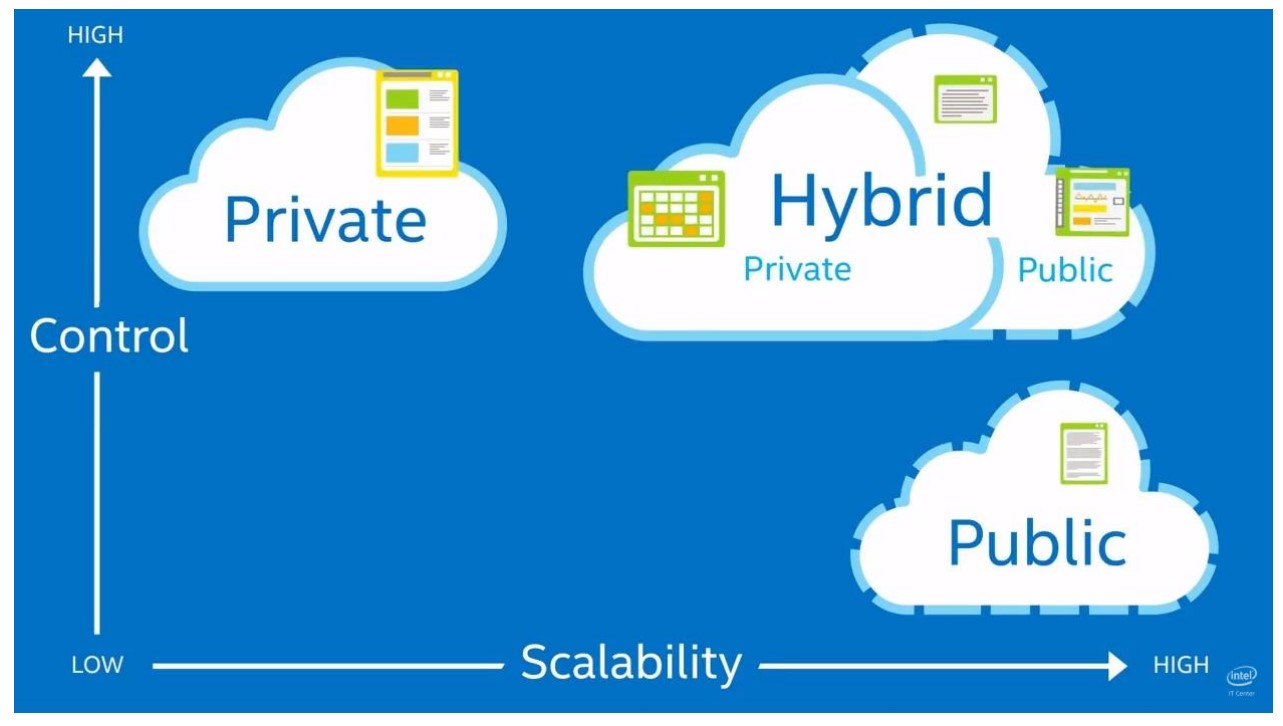
\includegraphics[width=0.7\textwidth]{immagini/Model_Deployment.jpg}
    \caption*{Model Deployment}
\end{figure}

\noindent Esistono modelli di deployment privati e pubblici, ma oggi sta avendo molto successo il Cloud ibrido:\ i dati sensibili sono mantenuti in privato, per esempio dentro l'azienda, e dove è necessaria più elasticità utilizzo un cloud pubblico.

\subsubsection{Perché si chiama Cloud?}

Perché quando si disegnava lo schema client-server tutto ciò che stava fra i due veniva rappresentato come una nuvoletta per semplicità.

\subsubsection{Ostacoli al Cloud}

\textbf{Confidenzialità dei dati}:\ Dove verranno memorizzati i nostri dati, concretamente?\ Privacy e integrità dei dati saranno garantiti?\ Come?\ Come sapremo se si è verificato un problema?

\noindent\textbf{Disponibilità dei servizi}:\ Cosa succede se un cloud provider fallisce?\ Mantra dell'informatica:\ ``no single point of failure\dots''

\noindent\textbf{Vendor lock-in}:\ rimanere ``bloccati'' con un fornitore di un servizio, per esempio dover pagare una penale per il recesso del contratto.

\section{Nuovi Modelli di Business}
Sono state innovative le idee di Dropbox, Spotify, Google.\
Dropbox ha deciso di offrire memoria gratuita a tutti, Spotify musica gratuita a tutti pagando i diritti ogni volta che viene riprodotta una canzone, mentre Google un motore di ricerca gratuito finanziandosi grazie al \textbf{customized advertising}.

\section{Green Computing}

Per costruire un computer ci vogliono due tonnellate di materiale grezzo, l'ICT in generale produce più emissioni di CO\textsubscript{2} degli aerei.\
Tra i fattori che contribuiscono all'inquinamento ci sono l'obsolescenza programmata e l'\textbf{obsolescenza} \textbf{percepita}:\ il venditore cerca di spingere il cliente ad acquistare un nuovo prodotto che avrà nuove funzionalità anche se al cliente queste non servono, ma il venditore farà in modo di fargli sentire questa ``mancanza''.\
Quindi c'è un gran numero di rifiuti tecnologici.\

In Arizona ci sono più di quaranta Data Center perché l'elettricità costa pochissimo, chiaramente le temperature del luogo richiedono grossi sistemi di raffreddamento che saranno sicuramente economici ma per niente ecologici.


\chapter{Internet Management}

\section{Overview}

Per gestire una rete, il suo traffico o la sua sicurezza è necessario prima di tutto che la rete funzioni.\
È quindi necessario un \textbf{metodo di comunicazione fra componenti di rete} per sapere se va tutto bene oppure no.\

\begin{table}[H]
    \centering
    \begin{tabular}{l l l}
        1987 & Simple Gateway Monitoring Protocol (SGMP)  &                 \\
        1987 & High-level Entity Management System (HEMS) &                 \\
        1988 & Simple Network Management Protocol         & proposed        \\
        1990 & Simple Network Management Protocol         & standard 15, 16 \\
        1991 & Management Information Base II             & standard 17     \\
        1993 & SNMP Version 2 (Party/Party/Context)       & historical      \\
        1996 & SNMP Version 2 (Communities)               & draft           \\
        1998 & SNMP Version 3 (User-based)                & draft           \\
    \end{tabular}
\end{table}

\noindent Quando furono creati i primi protocolli per la \textbf{gestione di Internet} vennero prese le idee base di ICMP:\ creare un \textbf{set d'istruzioni minimo per capire se la rete stesse funzionando ed in caso negativo cosa stesse andando male}.\
La caratteristica fondamentale di SNMP è l'essere \textbf{semplice}.\
Tale semplicità ha permesso il supporto del protocollo su apparecchi di rete con un costo ragionevole:\ ``\textit{gli switch di fascia medio-bassa possono essere gestiti tutti con SNMP}''.

SNMPv1 ha una grande diffusione soprattutto nella comunicazione dei dati.\
I tentativi di standardizzazione di SNMPv2 sono falliti.\
SNMPv3 con SNMPv1 è stato accettato da un'ampia comunità di produttori di reti.\
La comunità degli utenti ha accettato molto bene SNMPv3 in termini di supporto e sviluppo.

\subsubsection{SNMP Development Goals}

\begin{itemize}
    \item Minimizzazione del numero e della complessità delle funzioni di gestione che sono implementate da un agente:\
          \begin{itemize}
              \item Riduzione dei costi di sviluppo per agenti gestionali (applicazioni semplici).
              \item Ubiquity:\ utilizza la stessa tecnologia di gestione per tutti i dispositivi (stampanti o Cray).
              \item Estendibilità dell'applicazione:\ sviluppo di nuove funzioni di gestione senza la necessità di modificare gli agenti.
          \end{itemize}
    \item Estensibilità definendo nuovi MIB.
    \item Indipendenza da architetture di computer o di rete esistenti.
    \item Robustezza grazie a un semplice servizio di trasporto senza connessione (UDP).%attacchi DoS: in un server con un massimo di 10 connessioni, posso occupare tutte le connessioni e stare in silenzion
    \item Nessuna dipendenza da altri servizi di rete.
    \item L'aggiunta della gestione a dispositivi{\slash}applicazioni nuovi{\slash}esistenti dovrebbe essere poco costosa, semplice da sviluppare e con funzionalità limitate.
\end{itemize}
Purtroppo alcuni di questi obiettivi originari sono andati persi:\ il termine ``semplice'' si riferisce al protocollo e non alle specifiche o all'implementazione di applicazioni gestionali.

\subsubsection{Trap Directed Polling}

Il manager \textbf{esercita il controllo} su vari Agent eseguendo richieste continue (\textbf{polling}):\ poiché viene usato UDP per mandare messaggi, non è possibile conoscere gli stati degli Agent in ogni momento e quindi è necessario richiederli periodicamente; usando TCP ciò non sarebbe necessario perché la connessione persistente sarebbe sufficiente per conoscere lo stato dell'agente.\

Si ipotizzi che l'intervallo di tempo che passa fra un poll ed un altro sia di cinque minuti:\ \textbf{il Manager è cieco nei confronti dell'Agent a intervalli di cinque minuti}, ovvero assume che l'agent rimanga attivo/nello stesso stato per i cinque minuti successivi alla risposta.\
Questo non è sempre vero:\ l'Agent potrebbe ``rompersi'' subito dopo aver risposto al poll.\

Per risolvere questo problema gli Agent effettuano \textbf{trap} al Manager informandolo quando avviene un \textbf{cambio di stato importante}.\
Tuttavia l'Agent è in grado di \textbf{effettuare una trap se l'evento non è catastrofico} perciò il polling periodico è comunque necessario.\
Questo periodo di tempo varia a seconda dell'affidabilità dell'Agent con cui il Manager ha a che fare:\ \textbf{un Manager scritto bene riporta un concetto di fiducia} al suo interno, ovvero tenderà ad effettuare polling più spesso verso quegli Agent che si sono dimostrati meno affidabili.

In sintesi, i managers SNMP interrogano a intervalli regolari gli agenti SNMP:\ gli agents possono segnalare casi eccezionali a un manager inviando una trap; il manager SNMP può adattare la strategia di polling alla ricezione di trap (polling diretto da trap).

\begin{figure}[H]
    \centering
    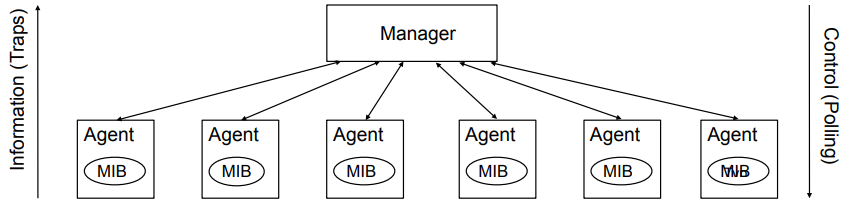
\includegraphics[width=\textwidth]{immagini/Trap_direct_polling.png}
\end{figure}

\noindent SNMP è un modello rigorosamente centralizzato, in cui il manager implementa l'intera funzionalità e responsabilità.

\subsubsection{SNMP Application Areas}

SNMP non è utilizzato solo per la gestione della rete, ma anche per il controllo e monitoraggio dei processi produttivi e dei sistemi informatici complessi e per il monitoraggio di programmi applicativi complessi (database relazionali, componenti SAP R{\slash}3,\ \dots).\

Sul mercato sono disponibili molti toolkit SNMP buoni, ma sono disponibili pochissime applicazioni per risolvere problemi di gestione complessi:\ l'implementazione di applicazioni speciali, o la conversione delle linee guida della procedura locale, in genere è relativamente complessa e costosa.

\section{Structure of Management Information \- (SMIv2)}

L'attuale modello di informazioni noto come ``\textit{Structure of Management Information version} 2'' (SMIv2) è definito e si basa su semplici variabili tipizzate, in particolar modo si basa sul sottoinsieme esteso di ASN.1 (1998).\
Ogni variabile ha un tipo di dati ASN.1 primitivo, non assemblato:
\begin{itemize}
    \item \texttt{INTEGER}, \texttt{OCTET STRING}, \texttt{OBJECT IDENTIFIER}, \texttt{NULL}
    \item \texttt{Integer32}, \texttt{Unsigned32}, \texttt{Gauge32}, \texttt{Counter32}, \texttt{Counter64}, \texttt{Ip\-Ad\-dress}, \texttt{TimeTicks}, \texttt{Opaque}
\end{itemize}
Non implementa strutture dati complesse e operazioni sulle variabili.\

Le variabili sono \textbf{scalari} (esattamente un'istanza) o colonne in una \textbf{tabella} bidimensionale ``concettuale'' (zero o più variabili) e su di esse possono essere applicate solo le operazioni di ``read'' e ``write''.\ Tuttavia il protocollo SNMP consente la manipolazione di elenchi di variabili.

I MIB (Management Information Bases) SMIv2 vengono definiti utilizzando speciali macro ASN.1.\
Sfrutta la complessità delle nuove definizioni di MIB:\ definizione di funzionalità di base e di tipi primitivi da utilizzare nei nuovi MIB.

\begin{figure}[H]
    \centering
    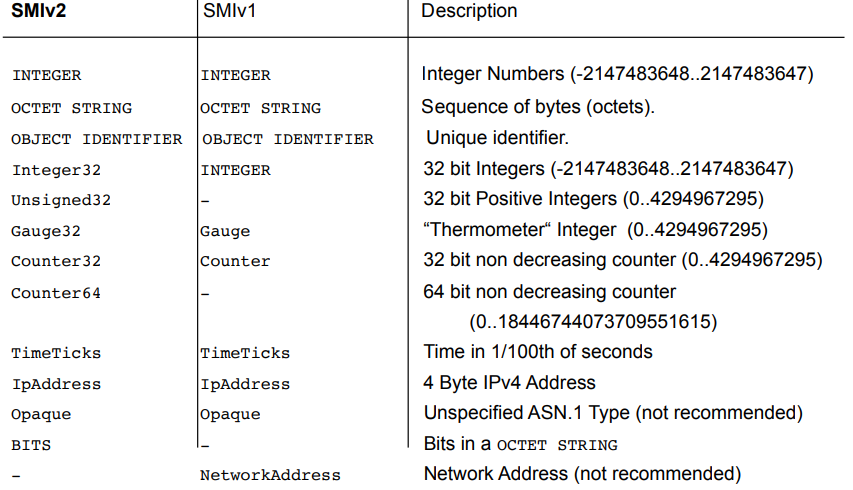
\includegraphics[width=\textwidth]{immagini/SMIv2_Basic_Datatypes.png}
    \caption*{SMIv2 Basic Datatypes (RFC 2578)}
\end{figure}

\noindent Un'altra caratteristica di SMI è che il tipo intero non si usa moltissimo, si preferisce utilizzare \texttt{gouge} e \texttt{counter}:\ sono entrambi interi ma possiedono una semantica ben precisa.\
Un \texttt{gouge} è un numero che rappresenta una quantità che va da un minimo ad un massimo.\
La temperatura, ad esempio, è un gouge (non bisogna farci calcoli sopra e può aumentare rimanendo tra un minimo ed un massimo, quando lo si legge quindi si estrapola il valore definitivo).\
Un \texttt{counter} è un intero a 32 bit come \texttt{gouge}, ma ha delle proprietà diverse:\ il contatore, infatti, non decresce (o rimane del valore corrente o aumenta) e il valore estrapolato da una variabile con questo tipo non è utilizzabile nell'immediato, ma lo si può usare per differenza (tachimetro dell'automobile e voglio sapere in un giorno quanti chilometri ho fatto).

\subsubsection{A MIB Use Case}

\begin{figure}[H]
    \centering
    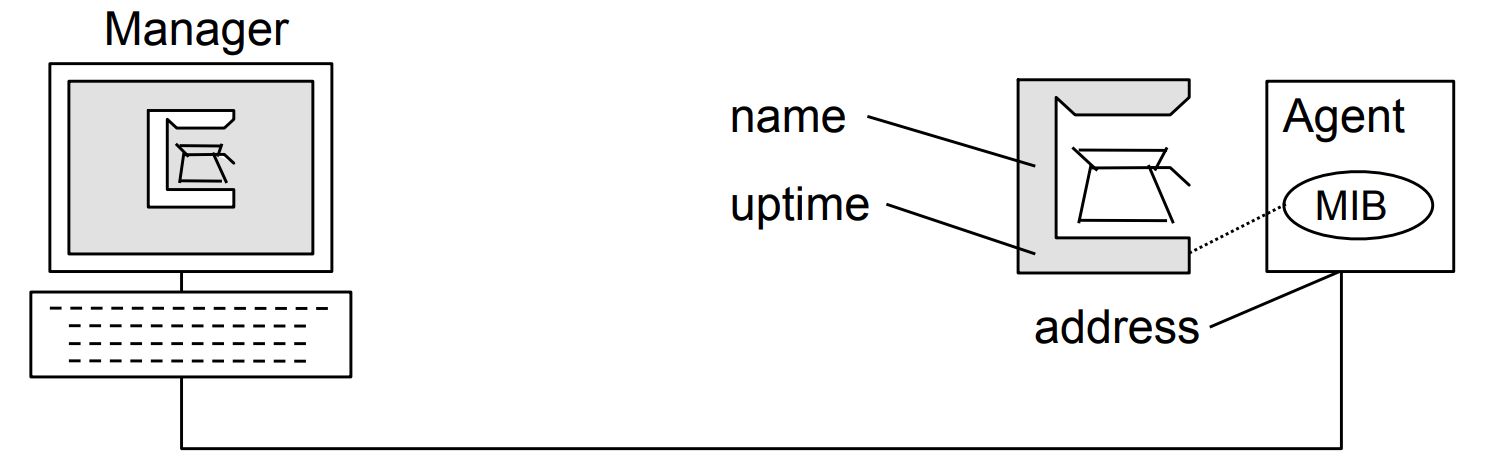
\includegraphics[width=0.8\textwidth]{immagini/MIB_useCase.png}
\end{figure}

Definizione delle variabili nell'ISO Registration tree.\
I nodi vengono definiti a scopo di denominazione.\
Le foglie dell'albero rappresentano gli oggetti gestiti (cioè ``la carne'').\
I nodi secondari possono essere utilizzati per organizzare logicamente i tipi di oggetto.\

\begin{figure}[H]
    \centering
    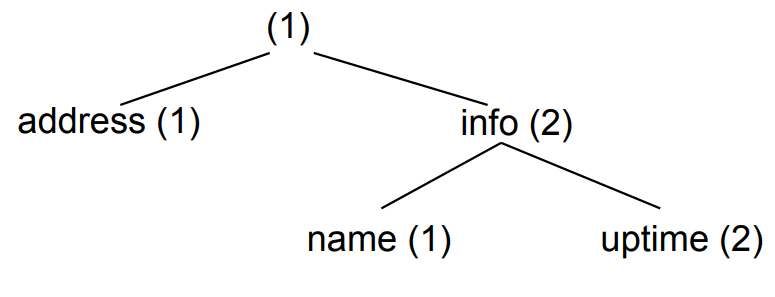
\includegraphics[width=0.5\textwidth]{immagini/ISO_registration_tree.png}
\end{figure}

\subsection{Object Identifier and Instance Identifier}

Nel Registration tree ogni oggetto può essere identificato mediante un object identifier univoco.\
Gli sviluppi concreti (istanza) di un tipo di oggetto sono designati univocamente da un cosiddetto \textit{identificatore di istanza}.\
Un identificatore di istanza univoco si ottiene allegando identificatori di istanza all'identificatore di oggetto.

Gli oggetti scalari hanno fondamentalmente \textbf{una sola istanza} il cui identificatore ha valore 0 (e.g.\ \texttt{sysName.0}).\
Gli identificatori di istanza per le variabili non scalari derivano dalla denominazione univoca di una tabella concettuale.\
Poiché l'identificatore di oggetto può contenere fino a 128 elementi, i nomi delle istanze non possono essere infinitamente complessi.
\begin{figure}[H]
    \centering
    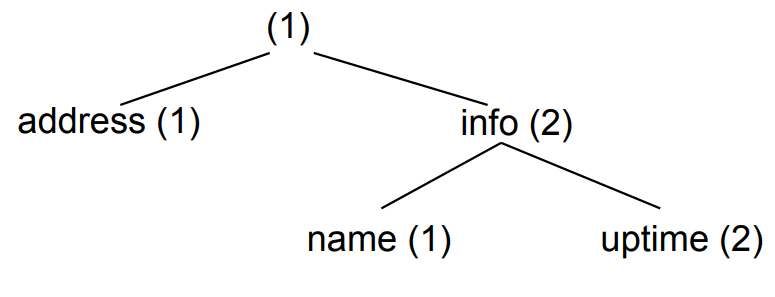
\includegraphics[width=0.5\textwidth]{immagini/ISO_registration_tree.png}
\end{figure}
\begin{table}[H]
    \centering
    \begin{tabular}{|l l l l|}
        \hline
        Object Identifier & Instance Identifier & Type                  & Value           \\\hline
        1.1               & 0                   & \texttt{IpAddress}    & 10.1.2.1        \\
        1.2.1             & 0                   & \texttt{OCTET STRING} & ``FilterFresh'' \\
        1.2.2             & 0                   & \texttt{TimeTicks}    & 54321           \\\hline
    \end{tabular}
\end{table}

\noindent I nomi dei nodi MIB sono rilevanti solo per gli utenti umani.

I descrittori devono essere univoci all'interno di un modulo MIB, sebbene possano essere utilizzati più volte in diversi moduli MIB (si ottengono descrittori univoci dalla combinazione dei nomi dei moduli e dei descrittori).

\begin{figure}[H]
    \centering
    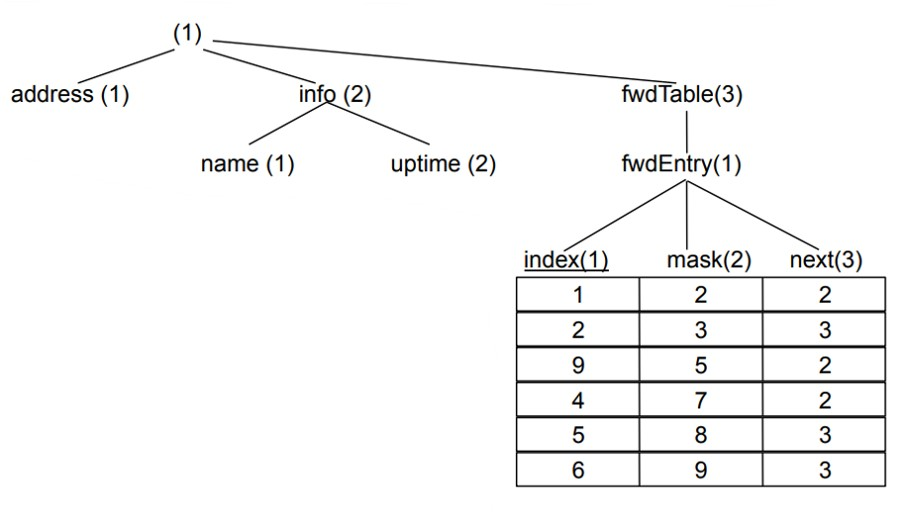
\includegraphics[width=0.7\textwidth]{immagini/Tables_MIB.jpg}
\end{figure}

\noindent Le tabelle sono definite fondamentalmente con due ``nodi ausiliari'':\ il primo nodo definisce la tabella ed è di tipo \texttt{SEQUENCE OF}, mentre il secondo nodo definisce una voce (una riga) nella tabella ed è di tipo \texttt{SEQUENCE}; questo è l'unico uso consentito di \texttt{SEQUENCE} e \texttt{SEQUENCE OF} in SNMP SMIv2.\

Il risultato della colonna e dell'identificatore di istanza (codice della tabella) è un identificatore di oggetto univoco per ciascuna voce di tabella.

\begin{table}[H]
    \centering
    \begin{tabular}{|l l l|l l l|l l l|}
        \multicolumn{9}{c}{Esempio di tabella (convenzione OID $\Rightarrow$ valore):}                          \\\hline
        1.3.1.1.1 & $\Rightarrow$ & 1 & 1.3.1.3.1 & $\Rightarrow$ & 2 & 1.3.1.2.4 & $\Rightarrow$ & 7           \\
        1.3.1.2.1 & $\Rightarrow$ & 2 & 1.3.1.1.4 & $\Rightarrow$ & 4 & 1.3.1.2.7 & $\Rightarrow$ & inesistente \\\hline
    \end{tabular}
\end{table}

\subsubsection{Tables Naming}

La denominazione delle tabelle è molto importante poiché influisce sul modo in cui si accede alle tabelle stesse.\
Ne esistono due tipi:\ uno usa numeri di riga (non utilizzati da SNMP), l'altro usa una colonna indice (il metodo usato da SNMP).

Un indice di tabella non è necessariamente un \texttt{INTEGER}, ad esempio la routing table utilizza un indirizzo IP come indice della tabella.

\begin{table}[H]
    \centering
    \begin{tabular}{|l|c|l|}
        \hline
        \multicolumn{3}{|c|}{Routing Table}                                   \\\hline\hline
        \texttt{destination}(1) & \texttt{policy}(2) & \texttt{next}(3)       \\\hline
        \texttt{130.89.16.23}   & 1                  & \texttt{130.89.16.23}  \\
        \texttt{130.89.16.23}   & 2                  & \texttt{130.89.16.127} \\
        \texttt{192.168.10.12}  & 1                  & \texttt{172.16.1.18}   \\
        \texttt{192.168.10.12}  & 2                  & \texttt{172.16.1.12}   \\\hline
    \end{tabular}
\end{table}

\noindent Un indice di tabella può essere composto da più componenti:

\begin{center}
    X .\ C .\ I\textsubscript{1} .\ I\textsubscript{2} \dots\dots\ I\textsubscript{n}
\end{center}

\begin{table}[H]
    \centering
    \begin{tabular}{c l}
        X                   & OID of the table:\ identifica la tabella \\
        C                   & Column number:\ identifica la colonna    \\
        $\rm I_1 \dots I_n$ & Index value (indice nella colonna)       \\
    \end{tabular}
\end{table}

\noindent Una tabella di routing IP è la combinazione di indirizzo IP e maschera di rete IP necessaria per soddisfare le regole di instradamento.\
I singoli byte dell'indirizzo IP vengono specificati come identificatori secondari individuali.

\begin{figure}[H]
    \centering
    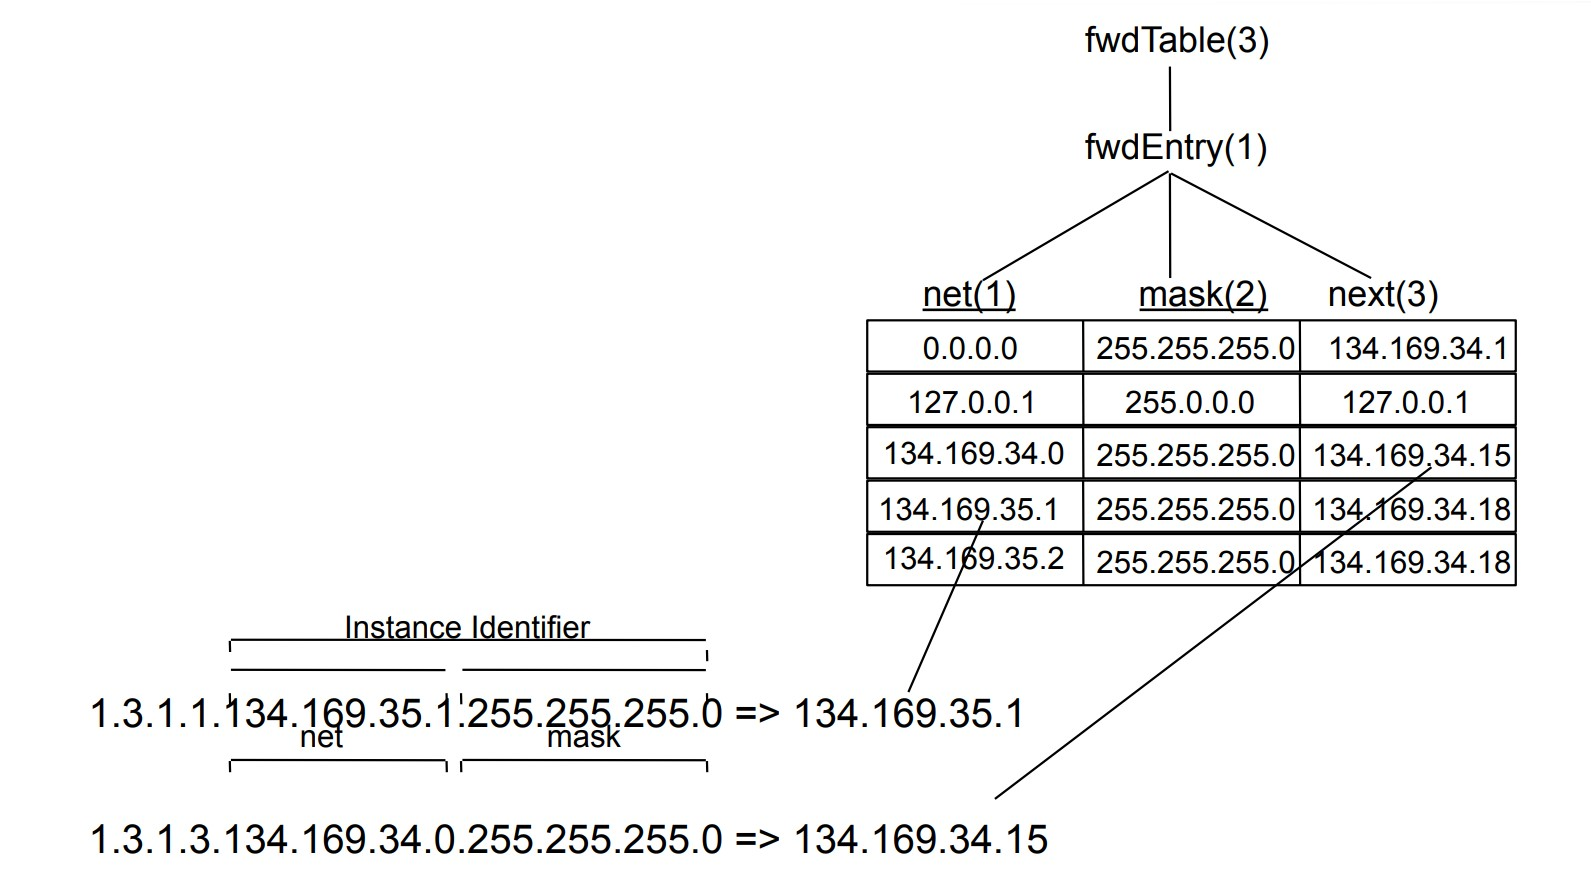
\includegraphics[width=0.9\textwidth]{immagini/RoutingTable.jpg}
\end{figure}

\subsubsection{Rules for the Specification of Instance Identifier values}

Valori per tipi fondamentali:

\begin{itemize}
    \item Valori per \texttt{INTEGER}:\ un singolo valore intero.
    \item Valori per \texttt{OCTET STRING} di lunghezza fissa:\ ogni singolo byte viene trattato come un valore individuale.
    \item Valori per \texttt{OCTET STRING} di lunghezza variabile:\ il primo valore è la lunghezza, seguita da ogni singolo byte.
    \item Valori per \texttt{OBJECT IDENTIFIER}:\ il primo valore è la lunghezza, seguita da ogni singolo byte.
\end{itemize}
La parola chiave \texttt{IMPLIED} può essere utilizzata senza il byte di lunghezza se non porta ad ambiguità.

La lunghezza massima dei valori \texttt{OBJECT IDENTIFIER} è limitata a 128 elementi, quindi gli identificatori di istanza non saranno complessi arbitrari.

\subsection{MIB Module}

Tipi di oggetti simili vengono combinati in moduli MIB,  ogni modulo MIB deve avere un nome univoco (lettere maiuscole).\
I moduli MIB sono (quasi) normali moduli ASN.1 e obbediscono alle regole lessicali ASN.1.\
Le definizioni possono essere importate da altri moduli MIB con l'aiuto dell'istruzione \texttt{IMPORT}; tutte le macro ASN.1 SMI utilizzate devono essere importate esplicitamente.

\begin{verbatim}
COFFEE-MIB DEFINITIONS ::= BEGIN

IMPORT      MODULE-IDENTITY, OBJECT-TYPE, enterprises,
            IpAddress, TimeTicks    FROM SNMPv2-SMI;
...
END
\end{verbatim}

\subsubsection{Module-Identities (RFC 2578)}

\begin{verbatim}
<descriptor> MODULE-IDENTITY
        LAST-UPDATED <ExtUTCTime>
        ORGANIZATION <Text>
        CONTACT-INFO <Text>
        DESCRIPTION <Text>
        [REVISION <ExtUTCTime>
        DESCRIPTION <Text>]*
        ::= <ObjectIdentifier>
\end{verbatim}
Definisce le informazioni amministrative, ad es.\ informazioni di contatto e numero di versione.\
Le clausole \texttt{REVISION} e \texttt{DESCRIPTION} non sono obbligatorie e possono ripetersi più volte.

\begin{figure}[H]
    \centering
    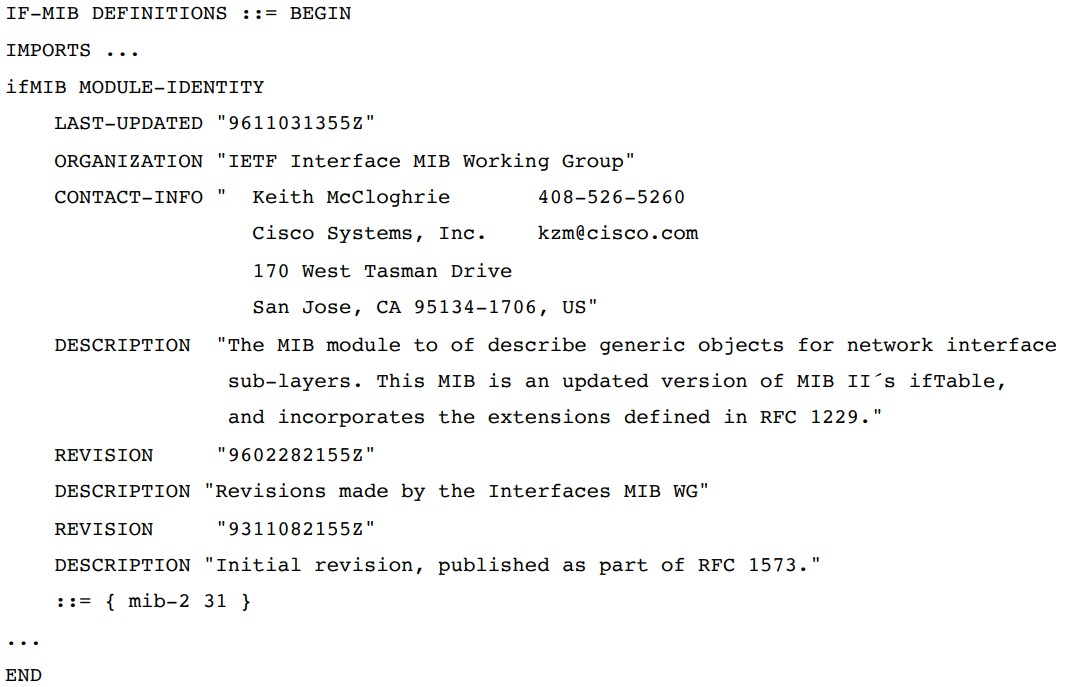
\includegraphics[width=\textwidth]{immagini/Module_Identities.jpg}
    \caption*{Esempio di Module Identities}
\end{figure}

\subsubsection{Object Identities (RFC 2578)}

\begin{verbatim}
<descriptor> OBJECT-IDENTITY
        STATUS <Status>
        DESCRIPTION <Text>
        [REFERENCE <Text>]
        ::= <ObjectIdentifier>

\end{verbatim}
Definisce e registra un valore dell'identificatore di oggetto:\ consente l'allocazione di qualsiasi nodo all'interno dell'albero di registrazione.\

La clausola \texttt{STATUS} definisce se il nodo allocato è ``obsoleto'', ``corrente'' o ``deprecato''.\
Il \texttt{REFERENCE} opzionale viene utilizzato per fare riferimento a ulteriori informazioni (simile ai collegamenti ipertestuali HTML).

\begin{figure}[H]
    \centering
    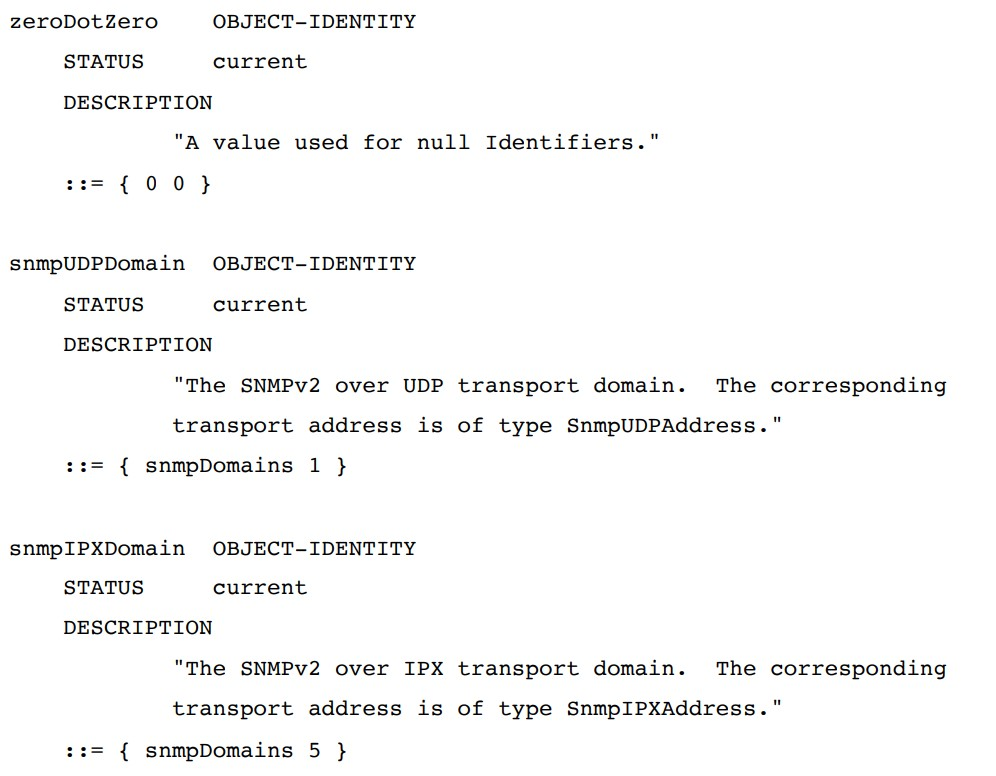
\includegraphics[width=\textwidth]{immagini/ObjectIdentities.jpg}
    \caption*{Esempio di Object Identities}
    \label{fig:my_label}
\end{figure}

\subsubsection{Object Types (RFC 2578)}

\begin{verbatim}
<descriptor> OBJECT-TYPE
        SYNTAX <Syntax>
        [UNITS <Text>]
        MAX-ACCESS <Access>
        STATUS <Status>
        DESCRIPTION <Text>
        [REFERENCE <Text>]
        [INDEX <Index>]
        [AUGMENTS <Index>]
        [DEFVAL <Value>]
        ::= <ObjectIdentifier>
\end{verbatim}
Macro per la definizione di tipologie di oggetti e tabelle concettuali.

Le clausole \texttt{INDEX} e \texttt{AUGMENTS} sono consentite solo per la definizione mediante tabelle.\
Esattamente una delle clausole precedenti deve essere specificata durante la definizione della tabella.

\begin{figure}[H]
    \centering
    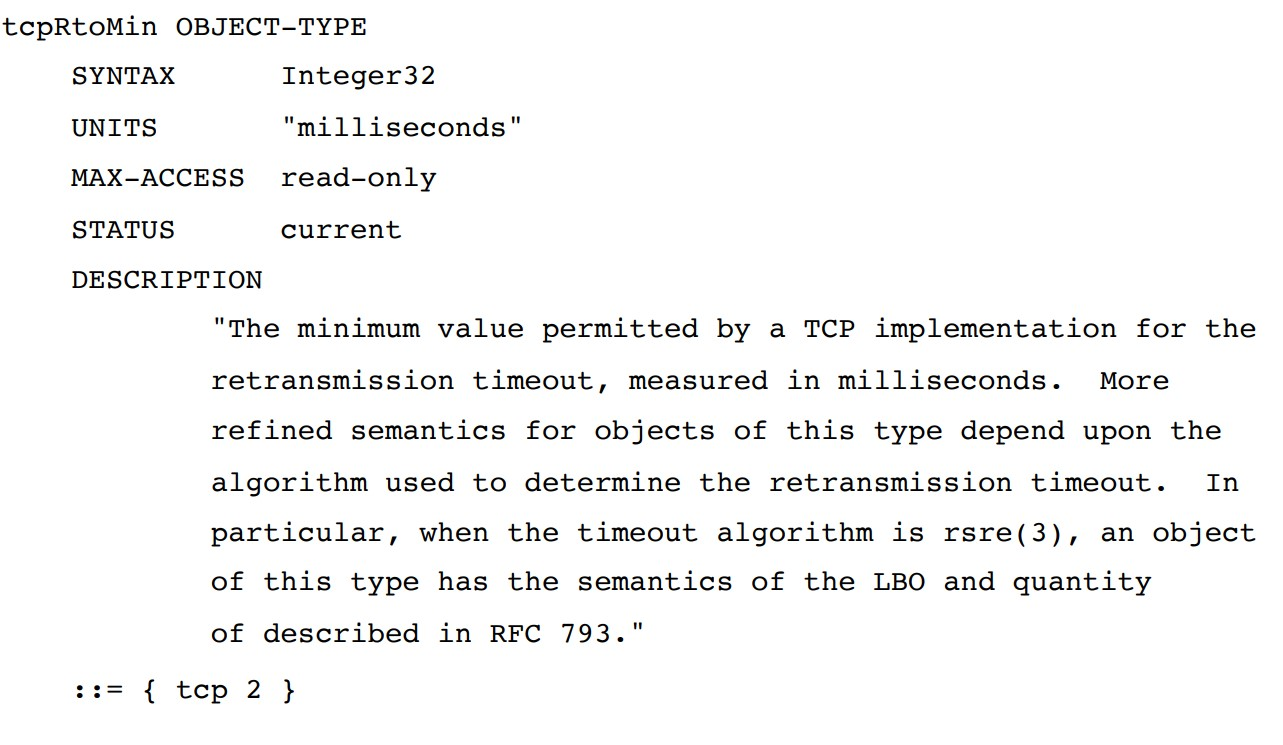
\includegraphics[width=\textwidth]{immagini/Object_Types.jpg}
    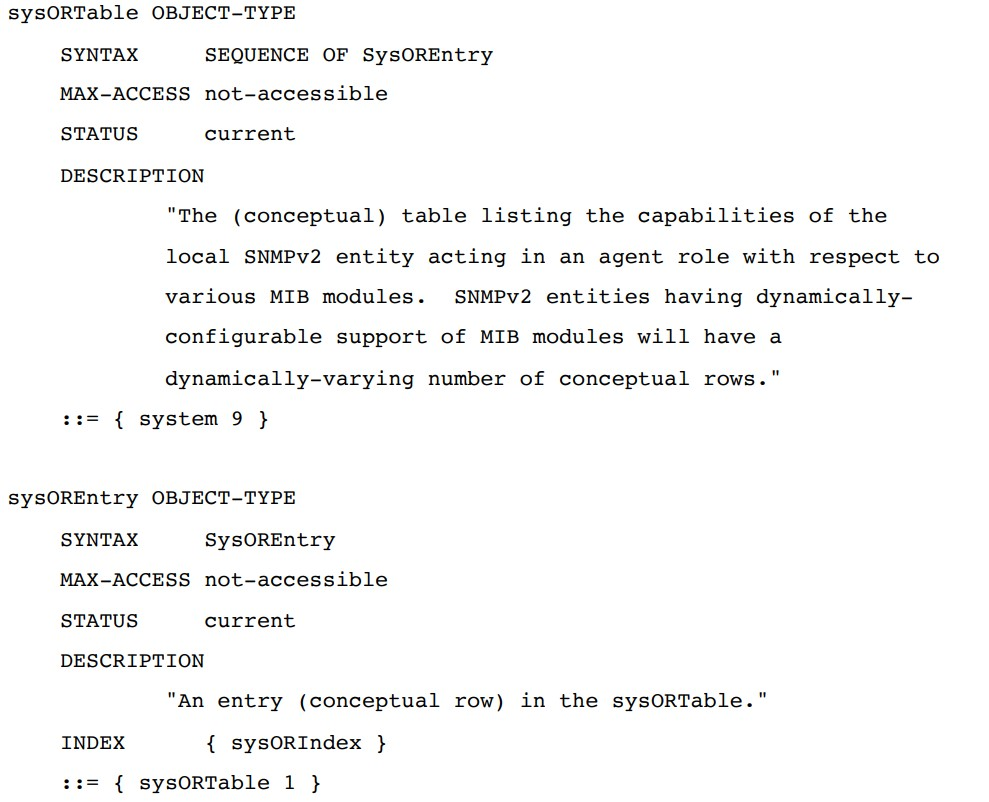
\includegraphics[width=\textwidth]{immagini/Object_Types2.jpg}
\end{figure}

\subsubsection{Notification-Types (RFC 2578)}

\begin{verbatim}
<descriptor> NOTIFICATION-TYPE
        [OBJECTS <Objects>]
        STATUS <Status>
        DESCRIPTION <Text>
        [REFERENCE <Text>]
        ::= <ObjectIdentifier>
\end{verbatim}

\noindent Macro per la registrazione di un evento; in caso di evento, un manager o un agente può inviare una notifica appropriata a un altro manager.

Le clausole \texttt{OBJECTS} definiscono quali oggetti MIB devono essere contenuti nella descrizione dell'evento.\
La clausola \texttt{DESCRIPTION} deve descrivere quali istanze si intendono caso per caso.

\subsubsection{New Types from Textual Conventions}

In SNMP non si possono definire nuovi tipi di dato, per questa ragione si utilizza la \textbf{textual convention} ridefinendo tipi di dato già esistenti per definire un tipo di dato dal punto di vista della rappresentazione.\
Tuttavia, altri tipi potrebbero non essere derivati da una \textit{textual convention}.\
Una clausola \texttt{DISPLAY-HINT} definisce una semplice figura della rappresentazione ASN.1 di un valore in un formato leggibile per gli esseri umani.\
La clausola \texttt{DISPLAY-HINT} può essere utilizzata solo insieme al tipo di dati \texttt{INTEGER} e \texttt{OCTET STRING} e da cui deriva.\

Si noti che una \textit{textual convention} può determinare restrizioni sull'ambito e non può definire un tipo assemblato.

Le convenzioni testuali sono definite nella RFC 2579.
\begin{verbatim}
<descriptor> ::= TEXTUAL-CONVENTION
        [DISPLAY-HINT <Text>]
        STATUS <Status>
        DESCRIPTION <Text>
        [REFERENCE <Text>]
        SYNTAX <Syntax>
\end{verbatim}

\noindent La clausola \texttt{DISPLAY-HINT} definisce una figura bidirezionale della rappresentazione utilizzata internamente su una rappresentazione leggibile per gli esseri umani.\
Nella clausola \texttt{SYNTAX} possono essere utilizzati solo tipi di dati di base (si possono quindi limitare ulteriormente le convenzioni testuali non esistenti).

Tutte le altre semantiche devono essere definite nella clausola \texttt{DESCRIP\-TION}.

\subsubsection{Further SMIv2 Macros}

SMI definisce delle macro su ASN.1 che permettono di raggruppare gli oggetti tra di loro.\
Quando si creano dei MIB, è possibile che i vari oggetti implementino solo una parte dell'intera funzionalità.\
Queste macro hanno la possibilità di dividere gli oggetti in gruppi, così facendo sarà presente un \textbf{gruppo minimo}, ovvero il modulo del dispositivo che permetterà a quest'ultimo di essere conforme alla specifica.

\begin{itemize}
    \item \texttt{OBJECT-GROUPS}:\ consente la definizione di gruppi di tipi di oggetti correlati; questa macro può essere utilizzata nella macro \texttt{MODULE-COMPLI\-ANCE}.
    \item \texttt{NOTIFICATION-GROUPS}:\ consente la definizione di gruppi di tipi di notifica correlati; questa macro può essere utilizzata nella macro \texttt{MOD\-ULE-COMPLIANCE}.
    \item \texttt{MODULE-COMPLIANCE}:\ definisce uno o più vincoli che le implementazioni MIB devono soddisfare.
    \item \texttt{AGENT-CAPABILITIES}:\ descrive le capacità di un'implementazione MIB reale.
\end{itemize}

\subsection{MIB-Compiler}

\begin{figure}[H]
    \centering
    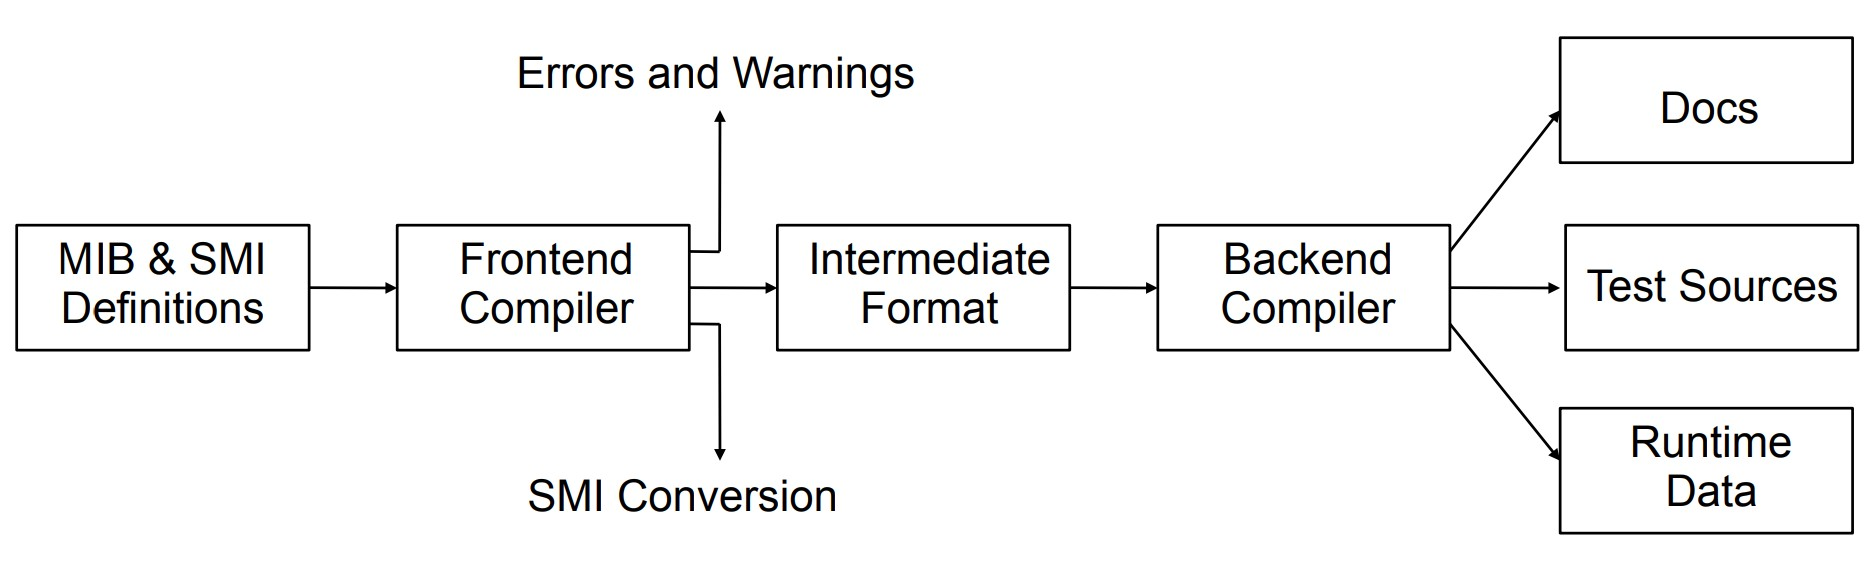
\includegraphics[width=\textwidth]{immagini/MIB_Compiler.jpg}
\end{figure}

Gli oggetti una volta definiti vengono scritti in formato testuale sul file system e possono essere utilizzati per più fini.\
Prima di eseguire una conversione di formato avviene una \textit{verifica formale} allo scopo di verificare l'assenza di problemi; questa operazione risulta particolarmente utile nelle fasi di \texttt{IMPORT} da un altro oggetto.\
Se la verifica formale va a buon fine si ottiene una rappresentazione intermedia per il backend-compiler, il quale può produrre la documentazione (utilizzando le descrizioni presenti nei notification typer, object identities, \dots), dei test case per verificare se l'implementazione è corretta (se ho una variabile definita come read-only, il test deve fallire in caso si provi a fare una scrittura) e i run time data (generati dopo la lettura dei dati).

\textbf{Osservazione}:\ non esiste un formato intermedio standardizzato o generalmente accettato.

\section{Fundamental MIBs}

MIB-II (RFC 1213) definisce i tipi di oggetto per i protocolli Internet IP, ICMP, UDP, TCP, SNMP (e altre definizioni non rilevanti qui); fondamentalmente modella la gestione dello stack del protocollo TCP/IP.\
La definizione MIB-II ha come obiettivi definire gli errori di base e la gestione della configurazione per i protocolli Internet, evitare informazioni ridondanti nel MIB e avere pochissimi e deboli oggetti di controllo.\
Inoltre, l'implementazione del MIB non dovrebbe interferire con le normali attività di rete e nessun tipo di oggetto deve dipendere da essa.

Complessivamente 170 tipi di oggetti:\ alcune definizioni MIB si sono rivelate troppo semplici e minime (tabella di instradamento, tabella di interfaccia), mentre altre presuppongono un formato di indirizzo a 4 byte, quindi queste tabelle devono essere ridefinite per IP versione 6 (IPv6).

\begin{figure}[H]
    \centering
    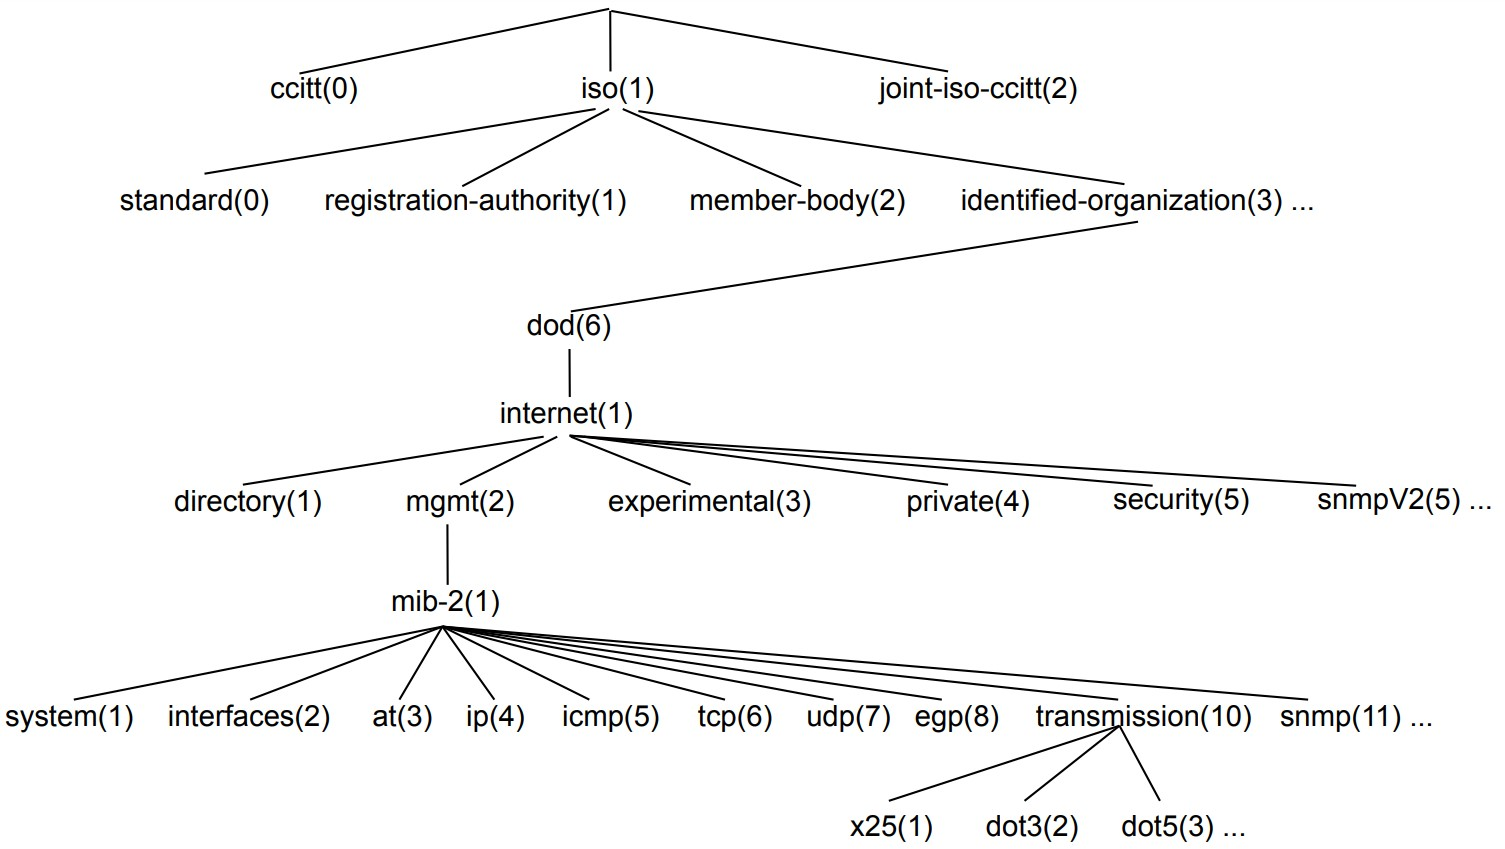
\includegraphics[width=\textwidth]{immagini/StructureMIBII.jpg}
\end{figure}

\noindent Il MIB-II è uno dei più importanti perché è nato con SNMP ed ha portato alla diffusione di quest'ultimo:\ il protocollo http è utile fin tanto che ci sono siti web da leggere, MIB-II funge da sito web, infatti all'interno di quest'ultimo sono presenti le informazioni di monitoraggio da analizzare con SNMP.\
Infine, MIB-II è importante perché permette di gestire tutte quelle che sono le informazioni di base di un sistema basato su SNMP (informazioni sulle interfacce di rete, sull'ARP table, sul protocollo IP, sull'ICMP, \dots).

\subsubsection{Osservazioni su MIB-II}

\begin{itemize}
    \item Il ramo ``\texttt{transmission}'' ospita tutte le definizioni MIB che si occupano della trasmissione delle informazioni (X.25, PPP, RS232, SONET, ISDN, IEEE 802.3, IEEE 802.5, FDDI,\ \dots)
    \item Il ramo ``\texttt{at}'' (ARP Table) è stato sostituito da un'estensione del gruppo di IP.
    \item Il ramo \texttt{egp} (External Gateway Protocol) non è più utilizzato in quanto il protocollo EGP al giorno d'oggi non ha alcuna importanza.
    \item Molti altri moduli MIB sono stati registrati nel nodo ``\texttt{mib-2}''.\ L'assegnazione dei numeri di registrazione è delegata allo IANA (Internet Assigned Numbers Authority).
    \item In questi giorni sarebbe bene introdurre una certa modularità nel MIB in modo che i diversi rami possano essere aggiornati in modo indipendente.\
\end{itemize}

\section{SNMP Version 1}

\begin{figure}[H]
    \centering
    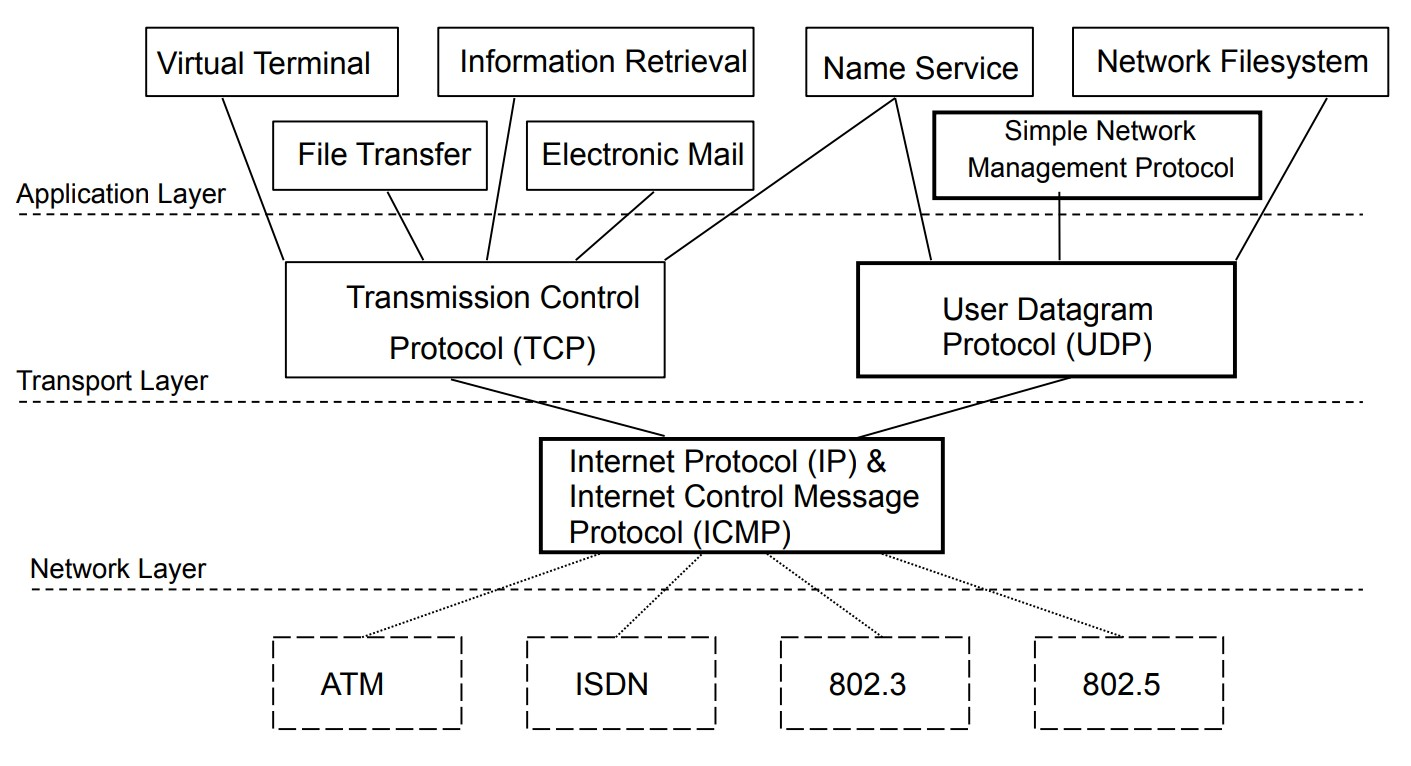
\includegraphics[width=0.9\textwidth]{immagini/SNMP.jpg}
\end{figure}

\textbf{SNMP} (\textit{Simple Network Management Protocol}) si trova nella parte alta dello stack TCP{\slash}IP, nell'Application Layer.\
Nel caso del mondo ISO{\slash}OSI corrisponde al livello 7, dove si trovano le applicazioni usate dagli utenti.\

È un protocollo che sfrutta \textbf{UDP} come servizio del livello di transporto, perciò si tratta di un protocollo \textit{connectionless}.\
In realtà esiste anche una versione che supporta il protocollo TCP, tuttavia si privilegia quella che fa uso di UDP.\

\subsubsection{Ordinamento lessicografico}

Le istanze MIB sono disposte nel MIB lessicograficamente in base al valore dell'identificatore di oggetto che identifica l'istanza.\
Il registro SNMP utilizza questa caratteristica per leggere (\textit{walk}) tabelle concettuali o MIB sconosciuti.\

\begin{table}[H]
    \centering
    \begin{tabular}{|l|l|l|l|}
        \hline
        \textbf{Object Identifier} & \textbf{Value}  & \textbf{Object Identifier} & \textbf{Value} \\\hline \hline
        1.1.0                      & 10.1.2.3        & 1.3.1.2.3                  & 5              \\
        1.2.1.0                    & ``FilterFresh'' & 1.3.1.2.4                  & 7              \\
        1.2.2.0                    & 54321           & 1.3.1.2.5                  & 8              \\
        1.3.1.1.1                  & 1               & 1.3.1.2.6                  & 9              \\
        1.3.1.1.2                  & 2               & 1.3.1.3.1                  & 2              \\
        1.3.1.1.3                  & 3               & 1.3.1.3.2                  & 3              \\
        1.3.1.1.4                  & 4               & 1.3.1.3.3                  & 2              \\
        1.3.1.1.5                  & 5               & 1.3.1.3.4                  & 2              \\
        1.3.1.1.6                  & 6               & 1.3.1.3.5                  & 3              \\
        1.3.1.2.1                  & 2               & 1.3.1.3.6                  & 3              \\
        1.3.1.2.2                  & 3               &                            &                \\\hline
    \end{tabular}
    \caption*{Esempio di ordinamento lessicografico}
\end{table}

\noindent Con questo ordinamento la struttura concettuale della tabella viene persa poiché l'output del percorso è un elenco e non più una tabella.\

Il protocollo SNMP opera solo su questo elenco organizzato.

\subsubsection{SNMPv1 operations}

Le primitive principali di SNMPv1 sono
\begin{table}[H]
    \centering
    \begin{tabular}{l l}
        \texttt{get}     & legge il valore di un Object Identifier                            \\
        \texttt{getNext} & legge il valore dell'Object Identifier successivo a quello attuale \\
        \texttt{set}     & imposta il valore relativo a un Object Identifier                  \\
        \texttt{trap}    & manda una notifica al manager                                      \\
    \end{tabular}
\end{table}

\noindent Le prime tre operazioni sono sempre ``iniziate'' dal manager, la \texttt{trap} è l'unica che permette all'agent di contattare il manager:\ è necessaria per mandare una notifica relativa a un cambio di stato al manager poiché usare il \textit{polling} sarebbe poco efficiente (poco scalabile) e poco sicuro.\
Se si utilizzassero solo le trap senza il ciclo di polling, nessuno controllerebbe che gli agent abbiano svolto correttamente il loro lavoro e il loro funzionamento (operazione che in origine era affibbiata al manager mediante il polling).\
In SNMP c'è il problema di \textbf{agent unreachable}:\ il manager pensa che stia andando tutto bene, mentre l'agent sta cercando di mandargli messaggi informativi che però non arrivano a causa di un guasto alla rete.\

L'approccio SNMP è sensato se il numero di dispositivi (agent) da controllare è piccolo; se la quantità di dispositivi da monitorare è molto grande, c'è la necessità di arricchire le trap da parte degli agent rendendole più potenti:\ per esempio, nel caso di uno switch a 48 porte, la trap deve coprire lo spazio di gestione di tutte le porte.\

\begin{figure}[H]
    \centering
    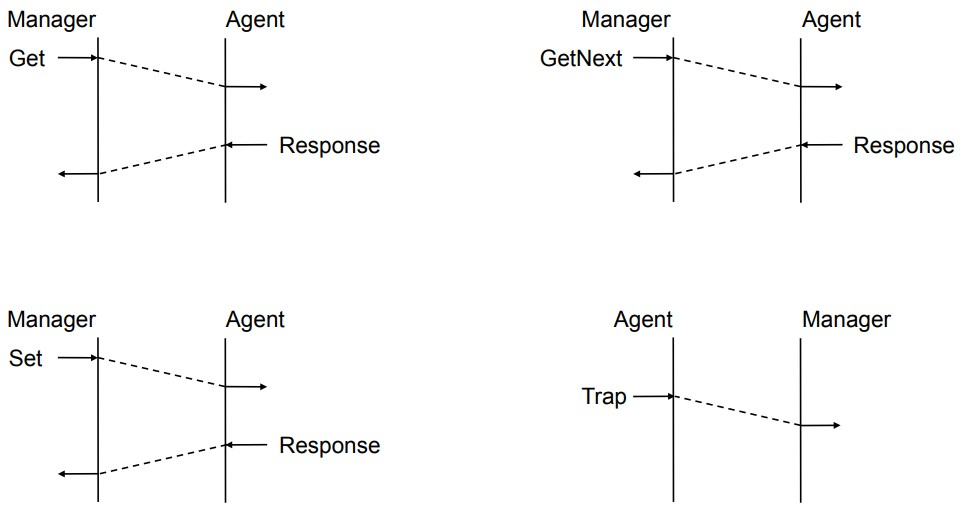
\includegraphics[width=0.9\textwidth]{immagini/SNMP_operations.jpg}
\end{figure}

\noindent\textbf{Nota}:\ il protocollo SNMP può scambiare solo (un elenco di) scalari.

\subsection{Formato messaggi SNMPv1}

Il primo campo dei messaggi SNMP contiene la \textit{versione}.\
Il secondo campo contiene una stringa, \textit{community}, usata per l'autenticazione degli utenti (controllo sui diritti, come una password).

\begin{figure}[H]
    \centering
    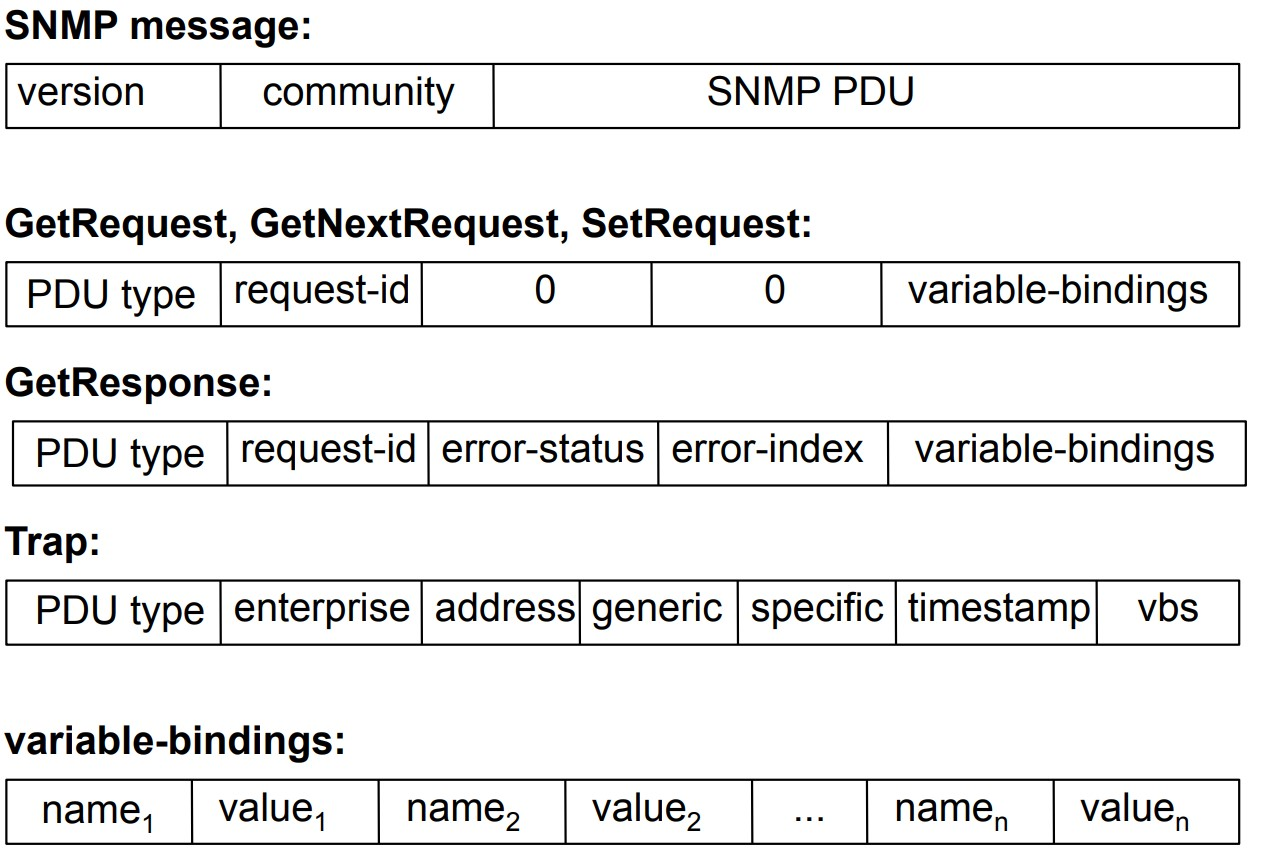
\includegraphics[width=0.8\textwidth]{immagini/SNMP_messageFormat.jpg}
\end{figure}

\noindent Infine vi è il \textbf{PDU} (\textit{Protocol Data Unit}) che varia a seconda del tipo di messaggio.\ Nel caso della request la \texttt{get}, la \texttt{getNext} e la \texttt{set} contengono un'identificativo unico della richiesta usato per ``legare'' la successiva risposta e un campo contenente una serie di \verb|<Object Identifier, valore>|:\ $\simeq$ 1400 byte a disposizione, nel caso in cui si sfori tale dimensione l'invio del messaggio fallisce e viene generato un codice di errore specifico.\ La \texttt{trap} ha un formato diverso.\

All'inizio di ogni PDU vi è un campo \texttt{type} per distinguere il tipo di messaggio.\

\textbf{Osservazione}:\ l'agent gestisce le richieste in modo atomico (una richiesta per volta), quelle che vengono ricevute e che non possono essere elaborate vengono accodate.\
Se le primitive vengono eseguite su un singolo object-ID piuttosto che su un insieme si perde la proprietà di atomicità (le richieste in questo caso vengono gestite come nei programmi multithreaded).

\subsubsection{Get Operation}

L'operazione \texttt{get} può essere utilizzata per leggere una o più variabili.\
Possibili errori durante l'elaborazione di un'operazione \texttt{get}:
\begin{table}[H]
    \centering
    \begin{tabular}{l l}
        \texttt{noSuchName} & l'istanza richiesta non esiste o non è una foglia             \\
        \texttt{tooBig}     & il risultato della richiesta non rientra nella risposta (UDP) \\
        \texttt{genErr}     & si è verificato qualsiasi altro errore                        \\
    \end{tabular}
\end{table}

\noindent In caso di più errori, solo un errore viene segnalato come indice di errore e stato di errore sono univoci nella PDU.

\subsubsection{GetNext Operation}

Recupera il nome dell'oggetto e il valore dell'istanza successiva, viene utilizzata per rilevare le strutture MIB e leggere le tabelle.\

\texttt{getNext} consente di leggere le istanze MIB secondo l'ordine lessicografico:\ utilizzando più{\slash}successive operazioni \texttt{getNext} è possibile leggere l'intero MIB senza conoscerne la struttura.\
Possibili errori durante l'elaborazione di un'operazione \texttt{getNext}:

\begin{table}[H]
    \begin{tabular}{l l}
        \texttt{noSuchName} & l'istanza richiesta non esiste (= fine del MIB)               \\
        \texttt{tooBig}     & il risultato della richiesta non rientra nella risposta (UDP) \\
        \texttt{genErr}     & si è verificato qualsiasi altro errore                        \\
    \end{tabular}
\end{table}

\subsubsection{Set Operation}

L'operazione di \texttt{set} scrive i valori in una o più istanze MIB atomicamente.\
Con l'aiuto dell'operazione \texttt{set} è possibile creare anche nuove istanze MIB, se la definizione MIB lo consente (non esiste una procedura standard definita in SNMPv1 per la creazione dell'istanza).\
Possibili errori durante l'elaborazione di un'operazione \texttt{set}:

\begin{table}[H]
    \begin{tabular}{l l}
        \texttt{noSuchName} & l'istanza richiesta non esiste e non può essere creata        \\
        \texttt{badValue}   & il valore specificato è di tipo sbagliato                     \\
        \texttt{tooBig}     & il risultato della richiesta non rientra nella risposta (UDP) \\
        \texttt{genErr}     & si è verificato qualsiasi altro errore                        \\
    \end{tabular}
\end{table}

\noindent Viene definito anche il codice di errore \texttt{readOnly}, ma generalmente non viene usato.

\subsubsection{Trap Operation}

Con l'operazione \texttt{trap} gli agents possono informare un manager riguardo un evento; poiché non si vogliono mischiare i traffici di \texttt{get} e \texttt{set} con quelli di \texttt{trap}, in questo caso si usa la porta 162.\

Per ricevere queste trap, il Manager deve avere un demone sulla porta 162 che resta in ascolto e le gestisce.\
Nel caso più comune, se non vi è nessuno ad ascoltare il traffico in arrivo o la macchina è spenta, i pacchetti vengono persi.\ Nel caso meno comune vengono comunque persi ma viene anche inviato un messaggio ICMP \texttt{destination unreachable} alla sorgente dei messaggi.\
\textbf{Nota}:\ un manager può essere configurato per ignorare le traps!\

La ricezione di un'operazione \texttt{trap} non è riscontrata, quindi non è affidabile in quanto può essere persa durante il trasferimento.\
La generazione di traps può portare alle cosiddette ``\textit{trap storm}'', ad esempio se dopo un'interruzione di corrente tutti i dispositivi vogliono visualizzare contemporaneamente il riavvio.\
Gli agenti possono essere normalmente configurati con gli indirizzi IP degli host in cui è possibile inviare trap, tuttavia non esiste una tecnica standard in SNMPv1 per tale configurazione dell'agente:\ di solito viene utilizzato un file di configurazione (non il MIB).\
Sebbene si utilizzino le traps, il polling è ancora necessario (ad esempio, l'agente potrebbe essere inattivo).\

\section{SNMP Version 2c}

Il termine SNMPv2 è ambiguo.\
SNMPv2c doveva risolvere i problemi della v1 tra cui l'autenticazione; la sola presenza della \textit{comunità} come misura di sicurezza (che passava in chiaro) non era abbastanza considerando che al tempo venivano usati gli hub:\ il traffico veniva mandato ovunque nelle reti locali ed era quindi molto semplice reperire la ``password'' da usare per eseguire primitve SNMP.\
Esistono alcune varianti di SNMP versione 2:
\begin{itemize}
    \item SNMPv2p:\ Versione con modello di sicurezza basato sulle parti, storico.
    \item SNMPv2c:\ SNMPv2 con banale modello di sicurezza basato sulla comunità, sperimentale.
    \item SNMPv2u:\ SNMPv2 con un modello di sicurezza basato sull'utente, storico.
    \item SNMPv2*:\ SNMPv2 con modello di sicurezza e amministrazione, storico.
\end{itemize}
Ci furono varie proposte ma il loro sviluppo andava per le lunghe quindi la community venne lasciata e SNMPv2 diventò SNMPv2c.\
Quest'ultimo ha riscontrato una certa diffusione, sebbene IETF non lo abbia mai standardizzato.\

Sono state aggiunte le \textbf{eccezioni}, le quali consentono di segnalare gli errori di accesso alle istanze alle autorità MIB, senza causare il fallimento dell'intera operazione (come accadeva in SNMPv1), e due nuove primitive:\ \texttt{getBulk}, per velocizzare lo scorrimento di tabelle, e \texttt{inform} che si comporta da \texttt{trap} confermata.\

\begin{table}[H]
    \centering
    \begin{tabular}{|l|l|l|}
        \hline
        SNMPv2 Exception        & SNMPv1 Status       & Used by                            \\\hline\hline
        \texttt{noSuchObject}   & \texttt{noSuchName} & \texttt{Get}                       \\
        \texttt{noSuchInstance} & \texttt{noSuchName} & \texttt{Get}                       \\
        \texttt{endOfMibView}   & \texttt{noSuchName} & \texttt{GetNext}, \texttt{GetBulk} \\\hline
    \end{tabular}
    \caption*{SNMPv2 Exceptions (RFC 1905)}
\end{table}

\subsubsection{Get and GetNext Operations}

Le istanze MIB non esistenti producono un'eccezione e non un errore.\
Simile alle operazioni SNMPv1 equivalenti.

\subsubsection{Set Operation}

Ci sono 14 possibili codici di errore durante l'elaborazione delle operazioni di \texttt{set}:
\begin{table}[H]
    \centering
    \begin{tabular}{l l l}
        \texttt{wrongValue}          & \texttt{wrongEncoding}     & \texttt{wrongType}        \\
        \texttt{wrongLength}         & \texttt{inconsistentValue} & \texttt{noAccess}         \\
        \texttt{notWritable}         & \texttt{noCreation}        & \texttt{inconsistentName} \\
        \texttt{resourceUnavailable} & \texttt{commitFailed}      & \texttt{undoFailed}       \\
    \end{tabular}
\end{table}

\noindent Ci sono altri due codici di errore che sono stati definiti ma non utilizzati realmente: \texttt{readOnly} e \texttt{permissionError}.\
Nessun supporto di codici di errore il tipo di oggetto.\

\subsubsection{GetBulk Operation}

\texttt{getBulk} è stata introdotta per supplire ai problemi di \texttt{getNext} \textbf{velocizzando lo scorrimento} di tabelle.\
Scorrere una tabella con \texttt{getNext} implica dover fare una richiesta, attendere la risposta, inserire l'OID della risposta in una nuova richiesta\dots\ quindi per \textit{n} righe di tabelle, si eseguono \textit{n} \texttt{getNext} e, nel caso di host remoto, ci sarà un po' di latenza che renderà questo lungo; quindi, nella \texttt{getBulk} è stata inserita la possibilità di ricevere più righe di risposta per una singola richiesta e non solo:\ è stato pensato anche di unire \texttt{get} e \texttt{getNext}.\
La \texttt{getBulk} ha il seguente formato:
\begin{center}
    \verb|getBulk(non-repeaters=n, max-repetitions=m, OID)|
\end{center}

\noindent Il parametro \texttt{non-repeaters} indica quanti OID di quelli specificati richiedono una \texttt{get} (normale), al resto dei parametri \textit{verrà applicata una} \texttt{getNext} \textit{in automatico}.\
Il parametro \texttt{max-repetitions} indica quante \texttt{getNext} eseguire sugli OID che non hanno richiesto una \texttt{get}.\

\textbf{Nota}:\ qualora la tabella su cui si esegue la \texttt{getBulk} sia più piccola di \texttt{max-repetitions}, verranno ritornati tutti e soli i valori della tabella.\
Quindi, con una sola richiesta-risposta è possibile fare fino a \textit{n} \texttt{getNext} e ciò non è male poiché il numero di messaggi in rete è diminuito (più efficiente).\

Senza la conoscenza della lunghezza di una tabella è difficile per il manager selezionare un numero adatto per il numero massimo di ripetizioni:
\begin{itemize}
    \item se il numero massimo di ripetizioni è troppo piccolo, non vi è alcun aumento di efficienza di \texttt{getBulk} rispetto all'operazione \texttt{getNext};
    \item se \texttt{max-repetitions} è troppo grande, viene letto un gran numero di istanze non necessarie.
\end{itemize}

\noindent L'agente può eventualmente produrre una risposta, che può perdersi in reti grandi/occupate o non essere elaborata affatto dal gestore (questo fa sì che il gestore ritrasmetta la richiesta).\

Se il numero massimo di ripetizioni è elevato e la lettura delle istanze MIB richiede molto tempo, gli agenti possono ricevere più volte la richiesta del manager (ad esempio a causa della ritrasmissione) bloccando così l'agente per un po' di tempo.\

\subsubsection{Inform Operation}

La struttura della PDU corrisponde a quella di una \texttt{trap} SNMPv2.\
Consente ai (nuovi) gestori di parlare tra loro (interazione limitata da SNMPv1 con agente-gestore o viceversa).\
La ricezione di un messaggio \texttt{inform} viene confermata con un messaggio di risposta.\

Nella pratica non ha avuto molto successo perché i problemi non sono così semplici; se un mittente manda una \texttt{inform} e non riceve nessuna risposta, non può saperne il motivo:\ il destinatario potrebbe non averla mai ricevuta, il destinatario potrebbe aver risposto ma tale risposta si è persa oppure il destinatario potrebbe non rispondere e basta.\
Tuttavia, il problema risiede nel fatto che la \texttt{inform} complica SNMP:\ i mittenti devono ricordarsi selettivamente le \texttt{inform} alle quali non hanno ricevuto risposta e devono avere anche un timeout per ognuna di esse (i device che usano SNMP ci mettono tanto per rispondere alle \texttt{inform} in quanto il processo di SNMP non viene schedulato spesso); memorizzarsi le \texttt{inform} senza risposta è necessario per evitare che il mittente rinvii le \texttt{inform} alle quali ha ricevuto risposta.\

\textbf{Nota bene}:\ va considerato che un agent può avere più manager, quindi il numero di \texttt{inform} da memorizzare può (ipoteticamente) aumentare.\
Inoltre, anche i manager vogliono sapere se gli agent/manager hanno ricevuta la loro risposta alla \texttt{inform} quindi anche loro hanno questo problema.\
Questo problema ha decretato ``il fallimento'' della \texttt{inform} nella maggior parte dei casi.

\subsubsection{SNMPv2 vs SNMPv1}

\begin{itemize}
    \item \textbf{Gestione contatori anche a 64 bit} (meno rischio di wrap dei contatori in connessioni ad alta velocità).
    \item \texttt{getBulk} consente di \textbf{fare \textit{walk} più veloci} e diminuire il numero di richieste-risposte permettendo di fare polling di più Agent contemporaneamente.
    \item \textbf{Messaggi di errore più precisi sulle primitive}.
    \item Nuovi datatype.
    \item Introdotti nuovi protocolli di trasporto (in SNMPv3 si userà addirittura TCP).
    \item Le \texttt{trap} possono essere mandate a più manager con un solo messaggio.
\end{itemize}

\section{SNMPv3}

Obiettivi di progettazione di SNMPv3:
\begin{itemize}
    \item Emissione di operazioni \texttt{set} protette.
    \item Definizione (si spera) di un modello di architettura longeva.
    \item Supporto sia di implementazioni semplici ed economiche che complesse e più costose (scalabilità).
    \item Indipendenza dagli standard.
    \item Utilizzo di materiale esistente (principalmente MIB) quando possibile (riutilizzo del progetto).
    \item SNMP deve rimanere il più semplice possibile.
\end{itemize}

\noindent Diverse implementazioni (commerciali e open source) disponibili.\
La diffusione in reti reali è ancora relativamente piccola (la maggior parte dei dispositivi di rete utilizza ancora SNMPv1).

\subsection{Modello architetturale di SNMPv3}

Il motore SNMP di un'entità SNMP è costituito da diversi sottosistemi e un dispatcher.\
Il modello manager/agente viene sostituito da una serie di ``applicazioni'' più piccole:\ la modularità consente l'avanzamento incrementale di SNMP tramite SNMP Context (RFC 2571).

\subsubsection{SNMP Context}

Un \textit{context} è una quantità di informazioni di gestione a cui può avere accesso un'entità SNMP.\
Per ogni sottosistema un'entità SNMP ha potenzialmente accesso a diversi contesti e le stesse informazioni possono essere presenti in più contesti.\
In un dominio di gestione un'istanza di un Managed Objects è identificata in modo univoco dai seguenti elementi:
\begin{itemize}
    \item l'identificazione dei motori SNMP in un'entità SNMP;
    \item il nome del contesto in un'entità SNMP;
    \item l'identificazione del tipo di Managed Object;
    \item l'identificazione dell'istanza.
\end{itemize}

\noindent\textbf{Nota}:\ l'identificazione di un motore SNMP non ha nulla a che fare con il loro indirizzamento.

Per rendere l'architettura a lungo termine hanno cambiato il trasporto e aggiunto nuovi protocolli ma soprattutto hanno deciso che ogni volta che si fosse implementata una nuova versione, sarebbe stato scelto il nuovo eventuale componente da linea di comando al momento della richiesta.\
Per la sicurezza invece è stato aggiunto il modello \verb|username-psw| e hanno lasciato aperta la possibilità di un nuovo modello (sempre per il discorso di ``implementare un'eventuale nuova versione'').

\subsection{Problemi di sicurezza}

I problemi di sicurezza di SNMP prima di SNMPv3 erano:
\begin{itemize}
    \item Il messaggio è autentico?\ La query SNMP ricevuta è stata inviata in tal modo dal mittente?\ È sicuro che questo messaggio non sia stato modificato o non sia stato creato ad hoc?
    \item Chi ha fatto la richiesta \textit{x}?\ La comunità non dà alcuna informazione sull'utente che ha fatto la richiesta poiché è una sola ed è uguale per tutti.
    \item Non erano presenti restrizioni sugli oggetti acceduti.
    \item Non erano presenti restrizioni per determinati utenti.
\end{itemize}

\subsubsection{Integrità dei dati e autenticazione}

Come è possibile sapere che i dati rimangano integri durante il loro viaggio?\ Come si fa a essere certi che nessuno ne cambi il contenuto?\
Tipicamente si usa una \textbf{funzione hash} (funzione che dato un input variabile restituisce un numero solitamente corto e di lunghezza fissa, per esempio somma dei byte nel pacchetto) che prende in input i dati del pacchetto e restituisce un \textbf{MAC} (un \textit{digest}) che viene inviato insieme ai dati.\
Quando il pacchetto giunge a destinazione, la funzione hash viene ricalcolata con i dati appena arrivati e se il MAC corrisponde allora il pacchetto viene considerato integro.\

Per l'integrità dei dati sarebbe sufficiente questo, mentre per l'autenticazione si necessita anche di una chiave privata:\ Manager e Agent, nella loro configurazione, concordano questa chiave privata che non transiterà mai sul filo.\
Al momento del calcolo della funzione hash, oltre ai dati, viene aggiunta in input anche la chiave privata, perciò, il MAC calcolato comprende anch'essa.\
Questa cosa è importante perché un ipotetico MITM potrebbe prendere il pacchetto inviato, modificarlo e ricalcolare la hash e il destinatario non si accorgerebbe di niente perché il MAC sarebbe uguale.\
Con la chiave questa cosa non si può fare perché essa \textbf{è nota solo a mittente e destinatario legali e reali}; il ricalcolo della funzione hash fatto dall'``impostore'' non corrisponderebbe con quello che il destinatario rifarebbe non appena riceve il pacchetto SNMP perché la hash ``falsa'' non è stata calcolata con la chiave (in quanto sconosciuta all'``impostore'').\
Il destinatario, quindi, scarta il pacchetto.\
Così si ottiene anche l'autenticazione.

\subsubsection{Protezione da ripetizione di messaggi vecchi}

Si supponga che, finita una giornata, si esegua una \texttt{set} che spegne tutti gli apparati di rete che non servono più:\ questo pacchetto potrebbe essere catturato, salvato e reiniettato in rete in un secondo momento per creare un disservizio.\
Per evitare questo problema l'IETF ha imposto che Agent e Manager abbiano un clock sincronizzato, ciò può essere fatto sincronizzando l'ora in tutte le device di rete:\ all'interno del pacchetto SNMP è stato aggiunto un orario e una validità (in \textit{epoch}) che rappresentano il momento in cui il pacchetto è stato forgiato e la sua durata; quindi, quando un mittente invia un pacchetto scrive l'orario di invio e la durata di questo pacchetto.\
A questo punto il ricevente controllerà se il pacchetto ricevuto contiene un orario per lui valido, se non è così scarta il pacchetto.\

\textbf{Nota bene}:\ per aggirare ciò, si potrebbe alterare l'orario scritto nel pacchetto?\
No, perché il messaggio contiene l'\textit{hash} e di conseguenza il destinatario scarterebbe il pacchetto per diversità di MAC.

\subsubsection{Protezione contro lo sniffing}

Per evitare lo \textit{sniffing}, i pacchetti SNMP vengono \textbf{criptati con un cifrario a chiave simmetrica} (DES) usando la stessa chiave che viene usata per creare il MAC con la funzione hash.\
Di conseguenza, nasce spontaneo pensare che la funzione hash sia inutile se si sceglie la crittografia:\ no, non è inutile poiché in SNMPv3 si può scegliere di mandare un messaggio criptato senza hash, non criptato con hash o in qualsiasi altro modo si voglia.\
Principalmente questa cosa è stata fatta per la diversificazione degli apparati e soprattutto perché un tempo criptare e decriptare costava molto ai processori, perciò, era buona cosa poter scegliere se farlo o no.\
La protezione contro lo sniffing è quindi semplicemente la crittografia.

\subsubsection{MIB Views}

È possibile scrivere all'interno del file di configurazione di SNMP quali rami del MIB (e quindi quali OID) possono vedere determinati utenti.\
In questo modo si può negare la vista di determinati OID a utenti non autorizzati.\
Supponiamo il caso di una rete di media grandezza nella quale si ha uno switch condiviso fra le postazioni degli utenti:\ gli utenti possono interrogare solo le porte dello switch che hanno a che fare coi loro dispositivi.

\subsection{Agents SNMP}

\subsubsection{Agenti monolitici}

In un data center si vorrebbe evitare di fare polling su indirizzi diversi e porte diverse e si vorrebbe fare un \textit{merge} così da fare polling allo stesso destinatario.\
Un modo per fare merge è usare un \textbf{\textit{agent monolitico}} e un \textbf{\textit{method dispatcher}}:\ si ``mettono insieme'' vari agent i quali sono preceduti dal method dispatcher.\
Quando il Manager crea la query SNMP inserendo gli OID di interesse, essa arriva al method dispatcher il quale, a seconda di quali sono gli OID definiti dai \textit{variable bindings}, dispatcha le richieste agli Agent che hanno i MIB appositi per rispondere.\

L'unico problema è che non si possono inserire \textit{variable bindings} che fanno parte di MIB diversi nella stessa richiesta.\
È necessario che chi fa le query le faccia di modo che contengano \textit{variable bindings} che fanno parte dello stesso MIB e quindi dirette allo stesso Agent.\
L'agent monolitico è da intendersi come un insieme di più librerie linkate insieme e ciascuna implementa una parte di esso.\

\subsubsection{Proxy Agents}

Un proxy agent è simile ad un agent monolitico soltanto che non è monolitico:\ gli SNMP Agents a cui il proxy dispatcher inoltra le query SNMP possono essere anche su macchine distanti fra loro (non sono più librerie da linkare insieme di cui ognuna rappresenta una parte dell'Agent monolitico); tuttavia è sempre necessario che la query SNMP contenga \textit{variable bindings} dello stesso MIB.\
Inoltre è necessario che nessun Agent collegato al proxy dispatcher implementi lo stesso MIB.\

\subsubsection{AgentX-Protocol Version 1}

È la maniera più pulita per estendere un Agent SNMP:\ fa sì che la configurazione venga imparata a runtime.\
In questo caso è possibile mischiare \textit{variable bindings} facenti parte di MIB diversi nella stessa query SNMP.\

Si noti che prima di raggiungere l'agent che implementa AgentX, il messaggio è SNMP ma dopo non lo è più perché gli agent AgentX non implementano SNMP:\ si limitano a inoltrare messaggi in formato SNMP agli Agent Sub ma non implementano SNMP in maniera diretta.\
Il formato del messaggio in sé è di tipo AgentX ma al suo interno ha dei ``pezzi'' di messaggio in formato SNMP.\
In altre parole, non possiamo interrogare il Master AgentX con una query SNMP poiché non ha OID al suo interno!\

Il Master AgentX si deve accendere per primo.\
Apre la porta 705 TCP e poi vengono avviati i Sub AgentX.
\begin{itemize}
    \item Il Sub fa la \texttt{Open} verso il Master.
    \item Il Sub fa la \texttt{IndexAllocate} specificando gli OID a cui può rispondere (se il Master non ha già qualcuno che ha allocato quegli OID risponderà positivamente, negativamente altrimenti).
    \item Se il Master ha risposto in maniera positiva, il Sub procede a registrare gli indici.
    \item Il Sub procede a registrare le capabilities per tutti gli OID che ha registrato (\texttt{get}, \texttt{set},\ \dots).
\end{itemize}

\noindent Quando il sistema viene interrotto, si spengono per prima i Sub effettuando le operazioni precedenti ma tutte al contrario:\ rimuove capabilities, deregistra gli indici, dealloca gli indici e chiude.\

Con questa metodologia il master AgentX non ha alcun interesse a sapere in maniera cablata dove e come sono fatti gli Agent (il master non ha bisogno che venga inserita in lui una conoscenza verso i Sub che si connetteranno) proprio perché grazie al protocollo AgentX, tramite le connessioni TCP sulla porta 705, tutte le informazioni necessarie vengono mandate dai Sub quando si connettono (\texttt{Open}, \texttt{IndexAllocate}, \texttt{Register}, \texttt{AddCaps}).

\chapter{Il Livello Hardware:\ Reti Logiche}

\section{Reti combinatorie}

Una rete combinatoria è una rete logica che ha $n$ ingressi binari $x_1, \dots, x_n$ ed $m$ uscite binarie $z_1, \dots, z_n$.\
A ciascuna combinazione dei valori degli ingressi corrisponde una e una sola combinazione dei valori delle uscite:\ la corrispondenza definisce la funzione implementata dalla rete combinatoria.

$x_1, \dots, x_n$ e $z_1, \dots, z_n$ sono dette \textbf{\textit{variabili logiche}}, di ingresso e di uscita rispettivamente.\
Tutte le combinazioni possibili delle variabili logiche sono dette \textbf{\textit{stati}}, di ingresso (in numero di $2_n$) e di uscita (in numero di $2_m$) rispettivamente.

\subsection{Elementi di algebra booleana della commutazione}

L'algebra della commutazione è un sistema algebrico in cui ogni variabile può assumere uno solo tra due valori, 0 e 1, nel quale sono applicate alle variabili le operazioni binarie di \textit{moltiplicazione logica} e \textit{somma logica} e l'operazione unaria di \textit{complementazione} o \textit{negazione}.

\begin{figure}[H]
    \centering
    \includegraphics[width=\textwidth]{immagini/Proprietà.png}
    \caption*{Proprietà notevoli}
\end{figure}

\noindent Una funzione logica può essere rappresentata sia da una \textbf{tabella di verità}, sia un'\textbf{espressione algebrica}.\
Tuttavia, \textit{mentre c'è una sola tabella per ogni funzione, vi sono molte espressioni che possono rappresentare una stessa funzione}.\
Due espressioni che rappresentano la stessa funzione sono chiamate \textit{equivalenti}.

Chiamiamo \textit{lettera} una variabile affermata o complementata e \textit{termine} un prodotto di lettere (termine prodotto) una somma di lettere (termine somma) che compare in un'espressione.\
Chiamiamo \textit{mintermine} un termine prodotto e \textit{maxtermine} un termine somma che contengono un numero di lettere di variabili distinte uguale al numero \textit{n} delle variabili della funzione rappresentata dall'espressione.

Indichiamo con SP e PS un'espressione in Somma di termini Prodotto (o Somma di Prodotti) e Prodotti di termini Somma (o Prodotti di Somma), rispettivamente.\
Chiamiamo infine \textit{forma normale} la forma di un'espressione SP.

Chiameremo \textbf{forma canonica} di una funzione in n variabili l'espressione in SP o Ps in cui ogni termine è un mintermine o un maxtermine.

\subsection{Definizione di reti combinatorie, loro formalizzazione e comportamento}

Una volta ricavata l'espressione logica dalla tabella di verità, è immediato realizzare lo \textit{schema logico} utilizzando \textit{i componenti hardware elementari}, detti anche \textbf{\textit{porte logiche}}, \texttt{AND}, \texttt{OR}, \texttt{NOT}.

Partendo da un'espressione logica in forma SP, la rete combinatoria ottenuta è ``\textbf{\textit{a due livelli di logica}}'', con questo intendendo che esiste un primo livello di porte AND operanti in parallelo, seguite da una porta OR finale.

\subsection{Specifica di reti combinatorie}

Le seguenti sono le specifiche di alcune reti combinatorie che supporremo standard, o primitive, cioè componenti che è possibile usare (al pari delle porte AND, OR, NOT) come blocchi basici nella progettazione di strutture più complesse:

\begin{itemize}
    \item \textbf{\textit{confrontatore}} ($\oplus$) a due ingressi $x$, $y$ ed una uscita $z$ ($z$ è vero se $x$, $y$ sono diversi):\ $z= x \oplus y =\ \mathbf{not}\ (x=y) \rightarrow$ \textit{rete a due livelli di logica}.
    \item \textbf{\textit{commutatore}} (K) a due ingressi primari $x$, $y$, un ingresso secondario di controllo $\alpha$, ed una uscita $z$ ($z$ assume il valore di $x$ o $y$ a seconda che $\alpha$ sia falso o vero rispettivamente):\ $z = \mathbf{if\ not}\ \alpha\ \mathbf{then}\ x\ \mathbf{else}\ y \rightarrow$ \textit{rete a due livelli di logica}
    \item \textbf{\textit{selezionatore}}, o selettore (S), con un ingresso primario $x$, un ingresso secondario o di controllo $\alpha$, e due uscite $z_1, z_2$ (se $\alpha$ è falso $z_1$ assume il valore di $x$ e $z_2$ vale falso (0), se $\alpha$ è vero $z_1$ vale falso (0) e $z_2$ assume il valore di $x$):\ $\mathbf{if\ not}\ \alpha\ \mathbf{then}\ (z_1 = x, z_2 = 0)\ \mathbf{else}\ (z_1 = 0, z_2 = x)  \rightarrow$ \textit{rete a un solo livello di logica}.
\end{itemize}

\subsection{Procedimento di sintesi}

Una volta data la specifica di una rete (di una funzione logica), nel \textit{caso più generale} il procedimento di sintesi della rete stessa è il seguente:

\begin{enumerate}
    \item traduzione della specifica nella tabella di verità, per enumerazione di tutti i casi ($2_n$, per $n$ variabili di ingresso);
    \item per ogni variabile di uscita, scrittura della espressione logica in forma canonica SP (i termini \texttt{AND} corrispondono agli stati d'ingresso per i quali la variabile di uscita assume valore vero);
    \item eventuale riduzione delle espressioni logiche;
    \item traduzione di ogni espressione logica in uno schema di rete a due livelli di logica.
\end{enumerate}

\noindent Questo procedimento ha complessità $O(2^n)$, ed è quindi praticamente applicabile solo nei casi in cui il numero degli ingressi $n$ assuma un valore ``contenuto''.

\subsection{Comportamento temporale delle reti combinatorie}

Ogni rete reale è caratterizzata da un \textit{ritardo} $t_r$, necessario affinché, in seguito ad una variazione dello stato d'ingresso, si produca la corrispondente variazione dello stato di uscita.\
Solo dopo questo tempo si dice che la rete si è \textbf{\textit{stabilizzata}}:\ durante l'intervallo di durata $t_r$, detto appunto \textbf{\textit{ritardo di stabilizzazione}}, il comportamento della rete, in ogni suo punto, è impredicibile e, in particolare, il valore delle uscite non è significativo.

Nel seguito supporremo che

\begin{enumerate}
    \item Le variazioni dello stato d'ingresso siano sincronizzate, cioè avvengano ad istanti discreti ed equidistanti, di una sequenza temporale;
    \item gli istanti di tale sequenza siano distanziati di un periodo $\geq t_r$.
\end{enumerate}

\noindent Per una porta logica, indichiamo con $t_p$ il ritardo di stabilizzazione.\
Nel seguito supporremo che le porte \texttt{NOT} abbiano ritardo nullo, o meglio inglobato nel ritardo delle porte \texttt{AND}/\texttt{OR} connesse alle uscite delle porte \texttt{NOT}.

È importante ricordare che $t_p$ è il massimo valore che può assumere il ritardo di stabilizzazione di una porta.

Dalle assunzioni 1), 2) deriva che il massimo ritardo di stabilizzazione di una rete a $L$ \textit{livelli di logica} è dato da $t_r = Lt_p$.\
\textit{Il valore di $t_p$ dipende dal numero d'ingressi $n$ della porta}.\
La funzione $tp(n)$ ha un andamento monotono crescente; la crescita è relativamente lenta per $n\leq n_0$, tale da poter considerare $t_p$ costante, mentre è molto più rapida per $n>n_0$.\
Valori tipici di $n_0$ allo stato attuale variano da 4 a 8.\
Il valore $t_p$ che si associa a una porta logica è quello per $n\leq n_0$.

La conseguenza di questa caratteristica è che, ove l'espressione logica di una variabile di uscita contenga un termine \texttt{AND} con più di $n_0$ variabili di ingresso, la porta \texttt{AND} della rete deve essere decomposta in più porte secondo una struttura ad albero, ognuna con al più $n_0$ ingressi.\
Lo stesso vale per una porta \texttt{OR} finale.

\subsection{Reti combinatorie operanti su parola}

Capita spesso che la funzione che definisce la rete è applicata a parole di $N$ bit (ad esempio, 32) invece che a semplici variabili booleane.\
In questi casi, la complessità del procedimento di sintesi delle reti combinatorie impedisce di ricorre al metodo generale basato sulla tabella di verità.\
Si cerca invece di \textit{comporre reti a 1 bit, del tipo corrispondente, per ottenere la rete a N bit}; ad esempio, realizzare un commutatore ad $N$ bit utilizzando commutatori ad 1 bit.

\begin{itemize}
    \item Per alcune reti la composizione è \textbf{\textit{parallela}}:\ la rete a $N$ bit è composta da $N$ reti a 1 bit tutte indipendenti, cioè nessuna utilizza in ingresso le uscite di altre.\ Il ritardo della rete a $N$ bit è dunque uguale a quello della rete a 1 bit.\ È il caso del \textit{commutatore}, \textit{selezionatore}, \textit{confrontatore}.
    \item Per altre reti, la composizione può essere \textbf{\textit{in cascata}}:\ la rete a $N$ bit è composta da $N$ reti ad 1 bit tali che le uscite dell'$i$-esima costituiscono ingressi della $(i+1)$-esima.\ Il ritardo della rete a $N$ bit è ora $N$ volte quello della rete a 1 bit.\ È il caso dell'\textit{addizionatore}, a causa della propagazione del riporto.
    \item Un altro caso molto significativo è quello della composizione \textbf{\textit{ad albero}}:\ la rete a $N$ bit è composta da $\log_k N$ reti a 1 bit disposte ad albero di arietà $k$.
\end{itemize}

\section{Reti sequenziali}

\subsection{Definizione di reti sequenziali, loro formalizzazione e comportamento}

Un \textbf{\textit{automa a stati finiti}} è una macchina caratterizzata da
\begin{itemize}
    \item $n$ variabili logiche di ingresso, e corrispondentemente $h = 2^n$ \textbf{\textit{stati d'ingresso}} $X_1, \dots, X_h$;
    \item $m$ variabili logiche di uscita, e corrispondentemente $k = 2^m$ \textbf{\textit{stati d'uscita}} $Z_1, \dots, Z_k$;
    \item $r$ variabili logiche dello stato interno, e corrispondentemente $p = 2^r$ \textbf{\textit{stati interni}} $S_1, \dots, S_p$;
    \item una \textbf{\textit{funzione di transizione dello stato interno}}:
          \[\sigma:\ X \times S \rightarrow S\]
          Tale funzione definisce la trasformazione dello stato interno dal valore \textbf{\textit{presente}} al valore \textbf{\textit{successivo}} in corrispondenza del valore dello stato d'ingresso;
    \item una \textbf{\textit{funzione delle uscite}}:
          \[\omega:\ X \times S \rightarrow Z \]
          Tale funzione definisce la trasformazione dello stato di uscita in corrispondenza del valore dello stato d'ingresso e dello stato interno \textit{presente}.
\end{itemize}

Una rete logica sequenziale implementa, a livello hardware, un automa a stati finiti.

In un \textit{modello strutturale ideale} la rete sequenziale di tipo \textbf{\textit{sincrono}}, le variazione degli stati avvengono in corrispondenza degli istanti di una sequenza temporale discreta $t_0, t_1, \dots, t_n, \dots$ di intervallo (periodo) costante $\Delta = t_{i+1}-t_i$.

Si possono definire due distinti \textbf{\textit{modelli matematici di automa}}, e quindi di rete sequenziale:\ il modello di \textit{Mealy} e il modello di \textit{Moore}.

\begin{itemize}
    \item In entrambi i modelli, considerando il comportamento dell'automa al tempo \textit{t}, lo stato interno successivo \textit{S(t+1)} dipende tanto dallo stato d'ingresso al tempo \textit{t}, \textit{X(t)}, quanto dallo stato interno presente, \textit{S(t)}:
          \[S(t+1) = \sigma(X(t), S(t))\]
    \item Nel modello di Mealy, lo stato di uscita al tempo \textit{t}, \textit{Z(t)}, dipende tanto dallo stato d'ingresso al tempo \textit{t}, \textit{X(t)}, quando dallo stato interno presente, \textit{S(t)}:
          \[Z(t) = \omega(X(t), S(t))\]
    \item Nel modello di Moore, \textit{Z(t)} dipende solo da \textit{S(t)}:
          \[Z(t) = \omega(S(t))\]
\end{itemize}

\noindent Nel modello di Moore la dipendenza tra stati di uscite e stati d'ingresso è quindi espressa da:
\[Z(t) = \omega(S(t)) = \omega(\sigma(X(t-1), S(t-1))) = \omega_1((X(t-1), S(t-1)))\]
Ne discende che, dati due automi di Mealy e di Moore equivalenti, con stati interni iniziali equivalenti e per la stessa sequenza d'ingresso si ha che la sequenza di uscite dell'automa di Moore è ritardata, rispetto a quella dell'automa di Mealy, di un intervallo $\Delta$ della sequenza temporale.

In generale, il numero di stati interni dell'automa di Moore è maggiore o uguale del numero di stati interni dell'automa di Mealy equivalente.

\subsection{Reti sequenziali sincrone LLC}

Il modello strutturale di rete sequenziale sincrona reale comprende le due reti combinatorie reali $\omega$ (funzione delle uscite) e $\sigma$ (funzione di transizione dello stato interno), e le richiusure dello stato interno sono realizzate con $k$ registri in parallelo impulsati dallo stesso segnale di clock (registro di $k$ bit).

Il modello è detto LLC (\textbf{L}evel input, \textbf{L}evel output, \textbf{C}locked), a significare che i segnali su cui si applicano le funzioni $\omega$ e $\sigma$ sono ancora livelli, mentre l'unico segnale impulsivo è quello per la sincronizzazione dei (per provocare la scrittura dei) registri.

Il periodo $\tau$ dell'impulso è detto \textbf{ciclo di clock} della rete sequenziale.\
Per tenere conto della durata $\delta$ dell'impulso, e quindi per evitare il fenomeno dello stato metastabile dei registri, si ha che il \textit{ciclo di clock della rete va determinato come}
\[\tau \geq t_r+\delta\]
La durata $\delta$ dell'impulso di clock può essere assunta uguale a $t_p$.

\subsection{Reti sequenziali realizzate con componenti standard}

Nella parte dedicata al firmware saremo interessati a sintetizzare, per ogni unità di elaborazione, due specifiche reti sequenziali:\ la Parte Controllo e la Parte Operativa, per ognuna delle quali adotteremo due diverse metodologie.

La \textit{Parte Controllo} ha spesso un numero relativamente basso di stati (interno, d'ingresso, di uscita); inoltre, dal microprogramma è possibile ricavare formalmente una sua descrizione tipo grafo di stato.\
Di conseguenza, la sua sintesi è effettuata con il metodo classico visto finora; le reti combinatorie $\omega$ e $\sigma$ sono realizzate mediante porte \texttt{AND}, \texttt{OR}, \texttt{NOT}.

La \textit{Parte Operativa} presenta, anche per le unità più semplici, un numero di stati (interni, d'ingresso, d'uscita) relativamente molto grande; basti pensare che i dati su cui si opera sono tipicamente a parola a $N$ bit:\ per $N=32$ il numero di stati è sull'ordine di molti miliardi.\
In questo caso l'approccio è completamente diverso e si basa sulla composizione di componenti standard a partire dalla specifica delle operazioni elementari delegate alla Parte Operativa, specifica ricavata formalmente dal microprogramma.

\section{Componente logico memoria}

Nella realizzazione di unità di elaborazione è spesso conveniente, o necessario, fare uso di un ulteriore componente logico ``standard'':\ il componente memoria.

\subsection{Realizzazione logica}

In versione \textbf{\textit{RAM}} (lettura-scrittura) un componente logico memoria è definito come un \textit{array unidimensionale M di registri} su cui sono definite le seguenti operazioni fondamentali:

\begin{itemize}
    \item lettura sull'uscita \textit{out} del contenuto della cella d'indirizzo $i$:\ $\mathit{out} = \mathtt{M[i]}$;
    \item scrittura del valore presente sull'ingresso \textit{in} nella locazione di indirizzo i:\ $\mathtt{M[i]} = \mathit{in}$.
\end{itemize}

\noindent L'operazione di lettura è realizzata dal \textit{commutatore} K di uscita, i cui ingressi primari sono le uscite dei registri e i cui ingressi secondari sono i bit dell'indirizzo.

L'operazione di scrittura, invece, è realizzata dal \textit{selezionatore} S d'ingresso, avente anch'esso come ingressi secondari i bit dell'indirizzo.\
Come ingresso primario ha il segnale di controllo $\beta$ per l'abilitazione alla scrittura.\
Inoltre, l'ingresso \textit{in} viene collegato a tutti gli ingressi dei registri; di conseguenza, se $\beta = 1$, il valore di \textit{in} viene scritto solo nel registro indirizzato.

Nel caso di una memoria \textbf{\textit{ROM}}, è ovviamente presente solo il commutatore di uscita.

Si possono avere RAM \textit{a più ingressi e più uscite} utilizzando il numero corrispondenti di selezionatori e commutatori.

\subsection{Realizzazione fisica e ritardi}

Oltre alle modalità in cui verranno realizzati il commutatore e il selezionatore per indirizzare le celle, il tempo di accesso è influenzato in modo significativo dal \textit{tipo} di tecnologia elettronica utilizzato:

\begin{itemize}
    \item le memorie RAM più economiche sono quelle così dette \textbf{\textit{dinamiche}} (DRAM), in quanto, per ragioni di potenza del segnale relativo al contenuto delle celle, ogni cella necessita di un ``rinfresco'' periodico (la cella va letta e quindi riscritta con lo stesso valore letto);
    \item le memorie \textbf{\textit{statiche}} (SRAM), che non necessitano di rinfresco, presentano tempi di accesso decisamente più bassi, ma a parità di generazione tecnologica, sono anche assai meno ``dense'' delle dinamiche e quindi caratterizzate da una minore capacità per chip.
\end{itemize}

\subsection{Numero massimi d'ingressi per porta nelle reti combinatorie}

Ricordiamo che, in generale, per una porta logica \texttt{AND}/\texttt{OR} è fissato un \textit{numero massimo d'ingressi}, $N_0$, ad esempio $N_0 = 8$.\
Il valore del massimo ritardo di stabilizzazione della porta, $t_p$, vale per un numero di ingressi $N \leq N_0$, in quanto per $ N > N_0$ il ritardo di stabilizzazione aumenterebbe linearmente con forte pendenza.\
In pratica, non esistono porte con $N > N_0$.\
Di questa caratteristica tecnologica occorre tenere conto nella realizzazione di una \textit{qualunque rete combinatoria}, in particolare, nella realizzazione di commutatori (selezionatori) con un elevato numero d'ingressi, come si ha anche (ma non solo) nell'implementazione dei componenti logici memoria.

Dal punto di vista tecnologico, occorre tener conto del vincolo che, per ogni porta, deve essere $N \leq N_0$.\
Se questa condizione non si verifica, \textbf{\textit{occorre sostituire la singola porta con una struttura ad albero di arietà}} $N_0$ che, di tutte le possibili realizzazioni, è quella che garantisce il minimo ritardo di stabilizzazione.

In generale, quindi, \textit{il ritardo di stabilizzazione comportato dalla realizzazione di un termine} \texttt{AND}/\texttt{OR} \textit{vari in modo logaritmico con il numero delle sue variabili d'ingresso}.

\subsection{Memorie realizzate a partire da memorie preesistenti}

Di regola, le memorie di grande capacità sono realizzate a partire da componenti logici base dati, che vanno combinati opportunamente in quella che prende il nome di \textbf{memoria modulare}.

\subsection{Organizzazione di memoria modulare}

La memoria modulare \textbf{sequenziale} è caratterizzata dalla distribuzione degli indirizzi sequenzialmente all'interno di un modulo:\ quando si esaurisce la capacità di un modulo, si passa a distribuire gli indirizzi sequenzialmente nel modulo successivo.

\begin{center}
    \textit{identificatore del modulo} = \textit{indirizzo{\slash}C} \\
    \textit{indirizzo interno del modulo} = \textit{indirizzo\%C}
\end{center}

\noindent (dove $C$ è la capacità del singolo modulo).

\noindent L'organizzazione alternativa di memoria modulare è detta organizzazione \textbf{interallacciata}, per la quale si ha

\begin{center}
    \textit{identificatore del modulo} = \textit{indirizzo{\slash}m} \\
    \textit{indirizzo interno del modulo} = \textit{indirizzo\%m}
\end{center}

\noindent Dove $m$ è il numero dei moduli.\
Ciò significa che, nella memoria modulare interallacciata, $m$ parole aventi indirizzi consecutivi sono allocate in altrettanti moduli di memoria distinti e consecutivi.


\chapter{Livello Firmware}

\section{Caratteristiche di un sistema a livello firm\-ware}

Un \textit{sistema di elaborazione} a livello firmware è costituito da un certo numero di \textit{unità di elaborazione} tra loro interagenti, $\mathrm{U}_1, \dots, \mathrm{U}_n$.

A ogni unità di elaborazione è affidato un certo sottoinsieme delle funzionalità dell'intero sistema.\
Attraverso l'interazione tra unità è realizzato il compito che globalmente s'intende affidare all'intero sistema.\
Ogni unità è specializzata verso uno specifico compito, ma attraverso l'interazione tra esse si realizza un sistema avente la caratteristica di \textit{essere generale nei confronti del supporto fornito ai livelli superiori del sistema}.\
In particolare, il funzionamento di ogni unità e l'interazione tra le varie unità realizzano l'\textit{interpretazione} di qualunque programma espresso con il formalismo che definisce il livello assembler del sistema.

Essendo un modulo di elaborazione, un'unità svolge il proprio specifico compito in modo:

\begin{itemize}
    \item autonomo:\ \textit{l'unità è capace di controllare la propria elaborazione in modo del tutto indipendente, pur ricavando informazioni sulle funzionalità da eseguire e valori dei dati attraverso l'interazione con altre unità};
    \item sequenziale:\ \textit{il fondamento dell'unità è descritto da un programma sequenziale.\ Chiameremo microprogramma la descrizione del funzionamento dell'unità, e microlinguaggio il linguaggio di programmazione sequenziale con cui esprimere il microprogramma}.
\end{itemize}

\subsection{Modello Parte Controllo - Parte Operativa}

Il microprogramma di un'unità di elaborazione è a sua volta implementato dal \textit{livello hardware} sottostante.\
Questa interpretazione è realizzata da due reti sequenziali LLC tra loro interagenti, dette \textbf{Parte Controllo} (PC) e \textbf{Parte Operativa} (PO).

PO provvede all'esecuzione delle operazioni dai comandi del microlinguaggio, o \textbf{microistruzioni}, disponendo delle tipiche risorse strutturali messe a disposizioni dal livello hardware:\ \textit{commutatori}, \textit{selezionatori}, \textit{rete di calcolo} mono-funzione o multi-funzione (ALU), \textit{registri}.

PC provvede:
\begin{itemize}
    \item al \textit{controllo della sequenzializzazione} delle microistruzioni, allo scopo utilizzando i valori delle \textbf{variabili di condizionamento} relative allo stato di PO;
    \item a \textit{ordinare a PO l'esecuzione} delle operazioni di ogni microistruzione mediante i valori delle \textbf{variabili di controllo} $\alpha$ e $\beta$.
\end{itemize}

\noindent PC e PO sono \textit{reti sequenziali LLC} impulsate dallo stesso segnale di clock, e quindi aventi lo stesso ciclo di clock:

\begin{itemize}
    \item questo, detto \textbf{\textit{ciclo di clock}} dell'unità è determinato in modo tale da permettere la stabilizzazione di entrambe le reti per l'esecuzione di una qualsiasi microistruzione.
\end{itemize}

\noindent Poiché la struttura PC-PO rappresenta l'interprete hardware del microlinguaggio del livello firmware, \textit{il modello di programmazione del livello firmware è dunque \textbf{sincrono}}:

\begin{itemize}
    \item \textit{ogni microistruzione è eseguita in tempo costante uguale al ciclo di clock}.
\end{itemize}

\subsection{Il procedimento di progettazione delle unità}

I passi essenziali nel procedimento formale di progettazione di un'unità sono i seguenti:

\begin{enumerate}
    \item Specifica delle operazioni esterne affidate all'unità
    \item Scrittura del microprogramma che interpreta le operazioni esterne
    \item Progetto PO
    \item Progetto PC
    \item Valutazione del ciclo di clock dell'unità
    \item Valutazione tempo medio di elaborazione
\end{enumerate}

\section{Formalizzazione del procedimento}

A partire dalla specifica delle operazioni esterne, il procedimento di progettazione ha lo scopo di realizzare la struttura dell'unità di elaborazione secondo il modello PC-PO, e di valutarne le prestazioni.

\subsection{Microlinguaggio}

La formalizzazione del procedimento è basata sulla scrittura del \textit{microprogramma eseguibile}, ogni passo del quale (\textit{microistruzione}) è eseguito esattamente in un ciclo di clock.

\subsection{Ottimizzazione delle micro operazioni}

Esistono diversi modi per scrivere microprogrammi efficienti:

\begin{itemize}
    \item Eliminazione delle \textit{nop}:\ ogni volta che si esegue una nop, agli effetti del tempo di elaborazione viene perduto un ciclo di clock;
    \item Parallelismo delle micro operazioni:\ trasformare una computazione sequenziale nella computazione parallela equivalente.
\end{itemize}

\noindent Formalmente valgono le seguenti \textbf{condizioni di Bernstein}:

\begin{itemize}
    \item $W(\mu-op_1) \cap R(\mu-op_2) = \emptyset $
    \item $R(\mu-op_1) \cap W(\mu-op_2) = \emptyset $
    \item $W(\mu-op_1) \cap W(\mu-op_2) = \emptyset $
\end{itemize}

La terza condizione vale solo in un modello asincrono di computazione, nel quale non si fanno ipotesi sulla durata delle operazioni e sui loro istanti di inizio.

\subsection{Struttura di PO}

La struttura di PO, vista come rete sequenziale di Moore, è ricavata formalmente dal microprogramma.

\begin{enumerate}
    \item Si individuano tante classi di operazioni elementari per quanti sono i registri destinazione (che compaiono a destra dell'operatore $\rightarrow$).\ Ciò permette di individuare i possibili ingressi di ogni registro.
    \item Si ricava una sottostruttura indipendente per ogni registro, con la propria variabile di controllo $\beta$; nel caso in cui gli ingressi possibili IN siano in numero $r>1$, sull'ingresso del registro viene inserito un commutatore, comandato da $\lceil \log_2r\rceil$ variabili di controllo $\alpha$ e i cui ingressi principali sono quelli di IN.
    \item Si individuano tante classi di operazioni elementari per quante sono le reti logiche dagli operatori che compaiono nelle operazioni elementari.
    \item Si ricava una struttura indipendente per ogni rete logica:\ se si tratta di una rete multifunzione, come una ALU, con $r$ funzioni, occorrono $\lceil \log_2r\rceil$ variabili di controllo $\alpha$ per comandare la scelta della funzione; per ogni ingresso principale, se è prevista più di una sorgente, si inserisce un commutatore pilotato da opportune variabili di controllo $\alpha$.
    \item Si implementano le variabili di condizionamento, come funzioni di uscite di registri o uscite di reti combinatorie
\end{enumerate}

\subsection{Struttura di PC}

La struttura di PC, vista come rete sequenziale di Mealy, è ricavata formalmente dal microprogramma mediante il seguente procedimento.

\begin{enumerate}
    \item Gli stati interni corrispondono biunivocamente alle etichette delle microistruzioni del microprogramma.\ Se \textit{m} è il numero degli stati interni, il registro di stato del controllo è di \textit{s} bit con $s= \lceil \log_2m\rceil$ .
    \item Gli stati d'ingresso corrispondono biunivocamente alle possibili combinazioni di variabili di condizionamento per formare le condizioni logiche del microprogramma
    \item Gli stati di uscita corrispondono biunivocamente alle possibili combinazioni di segnali di controllo $\alpha$ e $\beta$ necessari a eseguire tutte le micro-operazioni del microprogramma.
    \item La tabella di verità della funzione delle uscite di $\omega_{PC}$ e della funzione di transizione dello stato interno $\sigma_{PC}$ viene ricavata in base alle tre corrispondenze suddette e alla struttura del microprogramma.\ Da questa tabella è possibile sintetizzare PC con parte combinatoria a due o più livelli di logica.
\end{enumerate}

\noindent Si osservi che \textit{tutti i segnali $\beta$ devono sempre essere specificati per ogni possibile combinazione}, mentre i segnali $\alpha$ potranno eventualmente essere non specificati per qualche combinazione.

\subsection{Ciclo di clock}

A differenza di una rete sequenziale isolata, per un'unità di elaborazione PC-PO occorre ricavare la \textit{condizione di stabilizzazione di entrambe le reti sequenziali PC e PO}.\
Il ciclo di clock non può dunque concludersi prima che siano stabili le funzioni di transizione di PC e di PO, cioè prima che siano stabili, rispettivamente, gli ingressi del registro di stato del controllo e di tutti i registri di PO.

Poiché PO è una rete di Moore, dopo un tempo $T_\omega\mathrm{PO}$, sono stabili le variabili di condizionamento.\
Solo a questo punto, poiché PC è una rete di Mealy, può iniziare, per l'ultima volta all'interno di questo ciclo di clock, la stabilizzazione delle funzioni $\omega_{\mathrm{PC}}$ e $\sigma_{\mathrm{PC}}$ in parallelo.\
Una volta che $\omega_{\mathrm{PC}}$ si è stabilizzata definitivamente, dopo un intervallo $T_{\omega}\mathrm{PC}$, può quindi iniziare, per l'ultima volta all'interno di questo ciclo di clock, la stabilizzazione della funzione $\sigma_{\mathrm{PO}}$; il ciclo di clock si può concludere quando si sono stabilizzate definitivamente tanto la $\sigma_{\mathrm{PC}}$ quanto la $\sigma_{\mathrm{PO}}$.

Di conseguenza, la lunghezza del ciclo di clock è data da:
\[\tau = T_{{\omega}_{PO}} + \max\{ T_{{\omega}_{PC}} +  T_{{\sigma}_{PO}},  T_{{\sigma}_{PC}}\} + \delta\]
Mentre il tempo medio di elaborazione di una unità è calcolato come
\[T = k\tau\]
Dove $k$ è il \textit{numero medio di cicli di clock necessari a eseguire la generica operazione esterna}.

In generale, in un microprogramma sono presenti più sottosequenze di microistruzioni eseguite con una certa probabilità $p_i$ dove:
\[\sum^{n-1}_{i =0}p_i = 1\]
Di ogni sottosequenza si calcola il numero di cicli di clock $k$, necessario a eseguirla e quindi si ricava il valore di $T$ come media pesata:
\[T = \tau \times \sum^{n-1}_{i =0}p_ik_i\]
Quando non siano note le $p_i$ si assume che tutte le sequenze siano equiprobabili.

\textit{La \textbf{banda di elaborazione} è definita come il numero medio di operazioni esterne che l'unità può eseguire nell'unità di tempo}:\ $B = \frac{1}{T}$

\section{Comunicazioni a livello firmware}

\subsection{Comunicazioni tra unità}

Nel modello a scambio di messaggi a livello firmware i canali di comunicazione sono implementati da supporti fisici (strutture d'interconnessione) costituiti da interfacce presenti nella Parte Operativa delle unità e da collegamenti tra le unità stesse.

Il canale di comunicazione tra due unità è implementato da tre componenti:\ interfaccia di uscita, collegamento fisico e interfaccia d'ingresso.

Le forme di comunicazioni possibili sono
\begin{itemize}
    \item Simmetrica vs asimmetrica:\ nel caso simmetrico il canale di comunicazione ha un singolo mittente e un singolo destinatario, nel caso asimmetrico in ingresso il canale di comunicazione ha più mittenti e un singolo destinatario, nel caso asimmetrico in uscita il canale di comunicazione ha un singolo mittente un più destinatari.
    \item Asincrona vs sincrona:\ si dice che un canale (simmetrico) ha grado di asincronia $k$, con $k \geq 0$, se il mittente può inviare fino a $k$ messaggi senza attendere che il destinatario ne abbia ricevuto uno o più.\ Nel caso che il mittente intenda inviare un $(k+1)$-esimo messaggio senza che il destinatario ne abbia ricevuto alcuno dei $k$ precedenti, occorre che il mittente stesso attenda che il destinatario ne abbia ricevuto almeno uno.\ Il caso $k = 0$ è quello della comunicazione sincrona:\ per ogni messaggio, il mittente, prima di poter proseguire, deve attendere che il destinatario lo abbia ricevuto.
\end{itemize}

\subsection{Protocollo mediante segnali di RDY e ACK}

La trasmissione del messaggio (\texttt{MSG}) avviene attraverso un registro di uscita di $\mathrm{U}_1$ (\texttt{OUT}) e un registro d'ingresso di $\mathrm{U}_2$ (\texttt{IN}) connessi da un collegamento fisico.\
Si tratta dei registri d'ingresso e di uscita con le caratteristiche tipiche di un'unità firmware.\
Una volta che $\mathrm{U}_1$ ha scritto il valore di \texttt{MSG} in \texttt{OUT}, questo valore si propaga all'ingresso di \texttt{IN} di $\mathrm{U}_2$, e sarà quindi scritto in tale registro al primo impulso di clock di $\mathrm{U}_2$.\
Il valore di \texttt{MSG} è ora disponibile a $\mathrm{U}_2$ come stato interno di PO.

La \textit{sincronizzazione} è implementata facendo uso di due linee addizionali, di un bit ciascuna, detta \textbf{\textit{linea di Ready}} (\texttt{RDY}) e \textbf{\textit{linea di Acknowledgement}} (\texttt{ACK}):

\begin{itemize}
    \item mediante la linea \texttt{RDY} $\mathrm{U}_1$ fa sapere a $\mathrm{U}_2$ che ha inviato un nuovo messaggio; essa ha dunque il significato di segnalare a $\mathrm{U}_2$ la presenza di un nuovo messaggio;
    \item mediante la line \texttt{ACK} $\mathrm{U}_2$ fa sapere $\mathrm{U}_1$ che ha ricevuto il nuovo messaggio; essa ha dunque il significato di segnalare a $\mathrm{U}_1$ la ricezione di un messaggio.
\end{itemize}

\noindent Poiché intendiamo implementare un protocollo per la comunicazione asincrona di grado $k = 1$, il significato della linea \texttt{ACK} è di far sapere a $\mathrm{U}_1$ che è possibile inviare un nuovo messaggio.

\subsection{Interfaccia a transizione di livello}

I quattro elementi di memoria, \texttt{RDYOUT}, \texttt{ACKOUT}, \texttt{RDYIN}, \texttt{ACKIN}, sono detti \textbf{\textit{indicatori d'interfaccia}} e sono così caratterizzati:

\begin{itemize}
    \item sugli \textit{indicatori d'interfaccia di uscita} (\texttt{RDYOUT} e \texttt{ACKIN}) è definita l'unica operazione chiamata \textbf{\textit{set}}:\ l'esecuzione di \texttt{set RDYOUT} da parte di $\mathrm{U}_1$ ha come effetto finale il fatto che l'indicatore d'interfaccia d'ingresso di $\mathrm{U}_2$ \texttt{RDYIN} assume l'uscita uguale a uno; analogamente, l'esecuzione di \texttt{set ACKIN} da parte di $\mathrm{U}_2$ ha come effetto finale il fatto che l'uscita di \texttt{ACKOUT} in $\mathrm{U}_1$ assume il valore uno;
    \item sugli \textit{indicatori d'interfaccia d'ingresso} (\texttt{RDYIN} e \texttt{ACKOUT}) sono definite due operazioni.\ Una è il test del valore di uscita di tali indicatori.\ L'altra, chiamata \textbf{\textit{reset}}, ha come effetto di portare l'uscita degli indicatori stessi a zero:\ \texttt{reset RDYIN} porta a zero l'uscita di \texttt{RDYIN}, \texttt{reset ACKOUT} porta a zero l'uscita di \texttt{ACKOUT}.
\end{itemize}

\noindent Per quanto riguarda l'impatto del protocollo sulla struttura di PC e PO:

\begin{itemize}
    \item tutti gli indicatori d'interfaccia fanno parte dello stato interno di PO;
    \item \texttt{RDYIN} e \texttt{ACKOUT} fanno parte delle variabili di condizionamento.
\end{itemize}

\subsection{Altre forme di comunicazione}

\textbf{Comunicazione domanda e risposta}:\ si consideri una unità $\mathrm{U}_1$ che invia un messaggio a $\mathrm{U}_2$ dopodiché attende un messaggio da $\mathrm{U}_2$ stessa; tipicamente, si tratta di una situazione cliente-servente, in cui il cliente $\mathrm{U}_1$ prima invia un messaggio al servente $\mathrm{U}_2$ per chiedere un servizio, e quindi attende dal servente un messaggio di risposta.\
Anche se le interfacce tra $\mathrm{U}_1$ e $\mathrm{U}_2$ contengono gli indicatori di \texttt{ACK}, questi non servono nella comunicazione a domanda e risposta:\ $\mathrm{U}_1$ non invierà un nuovo messaggio prima di aver ricevuto la risposta da $\mathrm{U}_2$, quindi l'\texttt{ACK} è implicito nella risposta.

\textbf{Comunicazione asincrona con grado di asincronia \textit{k} $>$ 1}:\ in questo caso non esiste una soluzione basata su semplici interfacce nelle due unità comunicanti, ma è necessario interporre una terza unità (Unità Buffer) che implementi una coda FIFO a \textit{k} posizioni.

\textbf{Collegamenti a bus}:\ il bus risulta composto da $n +2$ linee, per dati di $n$ bits.\
Tutti i bit di \texttt{RDY}, sia ingresso sia in uscita, di tutte le unità sono infatti connessi a una singola linea, così come tutti i bit di \texttt{ACK}, e tutti i bit facenti parte del messaggio.\
L'uscita del registro \texttt{OUT} è messa in \texttt{AND} con il segnale \texttt{RDYOUT} allo scopo di ``ripulire'' il bus dopo che il messaggio è stato ricevuto.


\chapter{Generatore di sequenze pseudocasuali}

Una \textbf{sorgente binaria casuale} genera una sequenza di bit con le seguenti caratteristiche:

\begin{enumerate}
    \item $P(0) = P(1) = \frac{1}{2}$ (si può indebolire richiedendo $P(0), P(1) > 0$ e immutabili durante il processo di generazione);
    \item la generazione di un bit è indipendente da quella degli altri bit:\ non si può prevedere il valore di un bit osservando quelli già generati.\
\end{enumerate}

\noindent Si supponga di avere $P(0)>P(1)$, è sempre possibile bilanciare la sequenza:\ si generi una sequenza come
\[0\ 0\ 1\ 1\ 0\ 0\ 1\ 1\ 1\ 0\ 0\ 0\ 0\ 1\ 0\ 0\]
Si dividono i bit a coppie e si scartano le coppie con bit uguali:
\[1\ 0\ 0\ 1\]
e associamo alle coppie discordi un valore:\ $01 \rightarrow 0,\ 10\rightarrow 1$

Nella pratica è impossibile garantire la perfetta casualità di una sorgente e, soprattutto, l'indipendenza; non si può garantire che la generazione di un bit avvenga in modo assolutamente indipendente dalla generazione di altri bit:\ ogni esperimento modifica l'ambiente, quindi si va a influenzare l'esperimento successivo.\
Perciò, si accettano compromessi.\

Ci sono varie tecniche per generare sequenze casuali brevi.\
È possibile sfruttare alcuni \textbf{fenomeni casuali} presenti in natura (decadimento di particelle, \dots), ma il problema di questo approccio è che nessuno deve avere accesso ai dispositivi utilizzati per sfruttare queste sorgenti; inoltre più il fenomeno è lungo, più tende a ripetersi periodicamente e quindi è accettabile solo per sequenze casuali molto brevi.\
Può essere sfruttata anche la casualità presente in alcuni \textbf{processi software}, come la posizione della testina sull'hard disk, lo stato dell'orologio interno del calcolatore, \dots

\section{Generatori di numeri pseudocasuali}

Si genera la casualità mediante un algoritmo, cercandola all'interno di processi matematici:\ si parla di \textbf{generatori pseudo-casuali} perché sono programmi brevi e, quindi, per Kolmogorov non sono casuali.\
I generatori di numeri pseudo-casuali partono da una sequenza piccola chiamata \textit{seme} (che può essere generata con processi come i due citati sopra) e generano una sequenza molto più lunga.\

Un \textbf{generatore} prende in input un \textit{seme} e restituisce in output un flusso di bit arbitrariamente lungo e periodico:\ al suo interno contiene una sottosequenza che si ripete (\textit{periodo}) ed è quella che viene usata come sequenza casuale; un generatore è tanto migliore tanto è più lungo il periodo.\
Si tratta di un ``\textit{amplificatore di casualità}'':\ prende la casualità all'interno del seme iniziale e la ``estende'', la ``amplifica''.\

\subsubsection{Limitazioni}

Si supponga che $S$ sia il numero di bit del seme e che si generi una sequenza di lunghezza $n$; tipicamente $n>>S$.\
Una volta che il seme di $S$ bit è stato scelto, la sequenza lunga $n$ che ne deriva è già determinata implicitamente dal seme; questo significa che due semi uguali forniscono due sequenze uguali.\
Inoltre, il numero di sequenze diverse che possono essere generate con un seme da $S$ bit sono $2^S$ (meno di tutte quelle che si potrebbero costruire:\ $2^n$), proprio perché questo è il numero di semi che si possono avere con $S$ bit:\ ecco perché si parla di generatore \textit{pseudocasuale}.\

\subsubsection{Esempio di generatore}

Generatore lineare:\ $x_i = (ax_{i-1} + b)\ \mathit{mod}\ m$, dove $a, b$ e $m$ sono interi positivi.\
Il seme è un valore intero iniziale $x_0$ (che potremmo pensare di aver estratto casualmente).\
Si osservi che, poiché lavora col modulo, questo generatore può generare i numeri da 0 a $m - 1$:
\[x_0,\ x_1 = (ax_0 + b)\ \mathit{mod}\ m,\ x_2 = (ax_1 +b)\ \mathit{mod}\ m,\ \dots\]

\noindent È chiaro che nel momento in cui $x_i = x_0$ la sequenza si ripeterà perché ricomincerà a generare gli stessi numeri.\
Quindi il periodo massimo è proprio $m$, ma non è garantito che lo sia sempre; per far ciò bisogna imporre certe condizioni sui parametri:
\begin{itemize}
    \item $\mathrm{MCD}(b,m) = 1$;
    \item ($a-1$) deve essere divisibile per ogni fattore primo di $m$;
    \item ($a-1$) deve essere un multiplo di 4 se anche $m$ lo è.
\end{itemize}

\noindent Se si rispettano queste condizioni il periodo sarà $m$ e quindi verranno generate permutazioni degli interi da $0$ a $m-1$.\
Esempio:
\[a = 7,\ b = 7,\ m = 9,\ x_0 = 3\]
\[x_i = (7x_{i-1} + 7)\ \mathit{mod}\ 9\]
\[x_0 = 3,\ x_1 = 1,\ x_2 = 5,\ x_3 = 7,\ x_4 = 2,\ \dots,\ x_i=3 \]
\textbf{Nota bene}:\ per trasformarlo in generatore binario si fa $\frac{x_i}{m}$, si guarda la prima cifra decimale e se è pari allora si ottiene uno 0, altrimenti si ottiene un 1.

\subsubsection{Valutare un generatore}

Le sequenze generate da un generatore si valutano tramite dei \textbf{test statistici}, in particolare valutano se la sequenze presenta proprietà tipiche di una sequenza casuale.\

\begin{itemize}
    \item \textbf{Test di frequenza}:\ controlla che i vari simboli diversi abbiano la stessa frequenza.
    \item \textbf{Poker test}:\ controlla che le sottosequenze di lunghezza fissa occorrano lo stesso numero di volte nella sequenza totale.
    \item \textbf{Test di autocorrelazione}:\ verifica che non ci siano irregolarità nella sequenza, per esempio, guardando quali sono gli elementi che si ripetono dopo una certa lunghezza (ad esempio:\ ogni cinque posti c'è uno 0).
    \item \textbf{Run test}:\ verifica che le sottosequenze massimali di elementi tutti ripetuti abbiano una decrescenza esponenziale di apparizione nella sequenza in base a quanto sono lunghe (11 probabile, 111 poco probabile, 1111 quasi impossibile, 11111 impossibile, \dots).
\end{itemize}

\noindent Per le applicazioni crittografiche si richiede anche il \textbf{test di prossimo bit} (implica anche i test precedenti):\ controlla che sia impossibile fare previsioni in tempo polinomiale sugli elementi della sequenza prima che siano generati.\
In particolare, un generatore binario supera il test di prossimo bit se non esiste un algoritmo polinomiale in grado di prevedere l'($i+1$)-esimo bit della sequenza a partire dalla conoscenza degli $i$-esimi bit precedenti con probabilità maggiore di $\frac{1}{2}$.\
I generatori che superano il test di prossimo bit sono detti \textbf{crittograficamente sicuri}.\

\subsubsection{Generatore polinomiale}

Non è crittograficamente sicuro.\

\[x_i = (a_1 x_{i-1}^t + a_2 x_{i-1}^{t-1} +\ \dots + a_t x_{i-1} + a_{t+1})\ \mathit{mod}\ m\]

\subsection{Generatori crittograficamente sicuri}

Si fa ricorso alle \textbf{funzioni one-way}

\begin{itemize}
    \item compututazionalmente facile da calcolare:\ $x\rightarrow y=f(x)$ richiede tempo polinomiale.
    \item compututazionalmente difficile da invertire:\ $y\rightarrow x=f^{-1}(y)$ richiede tempo esponenziale.
\end{itemize}

\noindent Idea:\ si supponga di avere un seme $x_0$ dal quale si ottiene un valore $x$; si calcola $f(x)$ considerando $f$ come funzione one-way e si trova $x_1$.\
In seguito si trova $x_2$ con $f(x_1)=f(f(x))=f^2(x)$.\
In generale, $x_i = f^i(x) = f(x_{i-1})$:\ si itera l'applicazione della funzione one-way un numero arbitrario di volte.\

Ogni elemento della sequenza $S$ si può calcolare facilmente dal precedente, ma non dai valori successivi perché $f$ è one-way; di conseguenza, si calcola la sequenza per un certo numero di passi, senza svelarne il risultato, e si comunicano/utilizzano gli elementi in ordine inverso:\ ogni elemento non è prevedibile in tempo polinomiale, pur conoscendo quelli comunicati in precedenza.\

Per costruire generatori binari crittograficamente sicuri si usano i predicati ``\textit{hard core}'' delle funzioni one-way.\
$b(x)$ è un predicato hard core di una funzione one-way $f(x)$ se:\
\begin{itemize}
    \item $b(x)$ è facile da calcolare conoscendo $x$;
    \item $b(x)$ è difficile da prevedere con probabilità $> \frac{1}{2}$ conoscendo solo $f(x)$.
\end{itemize}

\subsubsection{Esempio di funzione one-way}

Funzione one-way:\ $f(x) = x^2\ \mathit{mod}\ n$, $n$ non primo.\
Supponiamo $n = 77$ e $x = 10$:
\begin{itemize}
    \item  $f(x) = 10^2\ \mathit{mod}\ 77 = 23 \rightarrow$ molto facile.
    \item  $x =\ ? \rightarrow$ molto difficile:\ tipicamente si fa un forza bruta (costoso) dove si provano tutti i numeri da 0 a $n - 1$ e quando troviamo quello che corrisponde a $f(x)$ (23 in questo caso) ci fermiamo e guardiamo a quale $x$ corrisponde.
\end{itemize}
\textbf{Nota bene}:\ è importante ricordare che nell'algebra modulare, la funzione di elevamento a quadrato ($x^2$) è one-way.\
In questo caso il predicato hard core $b(x)$ è ``$x$ è dispari''.\

\subsubsection{Generatore BBS (1986)}

Si prende un numero $n = p \cdot q$, con $p,q$ primi e molto grandi; inoltre
\[p\ \mathit{mod}\ 4 = 3\ \mathrm{e}\ q\ \mathit{mod}\ 4 =3 \qquad 2 \left\lfloor\frac{p}{4}\right\rfloor + 1\ \mathrm{e}\ 2 \left\lfloor\frac{q}{4}\right\rfloor + 1\ \mathrm{primi\ tra\ loro} \]
e $y$ coprimo con $n$.\

Si calcola il seme come $x_0 = y^2\ \mathit{mod}\ n$ e una successione di $m \leq n$ interi
\[x_i = (x_{i-1})^2\ \mathit{mod}\ n\]
Successivamente si pone $b_i = 1 \Leftrightarrow x_{n-1}$ è dispari.\

Il problema del generatore BBS è che per mantenersi sicuro deve usare numeri molto grandi ed effettuare potenze e moduli, perciò ha computazioni molto lente.\

\subsubsection{Generatori basati su cifrari simmetrici}

Si prende un cifrario simmetrico e la chiave e si sostituisce il messaggio con un valore iniziale legato al generatore.\
\vspace{12pt}

\noindent Esempio approvato dal FIPS:\ usa il DES.\

\begin{itemize}
    \item $r$ = numero di bit delle parole prodotte ($r=64$ in DES)
    \item $s$ = seme casuale di $r$ bit
    \item $m$ = numero di parole da produrre
    \item $k$ = chiave segreta del cifrario
\end{itemize}

\begin{verbatim}
Generatore(s, m){ //flusso di output di m*r bit
    d = rappresentazione su r bit di data e ora
    y = C(d, k);
    z = s;
    for(i = 1; i <= m; i++){
        x_i = C(y XOR z, k);
        z = C(y XOR x_i, k);
        comunica x_i a chi di dovere;
    }
}
\end{verbatim}

\chapter{Sniffer \& Portscanner}

\section{Introduzione}

Gli \textbf{\emph{Sniffer \& Port scanner}} sono argomenti interessanti ed importanti nell'ambito delle applicazioni di rete.\
Tuttavia, sono argomenti complessi e solitamente vengono trattati in seminari o corsi sulla sicurezza informatica.\
Ambiti di utilizzo:

\begin{itemize}
    \item \textbf{\emph{lecito}};
    \item \textbf{\emph{illecito}}.
\end{itemize}
Gli sniffer e i portscanner sono tipi di strumenti diametralmente opposti:
\begin{itemize}
    \item \textbf{passivi} (\emph{sniffer})
    \item \textbf{attivi} (\emph{port scanner})
\end{itemize}
\begin{figure}[H]
    \centering
    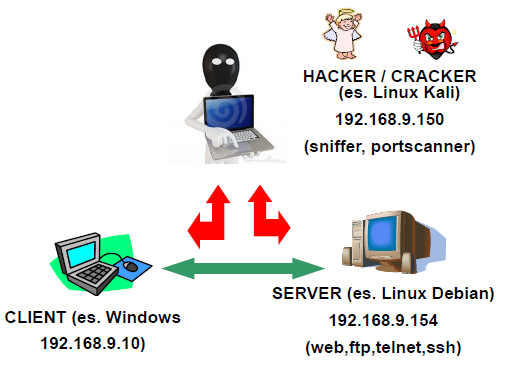
\includegraphics[width=0.8\textwidth]{immagini/Sniffer&portscanner.png}
    \caption*{Situazione tipica}
\end{figure}
Li vediamo in ambito \textbf{\emph{lecito}} (didattico, debug, risoluzione problemi, errori configurazione, ecc\dots).\
Esempi ``reali e/o pratici'':

\begin{itemize}
    \item sniffer:\ src/dst uguale server LAN laboratorio.
    \item sniffer:\ bittorrent e consumo banda notebook.
    \item sniffer/portscan:\ trojan o malware redirezione traffico uscita (web) o rete nascosta (botnet).
    \item portscan:\ installare un nuovo dispositivo (servizi attivi).
    \item sniffer/portscan:\ identificazione virus (es.\
          Conficker).
\end{itemize}

\begin{center}
    \textbf{Attenzione a cosa si fa!!}
\end{center}
\begin{itemize}
    \item Non si può attivare uno sniffer in una rete senza autorizzazione
          \begin{itemize}
              \item privacy, raccolta informazioni, normativa sul lavoro, ecc\dots
          \end{itemize}
    \item Non si può effettuare portscan liberamente contro qualsiasi obiettivo senza autorizzazione
          \begin{itemize}
              \item regolamento ISP, controlli \& IDS, risvolti legali, ecc\dots
          \end{itemize}
\end{itemize}

\section{Sniffer}

\subsubsection{Storia}

I programmi per il network tracing sono noti dalla fine degli anni '80.\
A quel tempo gli analizzatori per scopi commerciali non erano disponibili; il più famoso era il programma Sniffer, sviluppato da Network General.\
Il termine sniffing risale a tale programma.\


Sulle macchine Unix il programma tcpdump è stato sviluppato da Van Jacobsen, Leers e McCanne alla fine degli anni '80, questo programma e la libreria libpcap possono essere visti come i nonni di Wireshark.

All'inizio degli anni '90 erano disponibili molti analizzatori di pacchetti commerciali, la maggior parte di essi erano costosi e integrati nell'hardware.\


La situazione è cambiata alla fine degli anni '90 con lo sviluppo di ``Ethereal'' di Gerald Combs, questo programma è stato costruito sopra libpcap e la libreria GIMP Tool Kit (GTK), questo ha portato un analizzatore gratuito a molti sistemi operativi diversi.

\subsection{Cosa è uno sniffer?}

Uno \emph{sniffer} è un software per leggere ed analizzare il traffico di rete che arriva ad una certa macchina; si deve avere accesso alla rete locale.

Opera direttamente al livello di collegamento fisico della rete ethernet, quindi ai livelli 1 (fisico) e 2 (data link).\
È utile per scopi:
\begin{itemize}
    \item \textbf{leciti}:\ didattici, test, debug e monitoraggio (NIC guasta).
    \item \textbf{illeciti}:\ traffico non autorizzato, username/password, rootkit \& backdoor.
\end{itemize}
Si imposta l’interfaccia di rete in \textbf{\emph{modalità promiscua}} (cattura cioè anche il traffico non diretto alla propria scheda di rete):
\begin{itemize}
    \item ifconfig eth0 promisc
    \item ifconfig eth0 -promisc (ritorno modo funzionamento normale).
\end{itemize}
Deve essere eseguito con i privilegi di root (o amministratore).

\begin{figure}[H]
    \centering
    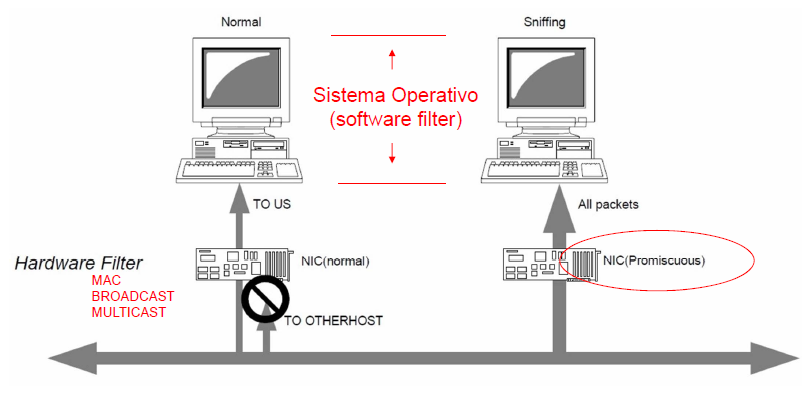
\includegraphics[width=\textwidth]{immagini/Promiscuous_mode.png}
    \caption*{Modalità promiscua}
\end{figure}

\begin{figure}[H]
    \centering
    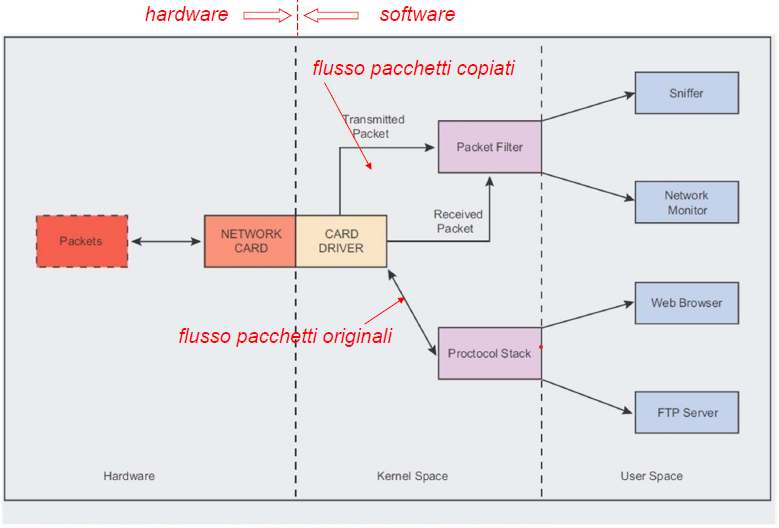
\includegraphics[width=0.8\textwidth]{immagini/Capture_process.png}
    \caption*{Elementi coinvolti nel processo di cattura}
\end{figure}
L’attività di sniffing (causa la copia dei pacchetti) è quindi onerosa dal punto di vista computazionale:

\begin{itemize}
    \item CPU
    \item memoria RAM
    \item spazio disco
    \item conseguente rallentamento attività di rete
\end{itemize}
Dipende dalla quantità di traffico da
analizzare:
\begin{itemize}
    \item possibile perdita di pacchetti (NIC o driver inadatti)
    \item Large Receive Offload (lro), Generic Receive Offload (gro)
          \begin{itemize}
              \item NIC riassembla i pacchetti prima di passarli al kernel
              \item problemi con alcuni sniffer evoluti (snort)
          \end{itemize}
\end{itemize}
Nell’ambito dello \emph{sniffing}, abbiamo dei problemi in ambienti di rete con gli \textbf{switch}.\
Uno \textbf{sniffer} deve poter ``vedere'' tutto il traffico che ci interessa.

\subsubsection{Switch Ethernet}

Ha un certo numero di porte Ethernet.\
Il traffico è veicolato \textbf{esclusivamente} fra le porte a cui sono connessi i dispositivi che lo generano e che devono riceverlo:
\begin{itemize}
    \item Sicurezza (proprio contro gli sniffer)
    \item Prestazioni (traffico esclusivamente tra mittente e destinatario)
\end{itemize}
Mano a mano che gli host generano traffico lo switch memorizza le associazioni ``MAC address source'' $\rightarrow$ ``porta''.\


Instrada i frame Ethernet esclusivamente verso la porta sulla quale lo switch ``vede'' il MAC address di destinazione.\
Replica del frame su tutte le porte (comportamento hub):
\begin{itemize}
    \item se il MAC address è quello di broadcast;
    \item se non è a lui noto.
\end{itemize}
\dots in una LAN ``\textbf{\emph{switchata}}'' esistono diverse soluzioni:
\begin{itemize}
    \item porta \textbf{MONITOR} o \textbf{SPAN} (\emph{Switch Port ANalyzer}) dove replicare il traffico delle porte interessate o tutto il traffico.
    \item un ``vecchio'' \textbf{HUB} (\emph{per reti non troppo veloci}).
    \item dispositivi \textbf{TAP} (\emph{Test Access Port}).
    \item \textbf{BRIDGE software}.
    \item \textbf{ARP cache Poisoning} (!!)
\end{itemize}
\begin{figure}[H]
    \centering
    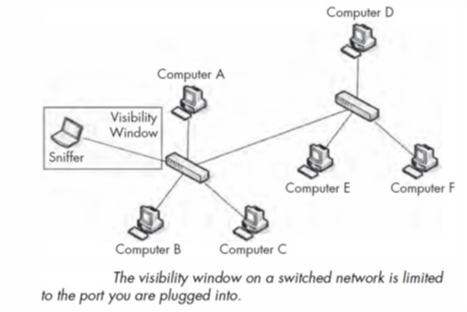
\includegraphics[width=0.6\textwidth]{immagini/sniffer_switch.png}
\end{figure}

\subsection{Come lavora uno sniffer?}

Il processo di packet-sniffing coinvolge hardware (NIC) \& software.\
Imposta la NIC in promiscuos mode; tutto il traffico viene catturato e passato al sistema operativo e alle applicazioni specifiche.\
Il funzionamento prevede 3 passaggi:
\begin{itemize}
    \item \emph{Raccolta}:\ sono raccolti i dati binary grezzi (raw).
    \item \emph{Conversione}:\ sono convertiti in forma leggibile (interpretabile), anche se solo a basso livello; molti tool a linea di comando si fermano qui (tcpdump).
    \item \emph{Analisi}:\ analisi approfondita ed elaborata dei dati raccolti; alcuni software evoluti agevolano l’analisi da parte dell’utente (wireshark).
\end{itemize}
In ambiente GNU/Linux si usano solitamente le librerie \textbf{libpcap} (\emph{Packet Capture}).\
In ambiente MS Windows le \emph{classiche} librerie \textbf{winpcap} o le \emph{nuove} \textbf{npcap}.

Si sfruttano le funzionalità chiamate \textbf{BPF} (Berkeley Packet Filter); permettono di specificare delle espressioni come filtro (\emph{poter selezionare solo il traffico di interesse}).\
Tali funzionalità sono fornite direttamente dalla libreria libpcap con sintassi generica (\emph{standard de-facto}); utilizzate con tutti gli sniffer (e anche molti IDS) che usano libpcap.\
Il file del traffico catturato (in formato .pcap) può quindi essere analizzato con software e strumenti diversi (tcpdump, wireshark, ecc).\
Il formato .pcap è di fatto uno standard.

\begin{figure}[H]
    \centering
    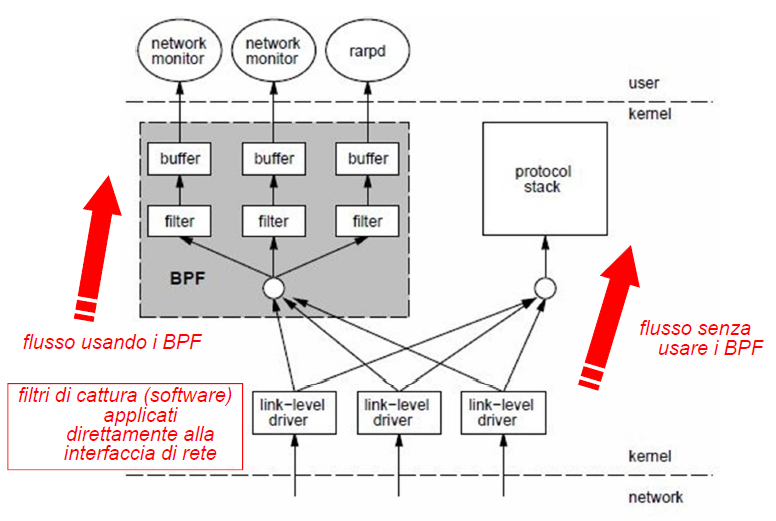
\includegraphics[width=0.7\textwidth]{immagini/BPF_overview.png}
    \caption*{BPF Overview}
\end{figure}

\begin{figure}[H]
    \centering
    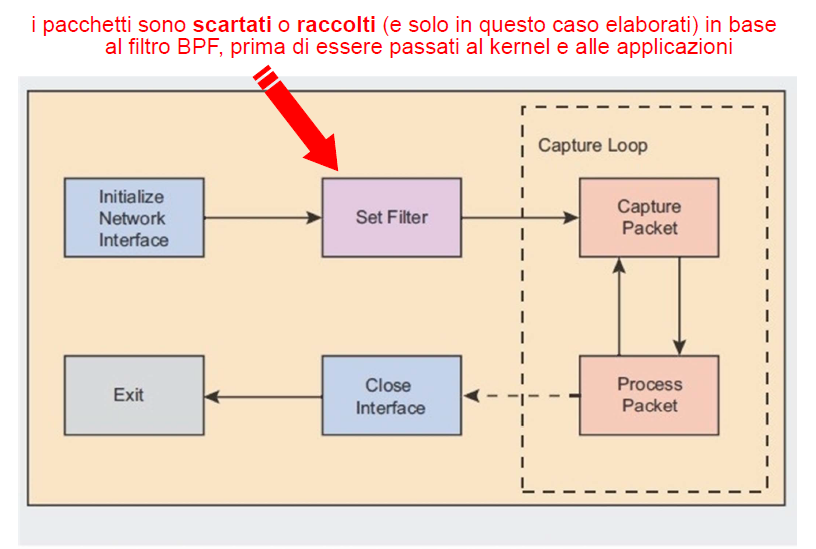
\includegraphics[width=0.9\textwidth]{immagini/pcap_flow.png}
    \caption*{Normal program flow of a pcap application}
\end{figure}

\subsubsection{Esempi di sniffer}

In ambiente GNU/Linux:
\begin{itemize}
    \item TCPDUMP
    \item suite WIRESHARK (TSHARK versione command line, DUMPCAP, EDITCAP)
    \item IPTRAF (network monitor)
    \item XPLICO (network forensic analysis tool)
    \item NGREP
    \item ETTERCAP (MiTM), NAST
    \item DSNIFF (password sniffer), P0F (fingerprint passivo)
    \item TCPKILL
    \item ETHERAPE (network monitor)
    \item NTOP (network monitor)
    \item SNORT (Network IDS)
\end{itemize}
In ambiente Microsoft Windows:
\begin{itemize}
    \item suite WIRESHARK (TSHARK versione command line, DUMPCAP, EDITCAP)
    \item WINDUMP (versione tcpdump per MS Windows)
    \item SATORI (fingerprint passivo)
    \item CAIN \& ABEL
    \item Microsoft MESSAGE ANALYZER (ex Microsoft NETWORK MONITOR):\ sfrutta driver a basso livello del Sistema Operativo MS Windows, spesso usato per sniffer WiFi $\rightarrow$ \textbf{dismesso/deprecato}
    \item RAWCAP, SMARTSNIFF (localhost,loopback)
\end{itemize}

\subsection{TCPDUMP}

\begin{itemize}
    \item In pratica è una interfaccia a riga di comando della libreria libpcap.\

    \item Permette di catturare il traffico di rete in tempo reale, di salvarlo su file (per una analisi successiva) e di rileggere file .pcap raccolti anche con software diversi.
\end{itemize}

\begin{table}[H]
    \centering
    \begin{tabular}{|l|m{28em}|}
        \hline
        Opzione  & Descrizione                                                                         \\\hline\hline
        -i iface & specifica un'interfaccia su cui ascoltare.                                          \\
        -w file  & scrive i pacchetti letti sul file \textbf{file}.                                    \\
        -r file  & legge i pacchetti dal file \textbf{file}.                                           \\
        -c count & legge esattamente \textbf{count} pacchetti.                                         \\
        -n       & non effettua la risoluzione degli indirizzi.                                        \\
        -p       & non porta l'interfaccia in modo promiscuo.                                          \\
        -t       & non stampa la temporizzazione dei pacchetti.                                        \\
        -v       & aumenta le informazioni stampate a video.                                           \\
        -q       & diminuisce le informazioni stampate a video.                                        \\
        -e       & stampa anche i dati relativi al protocollo di collegamento fisico (il MAC address). \\
        -F file  & usa il contenuto di \textbf{file} come filtro.                                      \\\hline
    \end{tabular}
\end{table}

\subsubsection{BPF (Berkley Packet Filter)}

Composti da quelle che si chiamano ``\emph{primitive}''; espressioni elementari che permettono di identificare una certa classe di traffico di rete.
\begin{center}
    \textbf{primitiva = qualificatore + identificatore}
\end{center}
Qualificatori:
\begin{itemize}
    \item \emph{di tipo}:\ host, net, port.
    \item \emph{di direzione}:\ src, dst, src or dst, src and dst.
    \item \emph{di protocollo}:\ ether, ip, ip6, arp, rarp, tcp, udp, icmp, \dots
\end{itemize}
TCPDUMP converte e compila ``al volo'' (\emph{runtime}) la sintassi BPF ad alto livello (primitive a livello utente) nel codice BPF a basso livello per la ``pseudo-machine'' (tcpdump -d).

Fondamentali in base a quantità di traffico (limitano dati da elaborare)
\begin{itemize}
    \item Security Onion
    \item Netsniff-NG (\emph{sniffer evoluto})
\end{itemize}

\begin{table}[H]
    \centering
    \begin{tabular}{|l|m{17em}|m{10em}|}
        \hline
        Qualifier & Description                                                     & Examples                       \\\hline \hline
        Type      & Identifies what the ID name or number refers to                 & host, net, port                \\
        Dir       & Specifies a transfer direction to or from the ID name or number & src, dst                       \\
        Proto     & Restricts the match to a particular protocol                    & ether, ip, tcp, udp, http, ftp \\\hline
    \end{tabular}
    \caption*{The BPF Qualifiers}

\end{table}
\begin{figure}[H]
    \centering
    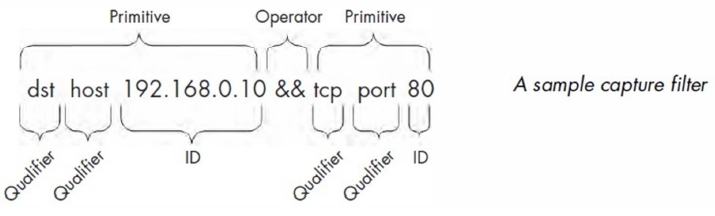
\includegraphics[width=0.7\textwidth]{immagini/capture_filter_ex.png}
\end{figure}

\subsubsection{Struttura di output di TCPDUMP}

L'output tcpdump fornisce per impostazione predefinita alcune informazioni di base su ciascun pacchetto.\
La formattazione di questo output varierà in base ai protocolli in uso, ma i formati più comuni sono:
\begin{itemize}
    \item TCP:

          [Timestamp] [Layer 3 Protocol] [Source IP].[Source Port]$>$[Destination IP].[Destination Port]:\ [TCP Flags], [TCP Sequence Number], [TCP Acknowledgment Number], [TCP Windows Size], [Data Length]
    \item UDP:

          [Timestamp] [Layer 3 Protocol] [Source IP].[Source Port]$>$[Destination IP].[Destination Port]:\ [Layer 4 Protocol], [Data Length]
\end{itemize}
Puoi forzare tcpdump a fornire più informazioni in questa riga di riepilogo aggiungendo il tag -v per aumentarne la verbosità.

\subsection{Wireshark}

Estremamente potente, dotato di interfaccia grafica che ne facilita l’utilizzo.\
Dispone di ``protocol dissector''; permetteno di effettuare
una ``dissezione'' (\emph{analisi}) dettagliata del traffico catturato.\
Permette di ricostruire il flusso di dati (stream) così da poter individuare i dati ``effettivamente'' catturati al livello di applicazione (email, pagine web, password, ecc\dots).

Crea statistiche e grafici dai dati elaborati.\
È possibile rileggere il traffico catturato in formato .pcap anche con strumenti diversi (es tcpdump).

Permette di usare i \textbf{filtri di cattura} BPF.\
Possiede dei \textbf{filtri di visualizzazione} per agevolare analisi.

È una suite di strumenti, esiste una versione testuale da linea di comando chiamato TSHARK.

\section{Port Scanner}

Software in grado di rilevare informazioni su un host (o una intera rete) e quali servizi sono attivi.\
Scansiona le porte (TCP e UDP) per identificare quali di esse sono utilizzate da un servizio.\
Può ``forzare'' a provocare certi tipi di risposta, al fine di raccogliere informazioni utili.

È uno strumento indispensabile per verificare in
maniera effettiva la \emph{propria} rete.\
Ê uno strumento di tipo attivo (a differenza di uno
sniffer).

In generale un port scanner genera traffico e ``confusione'' in una rete, quindi è potenzialmente identificabile.\
Usato per scopi \textbf{offensivi} (ricerca servizi vulnerabili
da attaccare), \textbf{indispensabile} per scopi di \textbf{difesa} (ricerca servizi vulnerabili o inutili da chiudere).

\subsubsection{Portsweep}

Tecnica di scansione simile al portscanning.\
Si effettua una scansione di uno o più host (o di una intera rete) alla ricerca della disponibilità di un singolo servizio (e/o una vulnerabilità) concentrandosi però su una singola porta.

Il portscannig, invece, effettua una scansione su diverse porte di diversi host (o una intera rete).\
Esempio:\ effettuare un portsweep degli host della nostra LAN sulla porta 3389 per individuarne versioni con problemi di sicurezza.
Le finalità sono le stesse del portscannig:
\begin{itemize}
    \item diagnostica
    \item attacco
\end{itemize}

\subsubsection{Individuazione/difesa}

La pratica del portscan è decisamente invasiva e può risultare ``pericolosa''; può essere identificata come un vero e proprio attacco informatico!!

La maggior parte dei sistemi di difesa prevedono dei metodi per identificarla; SNORT (uno dei Network IDS più utilizzati) prevede sia un preprocessore (sfportscan) che delle regole costruite ``ad-hoc'' al fine di identificare i portscan.

\subsection{NMAP}

È il più utilizzato per eseguire portscanning (comunque ne esistono altri).\
Estremamente flessibile ed ottimizzato:
\begin{itemize}
    \item esegue portscan più o meno invasivi e/o più o meno identificabili.
    \item rileva la presenza e tipologia di firewall.
    \item identifica caratteristiche e versione del sistema operativo e dei servizi remoti (fingerprint attivo).
    \item presenta report completi e dettagliati.
\end{itemize}
Prevede un proprio linguaggio di scripting (Nmap Scripting Engine - NSE) per automatizzare e migliorare le analisi.\
Scansiona intere reti in tempi brevissimi.\
Dotato anche di interfaccia grafica (ZENMAP).

\subsubsection{Funzionamento}

Per usufruire di tutte le sue funzionalità, si deve eseguire come amministratore (l’unico che può ``forgiare'' pacchetti ad-hoc).\
Si basa sul tipo di risposte ricevute previste dagli standard dei protocolli di rete.

Crea ad-hoc delle richieste (non sempre ``formalmente'' corrette) per generare delle risposte previste e predefinite.\
Sfrutta le peculiarità dei protocolli di rete (si addentra nei ``meandri'' del loro funzionamento).

Dalle risposte ricevute (e dal confronto con i suoi db interni) identifica tutta una serie di caratteristiche del sistema bersaglio.

Per default (\emph{escluso il Connect Scan -sT}) usa pacchetti minimali e non invasivi, quindi senza dati (vuoti):
\begin{itemize}
    \item il portscanning di solito ``non fa danni'' (a meno di bug del servizio remoto\dots); è la pratica del portscanning ritenuta dannosa/offensiva!
\end{itemize}
Cerca in questo modo di non lasciare tracce:
\begin{itemize}
    \item nei log dei servizi remoti.
    \item nei log del sistema operativo remoto:
          \begin{itemize}
              \item un pacchetto ``strano'' generato da nmap può causare un errore nello stack di rete remoto che può essere identificato:\ \emph{``May 15 11:28:57 server proftpd[3324] server:\ Fatal:\ unable to open incoming connection:\ Transport endpoint is not connected''}
          \end{itemize}
    \item è comunque impossibile prevedere tutte le possibili implementazioni dei servizi remoti (specialmente nel caso di servizi in UDP, dove i controlli sono demandati alla applicazione), quindi a volte qualche traccia risulta \dots
\end{itemize}

\subsubsection{Firewall}

\begin{itemize}
    \item DROP:\ il pacchetto ricevuto viene silenziosamente scartato (non viene inviata nessuna risposta al client).
    \item REJECT:\ il pacchetto ricevuto viene scartato ma viene prodotta una risposta verso il client:
          \begin{itemize}
              \item TCP:\ invio pacchetto RST.
              \item UDP:\ invio pacchetto ICMP ``Port Unreachable''.
              \item possibilità di personalizzare il tipo di risposta mediante la direttiva --reject-with \emph{TIPO\_PACCHETTO} (\emph{icmp-net-unreachable, icmp-portunreachable, icmp-proto-unreachable, ecc}\dots).
          \end{itemize}
\end{itemize}

\subsubsection{Portscan di default}

\begin{itemize}
    \item Come utente non privilegiato:CONNECT SCAN (-sT)
    \item Come utente amministratore (root):\ SYN SCAN (chiamato anche semi apertura o half-open) (-sS)
    \item A seguito della scansione, le porte possono risultare:
          \begin{itemize}
              \item OPEN:\ servizio attivo sulla porta ed accessibile.
              \item CLOSED:\ nessun servizio sulla porta.
              \item FILTERED:\ può essere attivo un servizio sulla porta ma la comunicazione è bloccata e non si è in grado di capire se OPEN o CLOSED.
              \item UNFILTERED:\ nel solo caso di TCP ACK Scan (-sA).
              \item OPEN| FILTERED:\ situazione indeterminata (nel caso di scanUDP, IP, protocol, FIN, NULL e Xmas).
              \item CLOSED|FILTERED:\ situazione indeterminata (nel solo caso di TCP Idle Scan -sI).
          \end{itemize}
\end{itemize}

\subsubsection{Connect scan (-sT)}

Effettua una serie di normali connessioni TCP (SYN$\rightarrow$, $\leftarrow$ SYN{\slash}ACK, ACK$\rightarrow$).\
Funzionamento:
\begin{itemize}
    \item porta aperta:\ si riceve una risposta dal demone attivo con successiva chiusura della connessione; porta OPEN.
    \item porta chiusa (senza firewall):\ si riceve in risposta una connessione abortita (invio di RST in risposta a connessione su porta chiusa, come previsto dallo stack TCP/IP); porta CLOSED.
    \item con firewall (DROP):\ non si riceve risposta, i pacchetti sono scartati dal firewall, quindi si ha un time out; porta FILTERED.
\end{itemize}
Questa modalità è facilmente individuabile dai log, causa apertura/chiusura di porte senza traffico effettivo.\
La dimensione del pacchetto SYN è quella normale; ci sono dati contenuti in ``options'' [mss, wscale, ecc\dots]

\subsubsection{SYN scan (-sS)}

È la modalità utilizzata di default (chiamata anche \emph{stealth mode}).\
Esegue la prima parte dell’apertura (semi-apertura) della connessione TCP (non completa la connessione iniziale, manca ACK finale dal client).\
Invio di un pacchetto SYN \textbf{\emph{creato da nmap}}:
\begin{itemize}
    \item porta aperta:\ si riceve in risposta SYN+ACK; OPEN
    \item porta chiusa:\ si riceve in risposta un RST/ACK; CLOSED
    \item Firewall (DROP):\ nessuna risposta; FILTERED
\end{itemize}
Non serve concludere la connessione da parte di nmap!

Se la porta è aperta e ricevo un SYN+ACK dal target, lo stack TCP del sistema dove si esegue nmap risponde con un RST poiché il SYN+ACK ricevuto dal target non corrisponde a nessun SYN iniziale iniziato da un processo del sistema.

NMAP usa ciò che si chiama ``\emph{RAW SOCKET}''.\
Crea artificialmente il SYN, invece di usare la systemcall \emph{connect()} del kernel (quindi, a differenza di -sT).\
Il pacchetto SYN (RAW SOCKET) creato da nmap è diverso (più piccolo) di un normale SYN; mancano dati in options (è
presente solo [mss]).

Non completando la connessione, il target in questo modo non si accorge di niente; questa scansione non lascia tracce sul target.\
Rilevabile però dalla maggior parte dei tool di sorveglianza (SNORT, Scanlogd, synlogger, ecc) e può essere bloccato da firewall che filtrano le nuove connessioni (SYN).

\subsubsection{Version detection (-sV)}

Tenta una connessione ai servizi trovati per determinarne la versione, in base alle risposte di questi ultimi:
\begin{itemize}
    \item banner ricevuto dal demone del servizio.
    \item altre informazioni distintive del servizio in ascolto.
\end{itemize}
Confronta le risposte con l’elenco presente nel file /usr/share/map/nmap-service-probes.

Nmap tenta la connessione ed aspetta circa 5 secondi una qualche risposta (tempo di rispondere se il servizio fosse impegnato).\
Può essere ``ingannato'' per eludere proprio i portscan:
\begin{itemize}
    \item modificando banner magari con quello di una versione senza bug.
    \item cambiando la porta di default (telnet sulla porta 22).
\end{itemize}
Nei log, questa scansione può lasciare tracce:
\begin{itemize}
    \item se è attivo sshd, in auth.log ritroviamo qualcosa tipo:\
          \begin{flushleft}
              ``\texttt{server sshd[2022]:\ Did not receive identification string from 192.168.9.151}''
          \end{flushleft}
    \item se è attivo un smtp server (es postfix), in mail.log ritroviamo qualcosa tipo:
          \begin{itemize}
              \item ``Apr 19 14:12:56 server postfix/smtpd[2463]:\ connect from unknown[192.168.9.151]''
              \item ``Apr 19 14:12:56 server postfix/smtpd[2463]:\ lost connection after CONNECT from unknown[192.168.9.151]''
              \item ``Apr 19 14:12:56 server postfix/smtpd[2463]:\ disconnect from unknown[192.168.9.151]''
          \end{itemize}
\end{itemize}
Potrebbe mandare in crash il servizio remoto (\emph{se non progettato correttamente\dots}).\
Generalmente viene individuata anche dai sistemi IDS.


\subsubsection{TCP/IP Fingerprint (-O)}

Analizzando le risposte ad una serie di pacchetti di prova, si cercano di identificare caratteristiche dello stack TCP/IP del TARGET, basandosi su una serie di risposte note (/usr/share/nmap/nmap-os-db).\


\textbf{\emph{Identifica il sistema operativo}}, in base alla TCP/IP fingerprint caratteristica di ogni OS.\
Identifica la predicibilità dei numeri di sequenza dello stack TCP (misura la difficoltà di creare pacchetti ad-hoc per inserirsi in una connessione).

\textbf{\emph{Identifica uptime}} del sistema.

\begin{figure}[H]
    \centering
    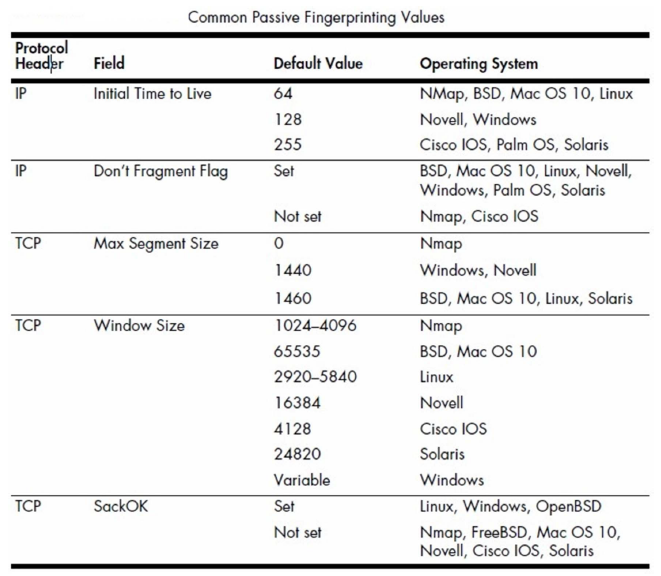
\includegraphics[width=0.8\textwidth]{immagini/Fingerprint_values.png}
\end{figure}

\begin{figure}[H]
    \centering
    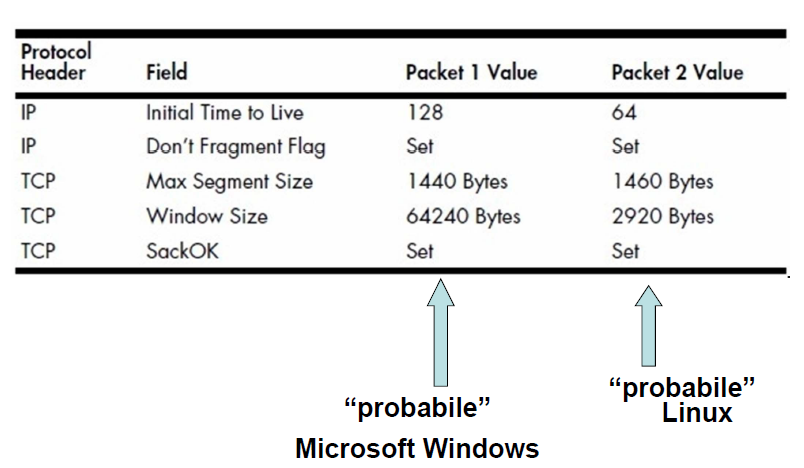
\includegraphics[width=0.8\textwidth]{immagini/Fingerprint_confronto.png}
    \caption*{Esempio di OS Fingerprint a confronto}
\end{figure}

\subsubsection{Curiosità}

È possibile riconoscere (con ragionevole certezza) il sistema operativo remoto molto banalmente osservando le risposte ad un semplice ping.\
Osservando il campo TTL della risposta:
\begin{itemize}
    \item Sistemi Microsoft:\ TTL inizia da 128
    \item Sistemi Linux:\ TTL inizia da 64
    \item Sistemi BSD:\ TTL inizia da 128
\end{itemize}
Non è casuale che i sistemi Microsoft e BSD forniscano le stesse tempistiche:\ Microsoft, ha costruito il proprio stack TCP/IP riprendendolo a piene mani dai sistemi BSD\dots

\chapter{Cifrari storici}

Lo scopo dei cifrari storici era quello di consentire comunicazioni ``sicure'' tra poche persone, ma sono stati tutti forzati.\
La cifratura e la decifrazioni erano realizzate con carta e penna, e i messaggi da cifrare erano frasi di senso compiuto in linguaggio naturale.\

I cifrari storici seguivano i \textbf{principi di Bacone} (XIII secolo):
\begin{enumerate}
    \item Le funzioni $C$ e $D$ devono essere \textit{facili da calcolare}.
    \item È \textbf{impossibile} ricavare la $D$ se la $C$ non è nota.
    \item Il crittogramma $c=C(m)$ deve apparire ``\textit{innocente}''.
\end{enumerate}

\section{Cifrario di Cesare}

È il più antico cifrario di concezione moderna.\
Il crittogramma $c$ è ottenuto dal messaggio in chiaro $m$ sostituendo ogni lettera di $m$ con quella tre posizioni più avanti nell'alfabeto.\

Si noti che non vi è alcuna chiave segreta:\ la segretezza dipende dalla sola conoscenza del metodo, scoprire il metodo significava comprometterne irrimediabilmente l'impiego.\
Per questi motivi, il cifrario di Cesare era destinato all'\textbf{uso ristretto} di un gruppo di conoscenti.\

Può essere trasformato aumentandone la sicurezza:\ invece di ruotare l'alfabeto di tre posizioni, è possibile ruotarlo di una quantità arbitraria $k$, $1\leq k\leq 25$ (26 lascia inalterato il messaggio); in questo caso $k$ è la \textbf{chiave segreta} del cifrario.\

\subsubsection{Formulazione matematica}

$pos(X)$ è la posizione della lettera $X$ nell'alfabeto e $k$ è la chiave, $1\leq k \leq 25$.\

\begin{itemize}
    \item Cifratura di $X$:\ lettera $Y$ tale che $pos(Y) = (pos(X) + k)\ \mathit{mod}\ 26$
    \item Decifrazione di $Y$:\ lettera $X$ tale che $pos(X) = (pos(Y) - k)\ \mathit{mod}\ 26$
\end{itemize}

\subsubsection{Realizzazione fisica}

Due dischi concentrici

\begin{itemize}
    \item disco interno:\ lettere dell'alfabeto in chiaro;
    \item disco esterno:\ lettere cifrate.\
\end{itemize}

\noindent Si pone una lettera del disco interno in corrispondenza con una lettera del disco esterno, in accordo con $k$.\
Ovviamente, tutte le altre lettere combaceranno con le corrispondenti lettere cifrate.

\subsubsection{Crittoanalisi}

Se si conosce la struttura del cifrario, si possono applicare in breve tutte le chiavi possibili (25) a un crittogramma per decifrarlo e scoprire contemporaneamente la chiave segreta:\ cifrario inutilizzabile a fini crittografici.\

\subsubsection{Osservazioni}

Gode della proprietà commutativa:\ data una sequenza di chiavi e di operazioni di cifratura e decifrazione, l'ordine delle operazioni può essere permutato arbitrariamente senza modificarne il crittogramma finale.\

Comporre più cifrari non aumenta la sicurezza del sistema:\ date due chiavi $k_1, k_2$ e una sequenza $s$
\[C(C(s,k_2), k_1) = C (s, k_1 + k_2)\]
\[D(D(s,k_2), k_1) = D (s, k_1 + k_2)\]
una sequenza di operazioni di cifratura e decifrazione può essere ridotta ad una sola operazione di cifratura o decifrazione.\

\section{Classificazione dei cifrari storici}

Il cifrario di Cesare è detto \textbf{a sostituzione}:\ sostituisce ogni lettera del messaggio in chiaro con una o più lettere dell'alfabeto secondo una regola prefissata.\
Si possono distinguere due classificazioni
\begin{itemize}
    \item Sostituzione \textbf{monoalfabetica}:\ alla stessa lettera del messaggio corrisponde sempre una stessa lettera nel crittogramma (e.g.\ cifrario di Cesare).\ Nei cifrari di questo tipo è possibile impiegare funzioni di cifratura più complesse della semplice addizione e sottrazione in modulo.\ Questo rende lo spazio delle chiavi più ampio ma la loro sicurezza rimane comunque molto modesta.\ Sono stati tutti forzati grazie alla crittoanalisi statistica che studia l'ordine, la frequenza e la posizione con cui si presentano parole e lettere.\
    \item Sostituzione \textbf{polialfabetica}:\ alla stessa lettera del messaggio corrisponde una lettera scelta in un insieme di lettere possibili secondo una regola opportuna, ad esempio, a seconda della posizione della lettera da sostituire oppure del contesto in cui essa appare nel messaggio.
\end{itemize}

\noindent Esistono anche i cifrari \textbf{a trasposizione} che permutano le lettere del messaggio in chiaro secondo una regola prefissata.\

\subsection{Cifrari a sostituzione monoalfabetica}

\subsubsection{Cifrario affine}

\textbf{Cifratura}:\ una lettera in chiaro $X$ viene sostituita con la lettera cifrata $Y$ che occupa nell'alfabeto la posizione
\[\mathit{pos}(Y) = (a \cdot \mathit{pos}(X) + b)\ \mathit{mod}\ 26\]
$ k = \langle a,b\rangle$:\ chiave segreta del cifrario.

\vspace{12pt}
\noindent\textbf{Decifrazione}:\
\[\mathit{pos}(X) = a^{-1} \cdot (\mathit{pos}(Y) - b)\ \mathit{mod}\ 26\]
$a^{-1}$:\ è l'inverso di $a$ modulo 26:
\[a \cdot a^{-1} = 1\ \mathit{mod}\ 26\]

\noindent L'inverso di un intero $a$ modulo $m$ \textbf{esiste ed è unico} se e solo se \[\mathrm{MCD}(a, m) = 1\]
Si tratta di un vincolo forte sulla definizione della chiave:\ se $\mathrm{MCD}(a, m) \neq 1$, la \textit{funzione di cifratura non è iniettiva e la decifrazione diventa impossibile}.\

\vspace{12pt}
\noindent$a$ e 26 devono essere co-primi
\begin{itemize}
    \item i fattori primi di 26 sono 2 e 13
    \item $a$ può assumere qualsiasi valore dispari tra 1 e 25, ad eccezione di 13 (12 valori possibili)
\end{itemize}
$b$ può essere scelta liberamente tra 0 e 25, dunque può assumere 26 valori.
\vspace{12pt}

\noindent Le chiavi legittime sono tutte le possibili $\langle a,b \rangle$, in totale $12 \times 26 = 312$ chiavi (troppo poche); in realtà sono 311 (la coppia $\langle 1,0 \rangle$ lascia inalterato il messaggio).\

Se la segretezza dipende unicamente dalla chiave, il numero delle chiavi deve essere così grande da essere praticamente immune ad ogni tentativo di provarle tutte.\
La chiave segreta deve essere scelta in modo (possibilmente) casuale da un insieme molto grande.\

In un cifrario a sostituzione monoalfabetica è possibile aumentare la cardinalità delle chiavi prendendo una permutazione arbitraria dell'alfabeto come chiave:
\begin{center}
    lettera in chiaro di posizione $i$ $\Rightarrow$ lettera di posizione $i$ nella permutazione.
\end{center}

\noindent In questo caso, lo spazio delle chiavi \textbf{aumenta enormemente}:\ abbiamo una chiave fatta di 26 lettere invece dei due numeri interi del cifrario affine; di conseguenza, lo spazio delle chiavi è esteso a $26! - 1\ (\sim 4\cdot 10^{26})$ chiavi e quindi è vasto e inesplorabile con metodi esaurienti.\
Tuttavia, il cifrario non è ancora sicuro:\ il sistema è attaccabile facilmente con un'\textbf{analisi statistica} sulla frequenza dei caratteri.\

\subsection{Cifrario a sostituzione polialfabetica}

\subsubsection{Archivio cifrato di Augusto}

Augusto manteneva il proprio archivio cifrato:\ i documenti erano scritti in numeri, non in lettere.\
Fu svelato dall'imperatore Claudio circa 30 anni dopo la sua morte.\

Augusto scriveva i suoi documenti in greco, poi metteva in corrispondenza la sequenza di lettere del documento con la sequenza di lettere del primo libro dell'Iliade; dopodiché, sostituiva ogni lettera del documento con il numero che indicava la distanza, nell'alfabeto greco, di tale lettera con quella in pari posizione dell'Iliade.\

\vspace{12pt}
\noindent Esempio:
\begin{itemize}
    \item lettera in posizione $i$-esima nel documento:\ $\alpha$
    \item lettera in posizione $i$-esima nell'Iliade:\ $\varepsilon$
    \item carattere in posizione $I$-esima nel crittogramma:\ 4 (distanza fra $\alpha$ e $\varepsilon$)
\end{itemize}

\noindent\textbf{Osservazioni}:
\begin{itemize}
    \item cifrario difficile da forzare se la chiave è lunghissima;
    \item utilizzato nella seconda guerra mondiale prendendo come chiave una pagina prefissata di un libro e cambiandola di giorno in giorno;
    \item lo svantaggio è che la chiave va messa per iscritto e inviata al destinatario (nel caso in cui ci sia).
\end{itemize}

\subsubsection{Cifrario di Leon Battista Alberti}

Disco di Leon Battista Alberti (XV secolo):\
\begin{itemize}
    \item \textbf{alfabeto esterno}:\ lettere (alcune) e numeri, per formulare il messaggio.
    \item \textbf{alfabeto interno}:\ più ricco, disposto in modo arbitrario (e diverso per ogni coppia di utenti), per costruire il crittogramma.
\end{itemize}

\noindent L'allineamento iniziale dei dischi avviene prima e in segreto.\
I successivi allineamenti vengono scoperti dal destinatario mano a mano che decifra (corrispondenza con un numero).

\subsubsection{Metodo ``indice mobile''}

In questo metodo si usano sempre i dischi dell'Alberti ma si usa una tecnica particolare:\ quando si inserisce il numero $n$, che di norma rappresenterebbe un cambio di chiave, qui indica che dopo $n$ caratteri la chiave verrà cambiata.\

\vspace{12pt}
\noindent\textbf{Osservazioni}:
\begin{itemize}
    \item si cambia chiave ogni volta che si incontra un carattere speciale;
    \item inserendo  spesso i caratteri speciali (scartati nel messaggio ricostruito) il cifrario è difficile da attaccare;
    \item il continuo cambio di chiave rende inutili gli attacchi basati sulla frequenza dei caratteri.\
\end{itemize}
La \textbf{Macchina Enigma} (1918) è un'estensione elettromeccanica del cifrario di Alberti.\

\subsubsection{Cifrario di Vigenère (1586)}

La chiave è corta e ripetuta ciclicamente.\
Ogni lettera della chiave indica una \textit{traslazione della corrispondente lettera del testo}.

\textbf{Cifratura}:\ si dispongono $m$ e $k$ su due righe adiacenti, allineando le lettere in verticale (se $k$ è più corta di $m$, la chiave si ricopia più volte).\
Ogni lettera $X$ del messaggio in chiaro risulta allineata ad una lettera $Y$ della chiave.\
La $X$ viene sostituita nel crittogramma con la lettera che si trova nella cella di $T$ all'incrocio tra la riga che inizia con $X$ e la colonna che inizia con $Y$.\

Risulta essere un cifrario simmetrico, perciò necessita che le chiavi siano scambiate privatamente fra mittente e destinatario.\
La sicurezza del metodo è influenzata dalla lunghezza della chiave.\
Se la chiave contiene $h$ caratteri, le apparizioni della stessa lettera distanti un multiplo di $h$ nel messaggio si sovrappongono alla stessa lettera della chiave, quindi sono \textbf{trasformate nella stessa lettera cifrata}.\

Per ogni intero positivo $i \leq h$ si costruisce un sottomessaggio $m[i]$ formato dalle lettere di $m$ che occupano le posizioni $i, i+h, i+2h,\dots$
In ciascuno di tali sottomessaggi tutte le lettere sono allineate con la stessa lettera della chiave.\
Il messaggio decomposto in $h$ sottomessaggi, ciascuno dei quali è di fatto \textbf{cifrato con un metodo monoalfabetico}.\
I cifrari polialfabetici non sono dunque tanto più potenti dei monoalfabetici se le chiavi non sono molto lunghe.\

\subsubsection{One-Time Pad (1917)}

Se estendiamo il metodo di Vigenère impiegando una chiave \textit{lunga come il testo, casuale e non riutilizzabile}, il cifrario diviene \textbf{inattaccabile}:\ non può essere decifrato senza conoscere la chiave.\
È il caso di \textbf{One-Time Pad} che impiega un codice binario per messaggi e chiavi:\ fu usato nella \textit{Hot Line} per le comunicazioni tra la Casa Bianca e il Cremlino a partire dal 1967.\

Tuttavia, se la chiave è lunga quanto il messaggio, non può essere riutilizzata e necessita di essere scambiata fra i due estremi in maniera privata, tanto vale scambiarsi il messaggio.\
Difatti, il grosso problema di questi cifrari è proprio la lunghezza della chiave.

\subsection{Cifrari a trasposizione}

\textbf{Idea di base}:\ eliminare qualsiasi struttura linguistica presente nel crittogramma \textit{permutando le lettere del messaggio in chiaro} e inserendone eventualmente altre che vengono ignorate nella decifrazione.\

\subsubsection{Cifrario a permutazione semplice}

La chiave è costituita da un intero $h$ e da una permutazione $\pi$ degli interi $\{1,2,\dots,h\}$.\
Si suddivide il messaggio $m$ in blocchi di $h$ lettere e si permutano le lettere di ciascun blocco secondo $\pi$.\
Se la lunghezza di $m$ non è divisibile per $h$, si aggiungono alla fine delle lettere qualsiasi (\textit{padding}) che partecipano alla trasposizione, ma sono ignorate dal destinatario perché la decifrazione le riporta alle fine del messaggio.\

\textbf{Osservazione}:\ il numero delle chiavi è
\[h!-1\]
$h$ non è fissato; tanto maggiore è $h$, tanto più difficile è impostare un attacco esauriente.\
Al crescere di $h$, cresce anche la difficoltà di ricordare la chiave $\pi$.\

\subsubsection{Cifrario a permutazione di colonne}

$k = \langle c,r,\pi\rangle$
\begin{itemize}
    \item $c$ e $r$ denotano il numero di colonne e di righe di una tabella di lavoro $T$.\
    \item $\pi$:\ permutazione degli interi $\{1,2,\dots,c\}$.\
\end{itemize}

\noindent Il messaggio $m$ viene decomposto in blocchi $m_1,m_2,\dots$ di $c \times r$ caratteri ciascuno.\
Per cifrare il messaggio, i caratteri sono distribuiti tra le celle di $T$ in modo regolare, scrivendoli per righe dall'alto verso il basso; in seguito le colonne di T sono \textit{permutate} secondo $\pi$.\
Per cifrare il blocco $m_{i+1}$, $T$ viene azzerata e il procedimento si ripete.\

Il numero di chiavi è teoricamente esponenziale nella lunghezza del messaggio, non essendoci vincoli sulla scelta di $r$ e $c$.\

\subsection{Cifrari a griglia}

Progenitore:\ \textbf{cifrario di Richelieu}.\

Il crittogramma può essere celato in un libro qualsiasi e la chiave è data da una scheda perforata e dall'indicazione di una pagina del libro; la decifrazione consiste nel sovrapporre la scheda alla pagina:\ le lettere visibili attraverso la perforazione costituiscono il messaggio in chiaro.\

\subsubsection{Variante}

La chiave segreta è una griglia quadrata di dimensione $q \times q$, con $q$ pari.\
$s = \frac{q^2}{4}$ celle della griglia (un quarto del totale) sono trasparenti, le altre opache.\

Si scrivono i primi $s$ caratteri del messaggio, nelle posizioni corrispondenti alle celle trasparenti.\
La griglia viene routata tre volte di 90 gradi in senso orario e si ripete per ogni rotazione l'operazione di scrittura di tre successivi gruppi di $s$ caratteri.\
Alla fine del processo si fa un \textit{merge} delle tabelle.\

\begin{itemize}
    \item La griglia deve essere costruita in modo che le posizioni corrispondenti alle celle trasparenti non si sovrappongono mai nelle quattro rotazioni.\
    \item Se la lungheza del messaggio è minore di $4s$, le posizioni della pagina $P$ rimaste vuote si riempiono con caratteri scelti a caso.\
    \item Se la lunghezza del messaggio è maggiore di $4s$, il messaggio viene decomposto in blocchi di $4s$ caratteri ciascuno, e ogni blocco è cifrato indipendentemente dagli altri.
    \item La decifrazione di $P$ è eseguita sovrapponendovi quattro volte la griglia.
\end{itemize}

\noindent Le possibili chiavi sono quante sono le griglie $G= 4^s$.\
Con $q = 6$ si avrebbero $4^9 \approx 260000$ griglie possibili e per $q=13, G=d^{36}$ avremmo un numero sufficiente a porre il cifrario al riparo da un attacco esauriente.\

Il motivo per cui il numero di griglie è esattamente $4^s$ è da ricercare nella costruzione stessa della griglia:\ quando viene costruita una griglia si sceglie la prima cella (da lasciare trasparente) in maniera casuale, di modo che nelle tre successive rotazioni di 90 gradi non ricopra mai lo stesso punto.\

\section{Crittoanalisi statistica}

La sicurezza di un cifrario è legata alla dimensione dello spazio delle chiavi:\ uno spazio delle chiavi vasto (inesplorabile in tempo polinomiale) garantisce protezione da attacchi a forza bruta.\

I cifrari storici sono stati violati con un attacco statistico di tipo \textit{cipher text} (il crittoanalista ha a disposizione solo il crittogramma).\
L'impiego del metodo si fa risalire in Europa alla metà del XIX secolo, quando si scoprì come violare il cifrario di Vigenère, considerato assolutamente sicuro da 300 anni.\

Nell'ambito della crittoanalisi statistica, si suppone che il crittoanalista conosca:\

\begin{itemize}
    \item metodo impiegato per la cifratura/decifrazione;
    \item linguaggio naturale in cui è stato scritto il messaggio;
    \item si ammette che il messaggio sia sufficientemente lungo per poter rilevare alcuni dati statistici sui caratteri che compongono il crittogramma.\
\end{itemize}

\noindent La \textbf{crittoanalisi statistica} si basa sulla \textit{frequenza con cui appaiono in media le varie lettere dell'alfabeto}.\
Dati simili sono noti per le frequenze di \textbf{digrammi} (gruppi di due lettere consecutive), \textbf{trigrammi} (gruppi di tre lettere consecutive), e così via (\textbf{q-grammi}).\

\subsection{Attacco:\ sostituzione monoalfabetica}

Quando si usa la crittoanalisi per decifrare un crittogramma generato con sostituzione monoalfabetica, si esegue una \textbf{prima ipotesi di decifrazione}:
\begin{itemize}
    \item $y$ nel crittogramma corrisponde a $x$ nel messaggio,
    \item $\mathit{frequenza}(y) \approx \mathit{frequenza}(x)$.
\end{itemize}
Perciò, si confrontano le frequenze delle lettere e si provano alcune permutazione tra lettere con frequenze assai prossime:\ la A e la E compaiono nel 12\% dei casi e nel crittogramma c'è una lettera che compare nel 12\% circa dei casi, quindi si prova a sostituire la A e la E al posto di quella lettera e si controlla se la sostituzione ha un senso compiuto.

\subsubsection{Cifrari affini}

È sufficiente individuare due coppie di lettere corrispondenti con cui impostare un sistema di due equazioni nelle due incognite $a$ e $b$ che formano la \textbf{chiave segreta}.\
Risolvere il sistema è sempre possibile perché $a$ è invertibile.\

Se si tratta di una \textbf{cifrario completo} (cioè quando l'alfabeto viene messo in corrispondenza con una permutazione qualunque delle $26!$ che si possono costruire), allora si associano le lettere in base alle frequenze:\ le associazioni possono raffinare controllando i digrammi più frequenti.\
In genere a questo punto il cifrario è completamente svelato; altrimenti si passa ai trigrammi e così via.\

\subsection{Attacco:\ sostituzione polialfabetica}

La decifrazione è più difficile in questo caso:\ se si costruisce l'istogramma delle frequenze delle lettere del crittogramma, il risultato è generalmente piatto dato che non vi sono corrispondenze dirette fisse che rispettano il linguaggio.\

\subsubsection{Cifrario di Vigenère}

Ogni lettera $y$ del crittogramma dipende da una coppia di lettere $\langle x, k\rangle$ provenienti dal messaggio in chiaro e dalla chiave (si altera la frequenza delle lettere del crittogramma).\

La debolezza risiede nella chiave unica e ripetuta più volte:\ con una chiave di $h$ caratteri è possibile decomporre il crittogramma in varie sottosequenze lunghe $h$, ciascuna ottenuta per sostituzione monoalfabetica.\
L'unico problema è scoprire il valore di $h$:\ per farlo si sfrutta il fatto che i messaggi contengono quasi sicuramente gruppi di lettere adiacenti ripetuti più volte (trigrammi più frequenti nella lingua, parole a cui il testo si riferisce).\
Sostanzialmente le apparizioni della stessa sottosequenza allineate con la stessa porzione della chiave sono trasformate nel crittogramma in sottosequenze identiche.\
Quindi si cercano nel crittogramma coppie di posizioni $p_1,p_2$ in cui iniziano sottosequenze identiche e a questo punto è molto probabile che $p_2-p_1$ sia la lunghezza $h$ della chiave o un suo multiplo.\

\subsubsection{Cifrario di Alberti}

È immune da questi attacchi se la chiave viene cambiata spesso evitando pattern ripetitivi.\
Mantenere a lungo una chiave mette a rischio il cifrario perché in quel tratto la sostituzione è monoalfabetica.\

\subsection{Attacco:\ cifrari a trasposizione}
Nei crittogrammi generati con questi cifrari, le lettere del crittogramma sono una permutazione delle lettere del messaggio, perciò, eseguire un attacco che si basa sulla statistica andrebbe a generare degli istogrammi che sono identici a quelli generati dagli studi di un determinato linguaggio.\
Per forzare i cifrari a trasposizione semplice si sfruttano i \textit{q-grammi}:\ si divide il crittogramma in porzioni di lunghezza $h$ e in ciascuna si cercano i gruppi di $q$ lettere che formano i \textit{q-grammi} più diffusi nel linguaggio (non saranno adiacenti); se un gruppo deriva effettivamente da un \textit{q-gramma}, si scopre parte della permutazione.

\subsection{Conclusione}

La rilevazione delle frequenze delle singole lettere del crittogramma è un potente indizio per discernere tra i vari tipi di cifrario

\begin{itemize}
    \item nei cifrari a trasposizione l'istogramma delle frequenze coincide approssimativamente con quello proprio del linguaggio;
    \item nei cifrari a sostituzione monoalfabetica i due istogrammi coincidono a meno di una permutazione delle lettere;
    \item nei cifrari a sostituzione polialfabetica, l'istogramma del crittogramma è assai più piatto di quello del linguaggio (le frequenze delle lettere variano meno).
\end{itemize}

\section{La macchina Enigma}

Prima evoluzione verso sistemi automatizzati:\ si tratta di un'evoluzione elet\-tro-meccanica del cifrario di Alberti.\
Occupa un ruolo fondamentale nella storia recente (II guerra mondiale) e molti studi dedicati a comprometterne la sicurezza comprendono concetti che hanno portato ai fondamenti dell'informatica teorica.\

La chiave è composta dalla configurazione da dare alla macchina e, a seconda della chiave scelta, un tasto premuto sulla tastiera corrisponde all'accensione di una lampadina sulla \textit{lampboard}.\
Il mittente digita il messaggio e trascrive le corrispondenti accensioni su un foglio da spedire/comunicare al destinatario; il destinatario inserisce la stessa configurazione del mittente, digita i caratteri del mittente e trascrive le accensioni delle lampadine:\ il messaggio trascritto dalle lampadine è il messaggio in chiaro.\

I componenti sono tre rotori di gomma rigida che possono ruotare indipendentemente, il pannello delle lampadine, le barrette dei tasti e un riflettore che è anch'esso un disco come i rotori ma ha un ruolo diverso.\
Ogni rotore rappresenta una permutazione delle lettere dell'alfabeto ed è composto da due facce, il \textit{pad} e il \textit{pin} su cui sono presenti 26 contatti elettrici; questi contatti elettrici sono messi in comunicazione con i contatti elettrici del rotore ad esso affiancato.\
Ogni contatto elettrico di un rotore corrisponde ad una lettera, quindi il rotore effettua una vera e propria permutazione.\

La forza di Enigma risiede nel fatto che i rotori ruotano; se non fosse stato così allora sarebbe stato un semplice cifrario a sostituzione monoalfabetica con una permutazione semplice dell'alfabeto.

\subsubsection{Funzionamento dei rotori}

\begin{itemize}
    \item I rotori non mantenevano la stessa posizione reciproca durante la cifratura.
    \item Per ogni lettera battuta sulla tastiera il primo rotore avanzava di un passo; dopo 26 passi era tornato sulla posizione iniziale e avanzava di un passo il secondo rotore, dopo 26 avanzava poi il terzo rotore.\ La corrispondenza fra caratteri (la chiave) cambiava ad ogni passo in questo modo.
\end{itemize}

\noindent Per un totale di $26\times 26 \times 26 = 17576$ chiavi diverse.\

\subsubsection{Debolezze}

\begin{itemize}
    \item I rotori sono immutabili.
    \item Le $26^3$ permutazioni sono sempre le stesse, applicate nello stesso ordine.
    \item Le permutazioni sono note a tutti i proprietari di una Enigma, mentre Alberti aveva previsto una coppia di dischi per ogni coppia di utenti.
\end{itemize}

\subsubsection{Mitigare le debolezze}

\begin{itemize}
    \item Possibilità di permutare tra loro i tre rotori:\ le permutazioni diventano $26^3 \times 3! > 10^5$.
    \item Aggiunta del \textit{plugboard} tra tastiera e primo rotore:\ consente di scambiare tra loro i caratteri di sei coppie scelte arbitrariamente in ogni trasmissione.\ In questo modo:
          \begin{itemize}
              \item Ogni cablaggio è descritto da una sequenza di 12 caratteri (le 6 coppie da scambiare).
              \item Combinazioni possibili: $\binom{26}{12}\sim 10^7$.
              \item Ogni gruppo di 12 caratteri si può presentare in $12!$ permutazioni diverse ma non tutte producono effetti diversi sulla cifratura.\ Difatti, le permutazioni dell'alfabeto che hanno gli stessi scambi di lettere ma in posizioni diverse, non producono chiavi diverse fra loro e queste sono $6!$.\ Inoltre, bisogna dividere per un ulteriore fattore $2^6$ perché anche le chiavi prodotte dallo scambio di $x$ con $y$ o di $y$ con $x$ non producono chiavi diverse.\
          \end{itemize}
\end{itemize}

\noindent Per concludere:\ il numero di chiavi è
\[10^5 \cdot \binom{26}{12} \cdot \frac{12!}{(6!\cdot 64)} > 10^{16}\]
un numero più che sufficiente.\

\subsubsection{II guerra mondiale}

\begin{itemize}
    \item Otto rotori in dotazione, da cui sceglierne tre.
    \item Aumentarono da sei a dieci le coppie scambiabili nel \textit{plugboard}.
\end{itemize}

\noindent Ogni reparto militare aveva in dotazione un elenco di chiavi giornaliere che conteneva l'\textbf{assetto iniziale} della macchina per quel giorno.\
Con l'assetto iniziale si trasmetteva una nuova \textbf{chiave di messaggio} che indicava l'assetto da usare in quella particolare trasmissione.

\chapter{Gerarchie di Memoria e Architettura con Cache}

\section{Gerarchie di Memoria}

La grande quantità di dati, normalmente presente in un sistema di elaborazioni, viene memorizzata su sopporti con caratteristiche molto diverse tra loro in termini di tempo di accesso, capacità e costo.\
Diremo che esiste una \textit{gerarchia di memoria}, nella quale al \textit{livello più alto} stanno i dispositivi di memoria più capaci, più lenti e meno costosi.\
Man mano che si scende di livello nella gerarchia, i supporti hanno capacità più piccola, tempo di accesso sempre più basso e costo per bit sempre più grande.

\textit{Salendo di livello nella gerarchia di memoria}, il tempo di accesso aumenta non solo per le \textit{caratteristiche intrinseche dei supporti di memorizzazione}, ma anche per i ritardi crescenti nelle \textit{comunicazioni} necessarie per richiedere le informazioni e per farle pervenire ove devono essere elaborate.

Di tutta l'enorme massa d'informazioni disponibili in un sistema, istante per istante solo una piccolissima parte viene utilizzata dall'elaborazione in corso; d'altronde, questa parte varia \textit{dinamicamente} durante l'elaborazione stessa.\
L'obiettivo di una gerarchia di memoria, che possa dirsi ``efficiente'', è quello di riuscire, istante per istante, a mantenere nei livelli più bassi tutte e sole le informazioni strettamente indispensabili all'elaborazione corrente.\
Ciò comporta un \textit{continuo spostamento} d'informazioni attraverso i livelli della gerarchia di memoria:\ quelle che, man mano, si rendono sempre più utili scendono di livello, andando a sostituirne altre, ritenute momentaneamente meno utili, le quali vengono riportate nei livelli più alti.

\subsection{Gerarchie di memoria con paginazione}

Consideriamo due livelli contigui, $\mathrm{M}_1$ e $\mathrm{M}_2$, nella gerarchia di memoria, con $\mathrm{M}_2$ livello più alto.\
Il sistema genera indirizzi appartenenti a $\mathrm{M}_2$; questi vengono tradotti in indirizzi di $\mathrm{M}_1$ se l'informazione riferita in $\mathrm{M}_2$ è attualmente allocata in $\mathrm{M}_1$, altrimenti viene generata un'eccezione che provoca la riallocazione di $\mathrm{M}_1$.

Il metodo che sta alla base della maggior parte delle applicazioni del concetto di gerarchia di memoria è
quello della \textbf{paginazione}.\
Lo spazio di $\mathrm{M}_1$ e quello di $\mathrm{M}_2$ \textit{vengono pensati} come suddivisi in blocchi, o pagine, di ampiezza fissa composti di informazioni a indirizzi contigui.

Indicheremo con
\begin{itemize}
    \item $\gamma$ la capacità complessiva di uno spazio di memoria;
    \item $\sigma$ l'ampiezza di una pagina nella gerarchia di memoria considerata;
    \item $v = \gamma/\sigma$ il numero di pagine componenti quello spazio di memoria nella gerarchia considerata.
\end{itemize}

\subsection{Paginazione su domanda}

Nel metodo detto della \textit{paginazione su domanda}, quando, nel tentativo di tradurre un indirizzo $n$ di $\mathrm{M}_2$ viene generato un fault, allora l'\textit{intera pagina} che contiene inf[n] viene trasferita da $\mathrm{M}_2$ a $\mathrm{M}_1$ provocando il \textit{rimpiazzamento} di una pagina già presente in $\mathrm{M}_1$.\
L'efficacia di questo metodo si basa su due proprietà dei programmi che si verificano di frequente:

\begin{itemize}
    \item la \textit{località}, o località temporale, secondo la quale i riferimenti generati da un processo tendono ad accentrarsi, in ogni istante, in gruppi relativamente piccoli di indirizzi tra loro vicini, e tali gruppi tendono a cambiare in modo relativamente lento e intermittente;
    \item il \textit{riuso}, o località spaziale, secondo la quale, nel corso dell'esecuzione di un processo, queste tende a riferirsi più volte a certe locazioni (cicli iterativi, procedure, riassegnamenti di una variabile).
\end{itemize}

\noindent In tal modo, una volta che una pagina è stata trasferita in $\mathrm{M}_1$, questa tende a essere riferita più volte.\
Se in $\mathrm{M}_1$, è presente un numero sufficientemente alto di pagine di $\mathrm{M}_2$, la probabilità che si generi un fault (\textbf{probabilità di fault}) può essere mantenuta a un valore basso a piacere.

La probabilità di fault, $h$, è in genere una funzione della capacità del livello più basso della gerarchia, dell'ampiezza del blocco, e della politica di rimpiazzamento delle pagine.

Le seguenti figure mostrano qualitativamente l'andamento di $h$ al variare di $\gamma$, per $\sigma$ costante, e di $h$ al variare di  $\sigma$, $\gamma$ con costante:

\begin{figure}[H]
    \centering
    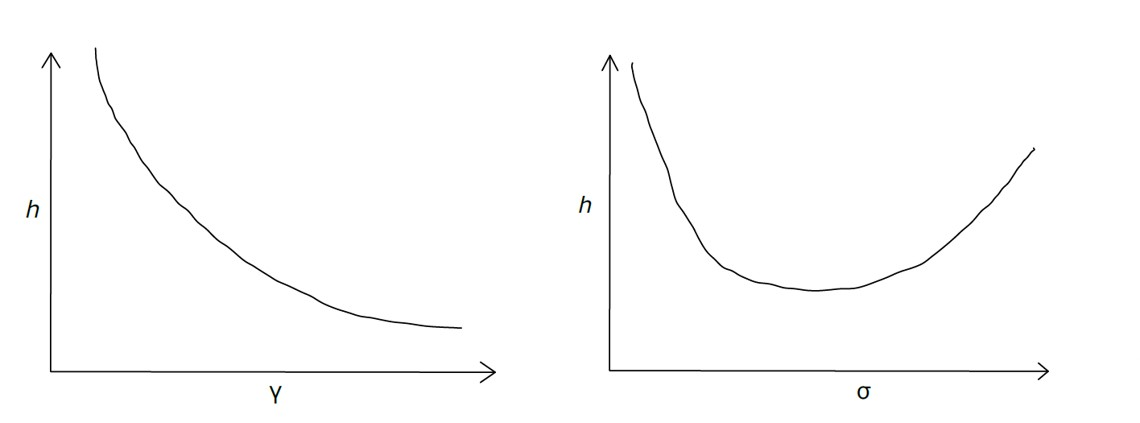
\includegraphics[width=\textwidth]{immagini/Fault.jpg}
\end{figure}

\subsection{Insieme di lavoro}

In una gerarchia di memoria $\mathrm{M}_2\textrm{-}\mathrm{M}_1$, l'insieme di lavoro di un programma (processo) è definito come l'\textit{insieme di pagine} (\textit{blocchi}) che, \textit{se presenti contemporaneamente in $\mathrm{M}_1$, rendono minima la probabilità di fault}.\
L'insieme di lavoro va considerato sia in termini di quante pagine che di quali pagine devono essere possibilmente presenti in $\mathrm{M}_1$ contemporaneamente.

L'obiettivo di una gestione efficiente di una gerarchia di memoria è quello di individuare l'insieme di lavoro e cercare di mantenerlo in $\mathrm{M}_1$.\
A questo scopo, occorre cercare di sfruttare al meglio le proprietà di \textit{località} e, in particolare, di \textit{riuso} di ogni programma.

\section{Gerarchia Memoria Virtuale - Memoria Principale}

\subsection{Spazi di indirizzamento}

Durante la fase di traduzione, il compilatore provvede a scegliere gli indirizzi di memoria per le istruzioni e per i dati di $Q$.\
Viene così definito lo \textit{spazio di indirizzamento logico del processo}, $N$, cioè l'insieme di tutti gli indirizzi, noti a tempo di compilazione e generati dal processore a tempo di esecuzione.

Chiamiamo \textit{spazio di indirizzamento fisico}, $M$, l'insieme degli indirizzi di memoria principale (\textit{indirizzi fisici}) assegnati a un processo quando viene allocato in memoria principale.\
$M$ può coincidere o essere un sottoinsieme dei possibili indirizzi della memoria principale.

\subsection{Allocazione della memoria principale}

Nel caso di allocazione statica della memoria principale, $N$ e $M$ coincidono.\
Per essere eseguito, tutto il processo è interamente caricato da memoria secondaria a memoria principale in un'area nota.

Nel caso di allocazione dinamica della memoria principale, lo spazio $M$ assegnato al processo varia a tempo di esecuzione sia in posizione sia in quantità.\
In generale, non tutto $N$ è allocato contemporaneamente in memoria principale, ma solo una sua parte, possibilmente quella che, istante per istante, permette al processo di reperire la maggior parte delle informazioni (istruzioni e dati) in memoria principale.\
La parte di $N$ allocata in memoria principale varia a tempo di esecuzioni, così come la zona di memoria principale in cui allocare \textit{N}.\
Inoltre, in generale tale zona non è contigua, anche nel caso che $N$ lo sia.

Per un processo $Q$ deve essere definita una funzione di rilocazione, o funzione di traduzione degli indirizzi:
\[\mu_Q: N \rightarrow M\]
La funzione di traduzione degli indirizzi $\mu_Q$, implementata con la Tabella di Rilocazione, viene aggiornata e valutata a tempo di esecuzione per ogni indirizzo logico generato dal processo $Q$ in esecuzione sul processore.\
Ciò avviene con l'ausilio di supporti hardware-firmware particolarmente efficienti:\ l'unità \textit{MMU} che, facente parte della CPU, fa da tramite tra processore e memoria principale, provvedendo a tradurre gli indirizzi da logici a fisici in un solo ciclo di clock; nel caso che $\mu_Q$ non sia definita, \textit{MMU} restituisce l'eccezione al processore.

\subsection{Creazione di processi, caricamento, e commutazione di contesto}

Quando un processo $Q$ esegue una primitiva di \textit{creazione} di un altro processo $R$, questa provoca un \textit{caricamento} di $R$, cioè il trasferimento di informazioni di $R$ da memoria secondaria a memoria principale.\
Una volta creato, $R$ viene posto nello \textit{stato di pronto}.

Il file, che rappresenta il prodotto della traduzione dal programma al processo $R$, contiene diverse informazioni, sotto forma di opportune strutture dati, che verranno utilizzate da funzionalità del supporto durante l'evoluzione del processo stesso:\ in particolare, la struttura dati \textit{descrittori di processo} (\textit{PCB}).

\textit{Il PCB viene inizializzato a tempo di compilazione}, in particolare assegnando i valori costanti con cui inizializzare i registri generali e il contatore istruzioni.

Quando il processo $R$ viene creato, in memoria principale viene compilato anche il suo PCB con il valore che è stato inizializzato a tempo di compilazione.

Quando verrà il turno di $R$ a passare in esecuzione sul processore, ha luogo \textit{la commutazione di contesto}:

\begin{itemize}
    \item l'immagine di RG e di IC viene copiata dall'area facente parte del PCB\textsubscript{R} nei registri RG e nel registro IC.\ In tal modo:
          \begin{itemize}
              \item i registri sono inizializzati come stabilito a tempo di compilazione,
              \item la prima istruzione da eseguire sarà quella all'indirizzo logico di R, stabilito a tempo di compilazione, che è stato scritto in IC;
          \end{itemize}
    \item il processo ($T$) che esce dallo stato di esecuzione provvede a salvare nel proprio $\mathrm{PCB}_T$ i valori correnti di RG e IC.\ In tal modo, quando successivamente \textit{T} tornerà in esecuzione, RG e IC verranno ripristinati con le rispettive immagini presenti nel $\mathrm{PCB}_T$, esattamente secondo lo schema descritto precedentemente, in modo che $T$ possa riprendere l'esecuzione a partire dall'ultima eseguita prima di sospendersi e con i contenuti dei registri generali presenti prima di sospendersi.
\end{itemize}

\subsection{Allocazione dinamica della memoria con paginazione}

Il processo, una volta creato, in ogni istante risulta allocato in uno spazio fisico di memoria principale, che in generale non è né contiguo né completo:\ non tutto il processo risiede contemporaneamente in memoria, e la parte che vi risiede è distribuita in \textit{blocchi}, o \textit{pagine}, di ampiezza fissa e al loro interno contigue, ma sparse in zone diverse della memoria.

In un caso tipico, una pagina è ampia 1K parole con indirizzi logici di 32 bit.\
L'indirizzo logico può dunque essere visto come composto dalla concatenazione di due campi:\ quello dei bit più significativi fornisce l'\textit{identificatore di pagina logica}, IPL, e quello dei bit meno significativi l'\textit{indirizzo all'interno della pagina} o \textit{displacement}.

La funzione di rilocazione del processo $Q$, $\mu_Q$, viene implementata mediante una tabella, detta Tabella di Rilocazione del processo, $\mathrm{TABRIL}_Q$, il cui contenuto è inizializzato a tempo di caricamento/creazione e varia durante l'esecuzione del processo in seguito all'allocazione dinamica di pagine.

\textit{Attraverso la Tabella di Rilocazione la funzione di rilocazione viene applicata alle pagine}.\
L'entrata $i$-esima della Tabella di Rilocazione contiene, tra le altre informazioni:

\begin{itemize}
    \item un \textit{bit di presenza}, \texttt{PRES}, che, se a uno, indica che la pagina logica $i$-esima è presente in memoria principale;
    \item un \textit{identificatore di pagina fisica}, \texttt{IPF}, cioè l'identificatore della pagina di memoria principale dove risiede la pagina logica $i$-esima nel caso che $\mathtt{PRES} = 1$.
\end{itemize}

\begin{figure}[H]
    \centering
    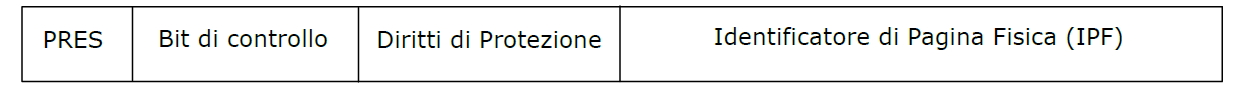
\includegraphics[width=\textwidth]{immagini/Tabril.png}
\end{figure}

\noindent Indichiamo con $x^{\circ} y$ il concatenamento dei valori $x$, $y$ in una stessa unità di informazione.\
Dato l'indirizzo logico $\mathrm{IPL}^{\circ}\mathit{displ}$ generato dal processo $Q$, se $\mathrm{TABRIL}_Q[\mathrm{IPL}].\mathtt{PRES} =1$, allora l'indirizzo fisico corrispondente è dato da $\mathrm{TABRIL}_Q[\mathrm{IPL}].\mathtt{IPF}^{\circ}\mathit{displ}$.

Se $\mathrm{TABRIL}_Q[\mathrm{IPL}].\mathtt{PRES} = 0$, allora viene generata l'eccezione di fault di pagina.

Nello schema di TABRIL è anche indicato il campo ``Bit di controllo'' contenente un bit per ricordare se la pagina è stata modificata e informazioni per implementare la politica di rimpiazzamento.\
Quest'ultima politica, \textit{eseguita dalle funzionalità di gestione della memoria in seguito all'eccezione di fault di pagina}, ha come scopo la scelta della pagina da sostituire; \textit{la scelta che mediamente fornisce il risultato migliore, agli effetti della riduzione della frequenza dei fault di pagina} è la \textbf{LRU} (Least Recently Used).

\subsection{MMU}

La traduzione dell'indirizzo logico e l'eventuale generazione di eccezioni di fault di pagina sono implementate a hardware-firmware nell'unità \textit{MMU} facente parte della CPU.

Al processore P non è visibile come avviene la traduzione degli indirizzi, ma deve comunque essere noto l'\textit{esito} di ogni accesso in memoria.

Per effettuare efficientemente la traduzione dell'indirizzo, \textit{MMU} deve disporre di risorse hardware opportune.\
Occorre allora realizzare in hardware una \textit{tabella accedibile per contenuto}:\ questo componente è chiamato \textbf{Memoria Associativa} (MA) ed è costituita da $C$ registri, ognuno contenente una \textit{chiave}, e altrettanti contenenti i corrispondenti \textit{valori}.

Le uscite dei registri-chiave sono ingressi di $C$ confrontatori, il cui secondo ingresso è costituito dalla \textit{chiave Key} con la quale si vuole effettuare la ricerca.\
Quindi viene effettuato il confronto \textit{simultaneo} di \textit{Key} con tutte le Chiavi in tabella.\
Uno dei confronti è positivo, allora l'indice del registro-chiave relativo fornisce univocamente l'indirizzo della RAM dalla quale leggere il Valore corrispondente a \textit{Key}; in caso di tutti i confronti negativi, l'evento negativo viene segnalato attraverso il valore di un bit di Fault.

Una parte di Tabella di Rilocazione TABRIL è mantenuta, dinamicamente, nella Memoria Associativa MA nella PO della \textit{MMU}.\
\textit{Le chiavi sono gli identificatori di pagina logica IPL}, mentre \textit{i valori sono i corrispondenti contenuti TABRIL[IPL] della Tabella di Rilocazione}.

Normalmente, si mantengono in MA le entrate di TABRIL \textit{usate più di recente}:\ questo permette di rendere trascurabile la probabilità che l'entrata di interesse non risieda in MA.\
In caso che venga generato un fault di MA, \textit{MMU} provvede a copiare in MA l'entrata di TABRIL corrispondente alla pagina logica riferita, sostituendo l'entrata usata meno di recente, per questa ragione all'atto della commutazione di contesto, quando viene posto in esecuzione il processo $Q$, \textit{l'indirizzo di} $\mathrm{TABRIL}_Q$ deve essere comunicato a \textit{MMU}, che lo mantiene in un suo registro interno.

\section{Architettura con cache}

\subsection{Struttura della CPU con cache}

\begin{figure}[H]
    \centering
    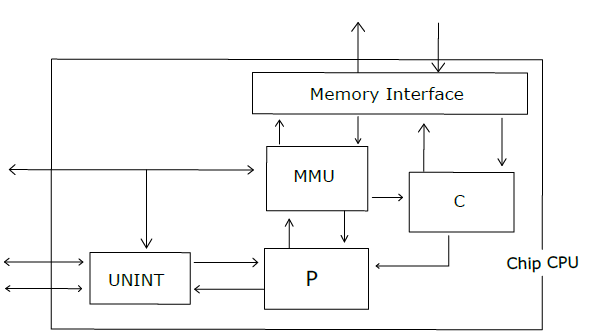
\includegraphics[width=0.7\textwidth]{immagini/CPU_cache.png}
\end{figure}

\noindent Nel caso di successo nella rilocazione dell'indirizzo logico (di memoria virtuale), \textit{MMU} passa la richiesta con l'indirizzo fisico (di memoria principale) all'unità cache $C$.\
Questa provvede \textit{all'ulteriore traduzione da indirizzo di memoria principale a indirizzo di memoria cache}, nel caso che la funzione di traduzione sia definita; in caso di insuccesso (cache \textit{fault}) ha luogo il \textit{trasferimento} del blocco di memoria principale richiesto in uno dei blocchi di $C$, in generale sostituendone uno già presente scelto mediante un opportuno algoritmo di rimpiazzamento.\
Il trasferimento del blocco è, a differenza del fault di memoria virtuale, del tutto \textit{invisibile} a P.

Occorre prevedere un metodo per il trattamento delle \textbf{scritture nella memoria cache}:

\begin{enumerate}
    \item nel metodo\textit{ Write Back}, il blocco modificato viene ricopiato nel livello superiore di memoria solo all'atto della sostituzione del blocco stesso nel livello superiore o alla terminazione del processo;
    \item nel metodo \textit{Write Through}, ogni modifica della cache è effettuata immediatamente e contemporaneamente anche in memoria principale.
\end{enumerate}

\subsection{Metodi di indirizzamento della cache}

I principali metodi sono chiamati \textbf{diretto}, \textbf{completamente associativo} e \textbf{associativo su insiemi}.

\subsubsection{Metodo diretto}

In questo caso ogni blocco di memoria principale può essere trasferito solo in un bene determinato blocco della cache:\ esiste dunque uno o un solo blocco della cache in cui una certa informazione può risiedere.

Si può scegliere di adottare una semplice funzione di corrispondenza tra blocchi, tipicamente la funzione \textit{modulo}, secondo la quale l'identificatore \textit{BC} del blocco di cache è dato da:\ \textit{BC = BM mod NC}, dove \textit{BM} indica l'identificatore del blocco di $M$ e \textit{NC} il numero di blocchi in cache.

Se, come di regola, \textit{NC} è una potenza di 2, il campo \textit{BM} dell'indirizzo di $M$ contiene l'informazione \textit{BC} direttamente nei $\log_2NC$ bit meno significativi, mentre i restanti bit di \textit{BM}, indicati con \textit{TAG}, \textit{TAG = BM div NC} identificano il blocco di \textit{M} all'interno dell'insieme di tutti quelli che corrispondono a quel particolare blocco di $C$ identificato da \textit{BC}.

In questo metodo dunque la funzione di traduzione è immediata, essendo l'eventuale \textit{BC} corrispondente a \textit{BM} già presente nello stesso indirizzo fisico.\
L'accesso alla cache è dunque effettuato direttamente.\
Il sistema dovrà mantenere una \textit{Tabella di Corrispondenza}, avente \textit{NC} posizioni:\ ogni posizione contiene il valore del \textit{TAG} corrispondente al blocco di $M$ effettivamente presente nel blocco di cache individuato da \textit{BC}.

Con il metodo diretto tenendo conto anche della presenza della \textit{MMU}, il tempo di accesso alla memoria cache, in assenza di fault è $t_c = 2\tau$ che rappresenta il minimo valore possibile con il protocollo a domanda e risposta.

I vantaggi di questo metodo sono la velocità e la semplicità.\
Per contro esso presenta uno svantaggio:\ quando occorre accedere ripetutamente a coppie di informazioni che stanno in blocchi di $M$ corrispondenti allo stesso blocco di $C$, il numero di fault risulta molto elevato.

Rispetto ai valori per la probabilità di fault $h$ calcolati per gli altri metodi si può verificare una degradazione fino al 50\%, a parità di ampiezza dei blocchi e capacità dalla cache.

Un caso in cui l'inconveniente descritto è poco rilevante è quello delle istruzioni.\
Suddividendo, come di regola, la cache in una \textbf{cache istruzioni} o una \textbf{cache dati}, in diversi sistemi la prima adotta il metodo diretto.

\subsubsection{Metodo completamente associativo}

Questo metodo, a differenza del precedente, offre la massima flessibilità circa la corrispondenza tra blocchi di $M$ e blocchi di $C$:\ ogni blocco di $M$ può risiedere in \textit{qualsiasi} blocco di $C$.

La parte \textit{BM} dell'indirizzo fisico generato è usata come chiave per una ricerca tabellare mediante la quale implementare la funzione di traduzione dell'indirizzo.\
Per ragioni di efficienza, tale \textit{Tabella di Corrispondenza} non può che essere realizzata con una memoria associativa:\ la sua uscita fornisce, se non si verifica fault, l'identificatore del blocco di $C$.

Tenendo conto anche della presenza della \textit{MMU}, il tempo di accesso alla memoria cache, in assenza di fault, è:\ $t_c = 3\tau$.

Assumendo che in ciclo di clock sia possibile stabilizzazione di un solo componente logico di memoria.

Questo metodo fornisce la massima flessibilità al prezzo di un maggiore tempo di accesso e di un aumento di costo dovuto alla memoria associativa.

\subsubsection{Metodo associativo su insiemi}

Questo metodo approssima soddisfacentemente sia la flessibilità del metodo completamente associativo che la semplicità del metodo diretto.

Ogni blocco di memoria principale è fatto corrispondere a un ben determinato \textit{insieme} di blocchi della cache, potendo essere però allocato in uno qualsiasi dei blocchi di tale insieme.

Similmente a quanto fatto nel Metodo Diretto, adottiamo la funzione \textit{modulo} per esprimere la corrispondenza tra blocchi di $M$ e insiemi di cache; l'identificatore \textit{SET} dell'insieme dei blocchi di cache è dato da:\ \textit{SET = BM mod NS} dove \textit{BM} indica l'identificatore del blocco $M$ e \textit{NS} il numero di insiemi di blocchi della memoria di cache.\
Se, come di regola NS è una potenza di 2, il campo \textit{BM} dell'indirizzo di $M$ contiene l'informazione \textit{SET} \textit{direttamente} nei $\log_2NS$ bit meno significativi, mentre i restanti bit di \textit{MB}, indicati con \textit{TAG}, \textit{TAG = BM div NS} identificano il blocco di $M$ all'interno dell'insieme di tutti quelli che corrispondono a quel particolare insieme di blocchi di $C$ identificato da \textit{SET}.

Tenendo conto anche della presenza della \textit{MMU}, il tempo di accesso alla memoria cache, in assenza di fault, è $t_c = 2\tau$.

È stato verificato mediante simulazioni ed esperimenti che insiemi di 8 blocchi permettono di ottenere una \textit{probabilità di fault} molto vicina a quella del metodo completamente associativo.\
D'altra parte, la logica necessaria è paragonabile a quella del metodo diretto.

\subsection{Modello dei costi}

Si vuole valutare il tempo di completamento del programma e il tempo di servizio per istruzione.\
L'\textit{efficienza relativa} dell'architettura con cache, $\epsilon$, è valutata come il rapporto tra tempo di completamento $T_{c-0}$ \textit{in assenza di fault di cache} e il tempo di completamento \textit{effettivo} $T_c$ considerando la penalità dovuta ai fault $T_{\mathit{fault}}$.

Il tempo di completamento è valutato come:\ \[T_c = T_{c-0} + T_{\mathtt{fault}}\]
$T_{\mathit{fault}}$ si valuta come:\ \[T_{\mathit{fault}} = N_{\mathit{fault}} + T_{\mathit{transf}}\]
Dove

\begin{itemize}
    \item \textit{N\textsubscript{fault}} è il numero medio di fault di cache che hanno luogo durante tutta l'esecuzione dello specifico programma,
    \item \textit{T\textsubscript{transf}} è il tempo necessario per effettuare il trasferimento di un blocco di cache dal livello superiore alla cache primaria.
\end{itemize}

\noindent Da $T_c$ si ricavano il tempo di servizio $T$:\ \[T=\frac{T_c}{N_{\mathit{istr}}}\]\\
Dove $N_{\mathit{istr}}$ è il numero medio di istruzioni eseguite per completare il programma, e l'efficienza relativa:\ \[\epsilon = \frac{T_{c-0}}{T_c}\]

\subsubsection{Trasferimento di blocchi dalla memoria principale}

Nel caso di trasferimento del blocco da $M$ a $C$, poiché dobbiamo leggere $\sigma$ parole a indirizzi consecutivi, una soluzione adatta è dunque l'organizzazione di memoria modulare interallacciata ottenendo così:

\[T_{\mathit{transf}} = 2T_{tr} + \frac{\sigma}{m}\tau_M+m\tau\]

\subsection{Cache a più livelli}

La soluzione della memoria interallacciata riesce solo in parte a soddisfare il requisito di minimizzare la
latenza del trasferimento dei blocchi.\
Occorre considerare che sono ancora significative le latenze dei singoli moduli di memoria e dei collegamenti.\
Si deve perciò ricorrere a \textit{tecnologie di memoria che riducano la latenza di per sé}, senza necessariamente introdurre il parallelismo.\
In pratica, questo principio conduce all'introduzione di ulteriori livelli di cache, in particolare la \textbf{cache secondaria} integrata sullo stesso chip CPU con la stessa tecnologia della primaria.

La capacità di $C_2$ è un ordine di grandezza superiore a $C_1$, con blocchi più ampi.\
$C_1$ è utilizzata da un solo processo alla volta.\
In $C_2$, invece, sono normalmente presenti blocchi appartenenti a più processi in stato di pronto.

Il principio è estendibile alla \textbf{cache terziaria}, anch'essa on-chip quando prevista.

Combinando le due soluzioni discusse (\textit{$M$ esterna interallacciata per avere parallelismo), $C_2$ ed eventualmente $C_3$ on-chip per abbattere le latenze}, si giunge alla soluzione architetturale più frequente, nella quale la cache primaria funziona on demand, ma i livelli superiori di cache funzionano con prefetching, e le memorie esterne al chip CPU hanno organizzazione interallacciata.\
Vale la pena notare che a parità di capacità complessiva $\gamma$, mantenere la distinzione tra cache primaria e  secondaria on-chip è conveniente rispetto ad avere soltanto un'unica cache primaria di capacità $\gamma$.\
Infatti:

\begin{itemize}
    \item la cache primaria contiene solo informazioni del processo in esecuzione, mentre la cache secondaria può mantenere informazioni di più processi, e quindi essere pronta a trasferire blocchi in/da cache primaria in caso di commutazione di contesto;
    \item blocchi della cache secondaria hanno dimensione adatta al trasferimento con la memoria principale (o cache terziaria);
    \item la cache secondaria può trasferire blocchi dalla memoria principale (o cache terziaria) in parallelo all'esecuzione del processo e all'uso della cache primaria, ad esempio anticipando blocchi del processo in esecuzione o di altri processi con la tecnica del \textit{prefetching}.
\end{itemize}

\noindent Queste caratteristiche fanno sì che, in molti programmi, si possa assumere \textit{trascurabile la probabilità di fault in $C_2$} in seguito ad una richiesta di $C_1$.


\chapter{Ingresso - Uscita}

\section{Compiti delle unità di I/O e cooperazione con i processi della CPU}

Ogni unità di I/O svolge il compito di interfacciare, nei confronti dell'unità centrale, un certo tipo di dispositivo periferico, come dischi fissi e altre memorie di massa, stampanti, scanner, dispositivi audio, dispositivi video, interfacce di rete\ \dots

\subsection{Unità di I/O e driver}

Oltre che compiti d'interfacciamento, una unità di I/O svolge, in generale, anche compiti di \textit{pre-elaborazione}, o \textit{post-elaborazione}, nei confronti delle funzionalità di trasferimento dati tra unità centrale e dispositivi periferici e in molti casi svolge anche compiti più sofisticati di \textit{gestione} e \textit{controllo del dispositivo}.

In effetti, il confine tra funzionalità delegate al processore e funzionalità delegate all'unità di I/O per la gestione di un dispositivo è molto sfumato.\
Normalmente, a livello di sistema sono previsti degli appositi programmi, o processi, detti \textit{driver} dei dispositivi periferici, aventi appunto il compito di eseguire alcune delle funzionalità necessarie per gestire al meglio tali dispositivi nei confronti dei processi utente.\
Una parte di tali funzionalità, quelle più critiche in termini di prestazioni, viene realizzata ``a firmware'' nelle unità di  I/O, mentre quello meno critiche vengono realizzate ``a software'' nei driver.

\subsection{Cooperazione processi - unità di I/O}

Le elaborazioni svolte dalle unità di I/O possono essere considerate dei veri e propri processi, detti \textbf{processi esterni}, eseguibili solo sui ``processori'' costituiti dalle unità di stesse.\
Tali funzionalità possono essere, di fatto, implementate:

\begin{itemize}
    \item a livello firmware, in unità specializzate,
    \item a livello assembler, ``embedded'' in processori general-purpose con propria memoria e MMU.
\end{itemize}

\noindent In ogni caso, occorre implementare anche le primitive per la cooperazione con i processi eseguibili dalla CPU (\textit{processi interni}).\
Nel caso più semplice, un'unità di I/O comunica solo con il proprio processo Driver, ma questa non è assolutamente una regola.\
In particolare, occorre che il processore sia avvertito, \textit{in modo asincrono rispetto all'esecuzione del processo interno corrente}, di eventi comunicati da un'unità di I/O.\
Il meccanismo delle interruzioni serve proprio a questo scopo.

\subsection{Interruzioni ed eccezioni}

La distinzione fondamentale tra questi due tipi di eventi è la seguente:

\begin{itemize}
    \item le \textit{eccezioni} sono eventi \textit{sincroni} rispetto all'esecuzione del processo corrente:\ infatti, esse si verificano in quanto provocati dalla stessa computazione in corso sul processore, la quale è espressa in modo da testare esplicitamente la presenza di ben determinate eccezioni a istanti ben determinati;
    \item le \textit{interruzioni} sono eventi \textit{asincroni} rispetto all'esecuzione del processo corrente:\ infatti, essi non sono provocati dalla computazione in corso sul processore, bensì da computazioni che evolvono parallelamente a essa su unità di I/O (o altri processori); non avrebbe senso che il processo eseguito dal processore testasse la presenza di ben determinate interruzioni a istanti scelti arbitrariamente; convenzionalmente si sceglie allora la fine del microprogramma di ogni istruzioni per testare la presenza di una qualsiasi interruzione, proseguendo subito alla chiamata dell'istruzione successiva se non sono attualmente segnale interruzioni presenti.
\end{itemize}

\subsection{Trasferimento dati}

Distinguiamo due aspetti riguardanti l'architettura di tale sottosistema:
\begin{enumerate}
    \item il \textit{trasferimento di dati} tra Unità Centrale (CPU, M) e unità di I/O,
    \item comunicazioni di \textit{eventi asincroni} da unità di I/O a Processore mediante il meccanismo delle  interruzioni.
\end{enumerate}

\noindent Il trasferimento dati tra Unità Centrale e unità di I/O avviene quando un processo, PROC, in esecuzione sulla CPU vuole inviare dati a, o ricevere dati da, un'unità di I/O.\
PROC può essere il Driver dell'unità di I/O oppure un qualsiasi altro processo.

I dati trasferiti possono essere di tipo elementare, implementati come parole o byte, o, più frequentemente, \textit{blocchi} di dati.

Distinguiamo due modelli:
\begin{itemize}
    \item \textbf{Direct Memory Acces}s (\textit{DMA}):\ il trasferimento di dati tra I/O e memoria principale, e viceversa, avviene indipendentemente attraverso un canale distinto, utilizzando uno o più \textit{Bus DMA}.\ Questi trasferimenti, per definizione, avvengono \textit{in parallelo all'elaborazione in corso sul processore}.
    \item \textbf{Memory mapped I/O} (\textit{MMI/O}):\ poiché a ogni unità di I/O è associata a una certa capacità di memoria locale, questa è \textit{indirizzabile direttamente anche dal processore P}; il trasferimento dati tra P e I/O avviene dunque attraverso letture e scritture da parte di P nelle memorie locali di I/O.\ In altre parole, un programma in esecuzione su P \textit{vede le unità di I/O come memoria}.\ Anche in questo caso gli accessi alla memoria locale di I/O da parte di una delle due unità - P o I/O - \textit{avvengono in parallelo} all'elaborazione dell'altra unità.
\end{itemize}

\noindent Nel modello DMA, M è condivisa tra P e le unità di I/O operanti in DMA.

Nel modello MMI/O, ogni memoria locale di unità di I/O è condivisa tra P e tale unità.

\section{Trattamento delle interruzioni}

Come detto più volte, a livello firmware le interruzioni hanno il significato di segnali di richiesta all'arbitro del Bus di I/O di inviare un messaggio di I/O su tale bus.\
Ai livelli superiori, il significato di un'interruzione è di segnalare, attraverso il messaggio di I/O, un \textbf{evento}.\
Una procedura del processo in esecuzione, che chiameremo \textbf{Handler} dell'interruzione, provvede a compere le azioni necessarie per trattare l'evento stesso.

A ogni evento che le unità di I/O possono comunicare corrisponde un proprio Handler.

Il trattamento dell'interruzione deve prevede due fasi:

\begin{itemize}
    \item una prima \textbf{fase firmware}, nella quale il processore accetta l'interruzione, attende il messaggio di I/O e usando tale messaggio come parametro, \textit{chiama} una procedura indicata con \textit{Routine di interfacciamento Interruzioni}.\ Il messaggio di I/O conterrà l'identificatore dell'evento e un dato elementare;
    \item una seconda \textbf{fase assembler}, nella quale viene eseguita la Routine di Interfacciamento Interruzioni e la procedura Handler dell'evento comunicato con l'interruzione.
\end{itemize}

\noindent La Routine di Interfacciamento Interruzioni serve a permettere alla fase firmware di collegare \textit{qualunque} istruzione di \textit{qualunque} processo agli Handler, \textit{svincolando la progettazione firmware del processore della conoscenza a priori degli Handler stessi}.

\begin{figure}[H]
    \centering
    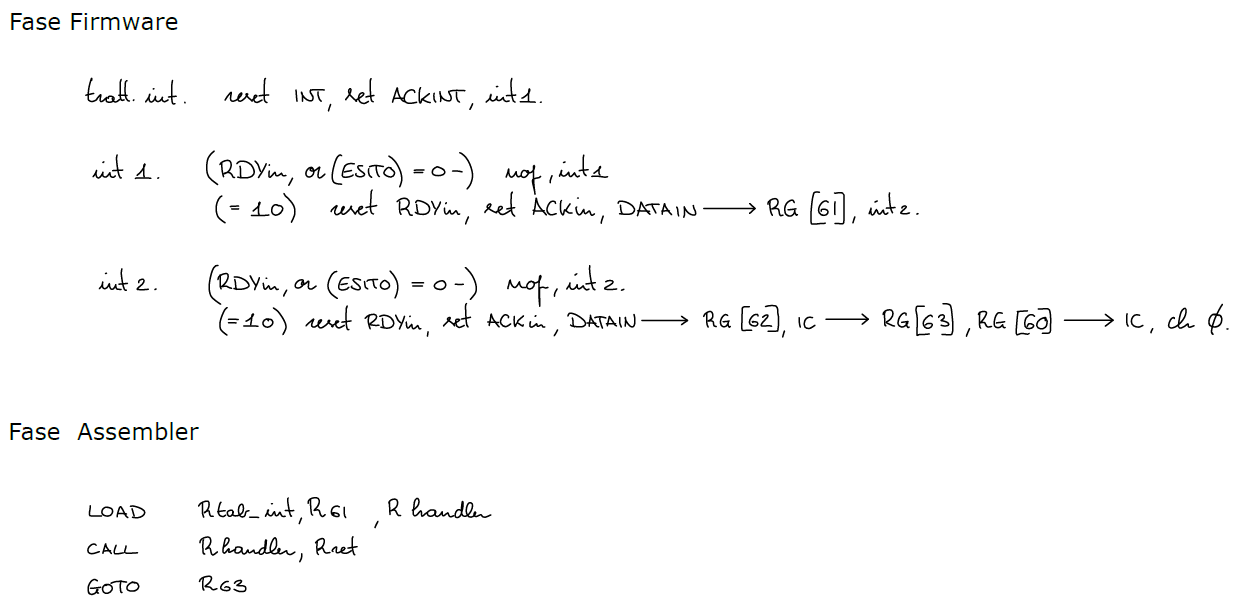
\includegraphics[width=\textwidth]{immagini/Handler.png}
\end{figure}
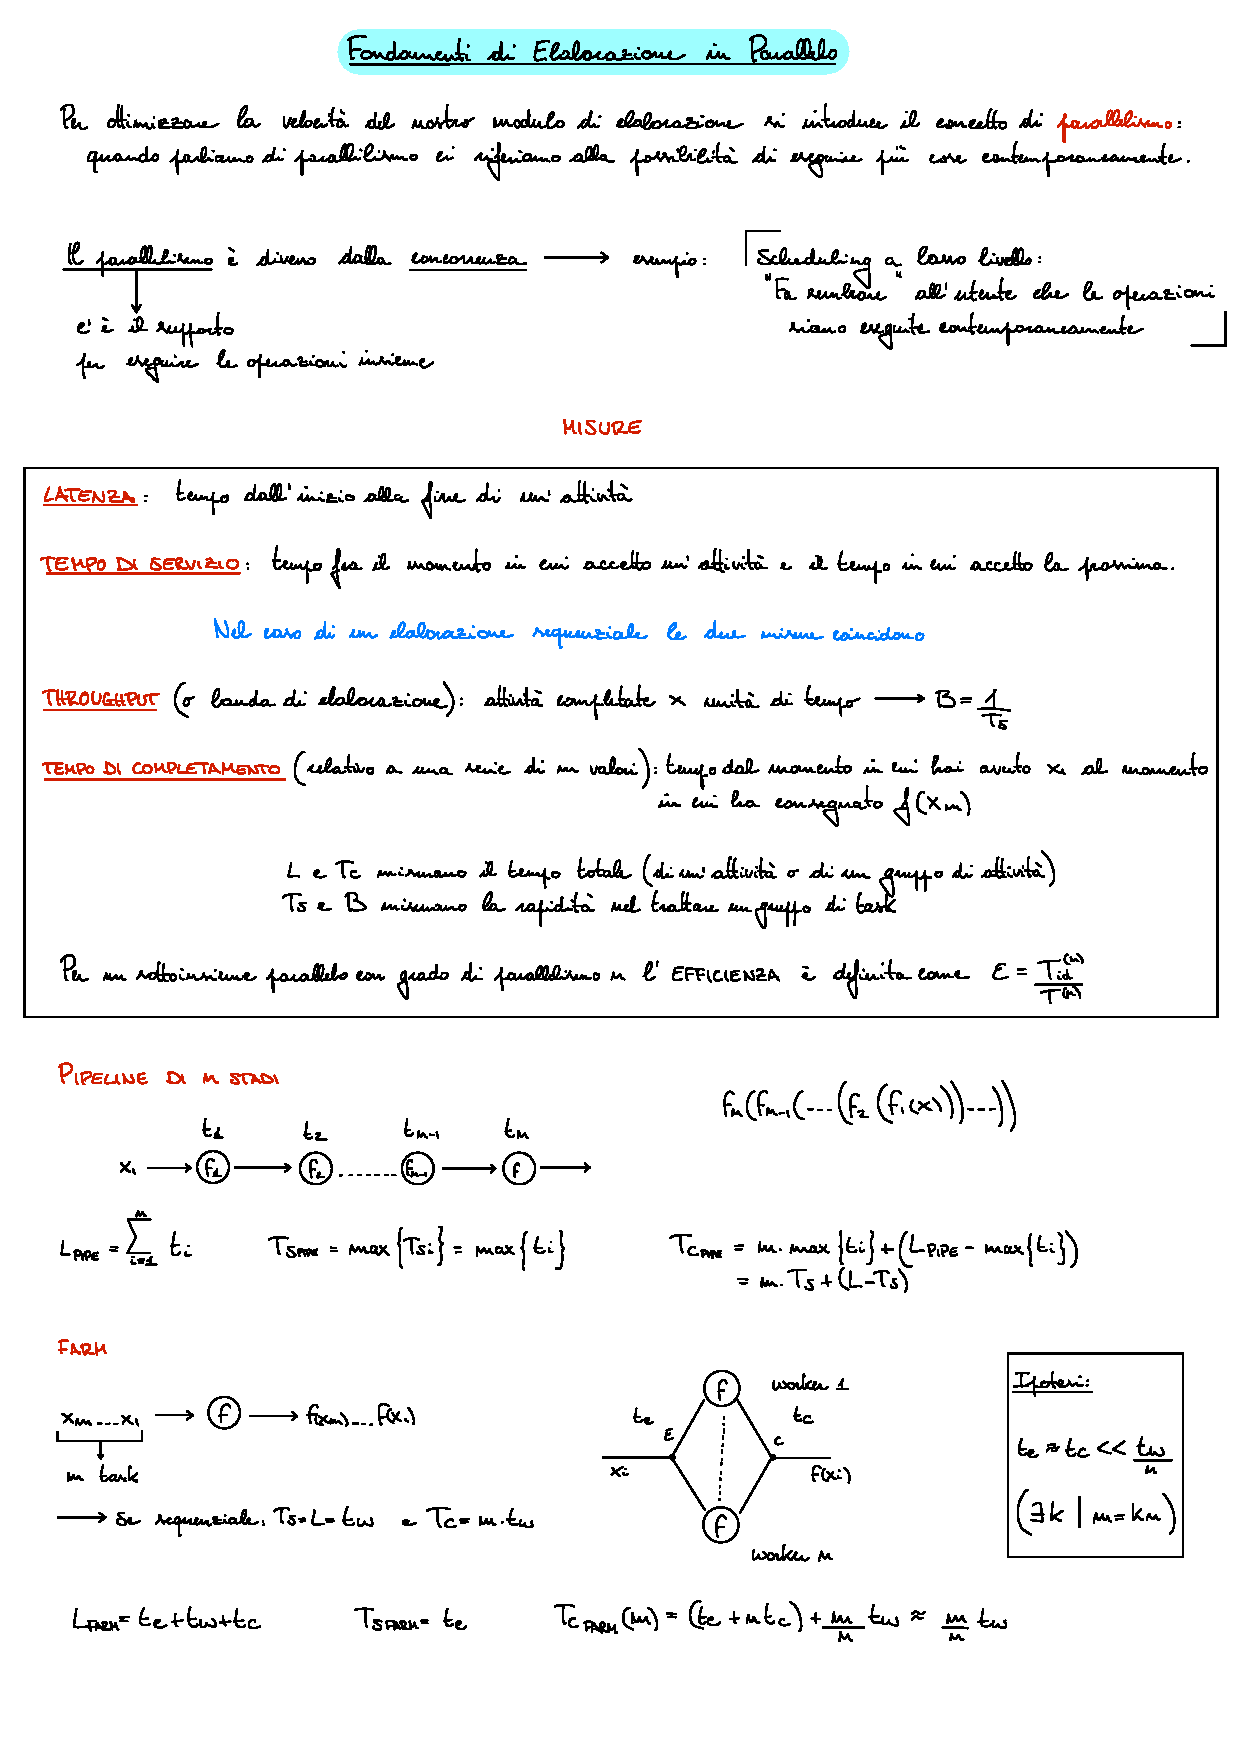
\includepdf[pages=-]{Elaborazione_parallelo}




\end{document}
